\chapter{ALNDOTPLOT: VISUAL REPRESENTATION AND ANALYSIS OF PAIRWISE ALIGNMENTS}  \label{ch:alndotplot}

\section{Introduction}
% Nature of the problem
% * sequence alignment is hard
% * There's been improvement because it's an important problem
% * yet comparison between sequence alignments has not seen any major developments - describe current tools
The analysis of biological sequences is the inference of unique and unobservable evolutionary events at the DNA level \citep{morrison_MSA_2018}. Alignment inference is an essential step required to address questions across multiple branches of biology, including molecular biology, microbiology, and ecology. The field has seen substantial progress since modern sequence alignment began with the computer-adaptable algorithm of Needleman and Wunsch \citeyearpar{Needleman1970}, replacing the arduous manual arrangement of residues as the default method for sequence alignment.

% Current knowledge and limitations
% * tools and methods to evaluate sequence alignment are almost as important as the alignment algorithms themselves
% * current options to evaluate the accuracy of alignments are these, with these limitations
% * probably a couple of paragraphs grouping tools by type

The development of sequence alignment methods has experienced a continuous effort to improve both their accuracy and speed. The quality of sequence alignments directly impacts the reliability of downstream analyses, and thus, alignment evaluation plays a pivotal role in quality control. Existing evaluation methods can be divided into metrics and scores that summarize similarities between alignments and tools that quantify the uncertainty associated with each column of an alignment. A limitation of these methods is that they can compare a summary metric between two alignments or provide site information about an alignment, but cannot combine both approaches. While aligners typically report a single best result using an evolutionary or scoring model, equally optimal (equivalent) alignments often exist and are rarely reported. However, equivalent alignments and suboptimal alternatives are common in sampling and multiple sequence refinement. Being able to perform a thorough comparison between such alignments can be very valuable for understanding how the underlying biological models work. This can also lead to more detailed comparisons of different methods in validating sequence aligners, improve the algorithms that search for suboptimal alignments in multiple sequence refinement, and better assess sampling results.

\subsection{Alignment Accuracy}

% explain B - metrics that summarize alignment similarities - SOP, TC, d_{seq}
Popular alignment similarity scores include sum-of-pairs (SP) and total column score (TC). SP is the percentage of correctly aligned residue pairs in an alignment, which measures how well pairs of sequences are aligned, while TC is the percentage of correctly aligned columns in an alignment, testing the ability to align all sequences correctly \citep{thompson2005balibase}. In the case of pairwise alignment, both metrics are identical. A more informative set of metrics that consider indels and the evolutionary history of events in a phylogenetic tree was put forth by Blackburne and Whelan \citeyearpar{metrics_blackburne_whelan_2011}. These metrics range from zero to one and can be interpreted as the probability that a randomly selected residue will be aligned to a different location against a sequence that does not contain such residue. Notably, similarity and distance metrics are easily scalable to compare results over large datasets. However, they struggle to find specific portions where alignments diverge and what are their differences.

% explain A - tools that quantify position uncertainty - GUIDANCE, T-COFFEE, MUMSA
Tools and methods that quantify alignment uncertainty include Heat or Tails \citep{landan2007heads}, a method that considers the probability distribution of possible placements for each sequence within a multiple sequence alignment; GUIDANCE \citep{penn2010guidance}, which uses bootstrap algorithms; GUIDANCE 2 \citep{sela2015guidance2}, which combines three sources of uncertainty: co-optimal solutions, guide tree instability, and opening gap penalty; ZORRO \citep{wu2012zorro}, based on hidden Markov models; and MUMSA \citep{lassmann2005mumsa}, which calculates the portion of identically aligned regions; and posterior decoding, a popular method used in the context of Markov models that calculates the probability of each state in the alignment path and is particularly useful when many different paths have almost the same probability as the most likely one. These methods provide information about the reliability of each column in an alignment and identify uncertain sections, allowing researchers to remove them to prevent errors that may bias downstream analysis. While these metrics can help improve the quality of genomic pipeline results, they are also limited to analyzing one alignment at a time.

\subsection{Alignment Visualization}

A common feature shared among the alignment uncertainty applications described above is their display of confidence scores and the alignment in matrix form (Fig.~\ref{fig:msa-example}). This format of alignment visualization provides a representation of an alignment, where residues are typically colored by type and are supported by numerous software packages and web-based tools (e.g., \citealp{zhou2022ggmsa}; \citealp{yachdav2016msaviewer}). A matrix representation of an alignment displays two or more aligned sequences as rows, with each column representing a site. However, while this format is intuitive, it does not allow comparing two or more alignments.

\begin{figure}[!ht]
    \centering
    % \resizebox{0.9\textwidth}{!}{
    \definecolor{colorY}{RGB}{255,255,51}   % YELLOW
\definecolor{colorG}{RGB}{77,175,74}    % GREEN
\definecolor{colorB}{RGB}{55,126,184}   % BLUE
\definecolor{colorR}{RGB}{228,26,28}    % RED
\definecolor{colorGy}{RGB}{153,153,153} % GRAY
\definecolor{colorP}{RGB}{152,78,163}   % PURPLE

\begin{tikzpicture}[node distance=1mm,font=\footnotesize]
\tikzstyle{aln}=[matrix of nodes, nodes in empty cells,fill=colorGy!20]
\newcommand{\A}{\textcolor{colorP}{\textbf{A}}}
\newcommand{\C}{\textcolor{colorG}{\textbf{C}}}
\newcommand{\G}{\textcolor{colorB}{\textbf{G}}}
\newcommand{\T}{\textcolor{colorY}{\textbf{T}}}

\matrix (msa)[aln] {
\C\A\T & \A\A\G & \C\G\G & \T\C\G & \G\A\C & \verb|---|\\
\C\A\G & \C\A\G & \C\G\G & \T\C\G & \G\A\C & \A\C\G\\
\C\A\T & \C\A\G & \C\G\G & \T\C\verb|-| & \verb|--|\C & \A\C\A\\
\C\A\T & \C\A\G & \C\C\G & \T\C\G & \G\A\C & \A\C\G\\
};
\end{tikzpicture}
    \caption[Multiple Sequence Alignment Plot]{Example of a DNA multiple sequence alignment visualization in matrix form. Every row corresponds to a sequence and every column is a position in the alignment. Nucleotides are colored by type and gaps are shown in black.}
    \label{fig:msa-example}
\end{figure}

% An additional and perhaps less used visualization method is dot plots.
% Describe dot plots, including what they are and represent, their use cases, and their limitations.
Dot plots are an additional visual representation tool used to compare two sequences that facilitate the identification of similarities, differences, and underlying patterns, introduced by Gibbs and McIntyre \citeyearpar{gibbs1970dotplot}. They consist of a matrix where one sequence is displayed on the x-axis, left to right, and the other on the y-axis, top to bottom, and using dots indicate matching residues between the sequences. Conversely, mismatching nucleotides are left blank. Note that gap symbols are typically not considered in dot plots as they evaluate unaligned sequences.

In biological sequence analysis, dot plots are suitable for identifying regions of similarity between sequences, evidenced by diagonal lines of dots that run left to right and top to bottom. The length and pattern of these contiguous dots provide insight into the nature and extent of the similarity. In addition, dot plots are used to identify specific biological events, including repeated regions, tandem repeats, palindromic regions, and microsatellite patterns (Fig. \ref{fig:dotplot-patterns}). This illustrates that dot plots are a simple and versatile tool for comparing pairs of unaligned sequences.

\begin{figure}[!ht]
    \centering
    \scalebox{1}{\begin{tikzpicture}
    % First square
    \draw (0,0) rectangle (4,4);
    \draw (0,4) -- (4,0);
    \node (a) at (0.3,0.3) {a)};

    % Second square
    \draw (5,0) rectangle (9,4);
    \draw (5,4) -- (9,0);
    \draw (7,3) -- (8,2);
    \draw (6,2) -- (7,1);
    \node (b) at (5.3, 0.3) {b)};

    % Third square
    \draw (0,-1) rectangle (4,-5);
    \draw[dashed] (0,-1) -- (4,-5);
    \node (c) at (0.3, -4.7) {c)};

    % Fourth square
    \draw (5,-1) rectangle (9,-5);
    \draw (5,-1) -- (6.5,-2.5);
    \draw (6.5,-3.5) -- (8,-5);
    \node (d) at (5.3, -4.7) {d)};

    % Sequences
    \draw[->] (-0.5,3) -- (-0.5,-4);
    \draw[->] (1,4.5) -- (8,4.5);
    \node (T1) at (4.5,5) {Sequence T$_1$};
    \node[rotate=90] (T3) at (-1,-0.5) {Sequence T$_2$};
\end{tikzpicture}}
    % 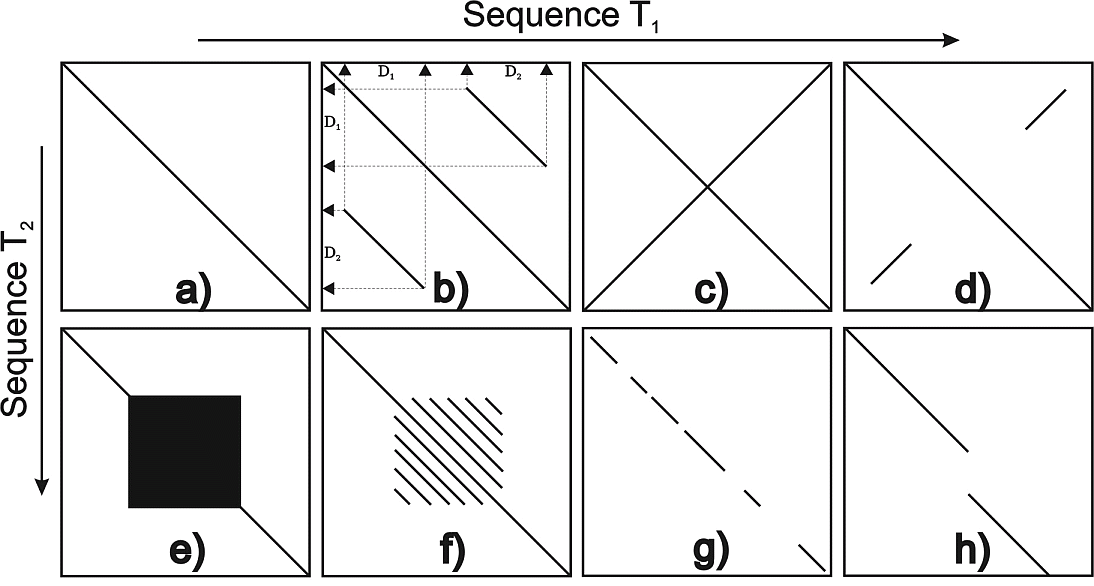
\includegraphics[width = \textwidth]{chapter4/figures/dotplot-patterns.png}
    \caption[Overview of patterns found in dot plots]{. Overview of characteristic patterns in dot plots.
    \textbf{a)} A continuous main diagonal shows perfect similarity.
    \textbf{b)} Parallels to the main diagonal indicate repeated regions on different parts of the sequences.
    \textbf{c)} When the diagonal is a discontinuous line this indicates that the sequences T$_1$ and T$_2$ share a common ancestor.
    \textbf{d)} Partial deletion in sequence T1 or insertion in sequence T2. Work modified from \citealp{schulz2008code10}}
    \label{fig:dotplot-patterns}
\end{figure}

\subsection{Comparison of Pairwise Alignments}
% Then aims and study relevance - I developed AlnDotPlot to address (some of) these limitations.
% General description and impact.
% Sampling, compare alternative and suboptimal alignments, algo más?

The tools described above provide valuable and scalable algorithms for measuring distance or scoring similarity between alignments and methods for identifying uncertain regions within alignments. However, they cannot provide detailed information about how and where alignments differ. To fill this gap, I have developed AlnDotPlot, a visual tool inspired by traditional dot plots that can compare alternative pairwise alignments and is available as an R package. AlnDotPlot can provide a detailed comparison between a handful of pairwise alignments, identify patterns in hundreds of alignment sampling results, and find short base pair differences among alignments of a few kilobases. This software combines the simple nature of dot plots with features to analyze pairwise sequence alignments.

\section{Implementation}

AlnDotPlot can generate alignment dot plots that compare sets of pairwise alignments. This R package can read in alignments in FASTA format and produce results in PDF and TEX format. Internally, the alignment information is converted into matrices, which are in turn, used to create the dot plots. I use the \textit{tikzDevice} R package to create the final results for its versatility and accuracy \citep{sharpsteen2023tikzdevice}. The following sections describe the different models and their implementation and use cases. AlnDotPlot is available as an R software package at \url{https://www.github.com/jgarciamesa/alndotplot}.

\subsection{From Alignment to Dot Matrix}
% Explain how to go from alignment to dot plot

AlnDotPlot generates different alignment dot plots given a set of pairwise alignments. To generate these figures, the first step is to read in the pairwise alignments. Next, the alignment information must be transformed into a dot matrix, which stores this information in a conventional two-dimensional matrix. Based on the different model designs, I have implemented two types of dot matrices. For the simplest model, a traditional dot plot, the dot matrix records only the positions within the alignments involving substitutions (matches and mismatches).
Given two sequences $s$ and $v$, this dot matrix has dimensions $|s|$ by $|v|$, where each row corresponds to symbols in $s$ and every column to symbols in $v$. Every cell in the matrix represents a symbol from $s$ that matches (or mismatches) with a symbol in $v$. The value in every cell is the count of substitutions between these symbols across all input alignments. Figure \ref{fig:aln2matrix-traditional} showcases a sample alignment and its corresponding traditional dot matrix.

\begin{figure}[!ht]
    \centering
    % \begin{multicols}{3}
    \begin{subfigure}[c]{0.4\textwidth}
        \centering
        \vspace*{-7em}\begin{tikzpicture}[node distance=5mm,font=\footnotesize]
\tikzstyle{aln}=[matrix of nodes, nodes in empty cells]

\definecolor{colorY}{RGB}{255,255,51}   % YELLOW
\definecolor{colorG}{RGB}{77,175,74}    % GREEN
\definecolor{colorB}{RGB}{55,126,184}   % BLUE
\definecolor{colorR}{RGB}{228,26,28}    % RED
\definecolor{colorGy}{RGB}{153,153,153} % GRAY

\newcommand{\B}[1]{\textcolor{colorB}{\textbf{#1}}}
\newcommand{\R}[1]{\textcolor{colorR}{\textbf{#1}}}
\newcommand{\G}[1]{\textcolor{colorG}{\textbf{#1}}}

\matrix (aln1)[aln] {
 % \textbf{Aln 1} & & & &\\
\textbf{s}: & \B{C}A\R{T} & \verb|---| & \G{AAG} &\\
\textbf{v}: & \B{C}\verb|-|\R{G} & CGG & \G{ACG} &\\
};
\end{tikzpicture}
        \vspace*{1.5em}\caption{}
     \end{subfigure}
     \hspace{0.3em}
    \begin{subfigure}[b]{0.4\textwidth}
        \centering
        % Created by tikzDevice version 0.12.4 on 2023-10-07 16:59:03
% !TEX encoding = UTF-8 Unicode
\definecolor{colorY}{RGB}{255,255,51}   % YELLOW
\definecolor{colorG}{RGB}{77,175,74}    % GREEN
\definecolor{colorB}{RGB}{55,126,184}   % BLUE
\definecolor{colorR}{RGB}{228,26,28}    % RED
\definecolor{colorGy}{RGB}{153,153,153} % GRAY
\begin{tikzpicture}[count/.style={color=black, font=\bfseries}]
\draw[very thin, color = gray!50, step = 0.5] (0,0) grid (4.5, 3.5);
\node at (0.25,2.75) {C};
\node at (0.25,2.25) {A};
\node at (0.25,1.75) {T};
\node at (0.25,1.25) {A};
\node at (0.25,0.75) {A};
\node at (0.25,0.25) {G};
\node at (0.75,3.25) {C};
\node at (1.25,3.25) {G};
\node at (1.75,3.25) {C};
\node at (2.25,3.25) {G};
\node at (2.75,3.25) {G};
\node at (3.25,3.25) {A};
\node at (3.75,3.25) {C};
\node at (4.25,3.25) {G};
\node[count] at (0.75, 2.75){\textcolor{colorB}{1}};
\node[count] at (1.25, 1.75){\textcolor{colorR}{1}};
\node[count] at (3.25, 1.25){\textcolor{colorG}{1}};
\node[count] at (3.75, 0.75){\textcolor{colorG}{1}};
\node[count] at (4.25, 0.25){\textcolor{colorG}{1}};
\end{tikzpicture}

        \caption{}
     \end{subfigure}
    %  \hfill
    % \begin{subfigure}[b]{0.3\textwidth}
    %     \centering
    %     % Created by tikzDevice version 0.12.4 on 2023-10-07 16:59:03
% !TEX encoding = UTF-8 Unicode
\definecolor{colorY}{RGB}{255,255,51}   % YELLOW
\definecolor{colorG}{RGB}{77,175,74}    % GREEN
\definecolor{colorB}{RGB}{55,126,184}   % BLUE
\definecolor{colorR}{RGB}{228,26,28}    % RED
\definecolor{colorGy}{RGB}{153,153,153} % GRAY

\begin{tikzpicture}[box/.style={rectangle, fill=gray!50, minimum size=0.5cm}]
\draw[very thin, color = gray!50, step = 0.5] (0,0) grid (4.5, 3.5);
\node at (0.25,2.75) {C};
\node at (0.25,2.25) {A};
\node at (0.25,1.75) {T};
\node at (0.25,1.25) {A};
\node at (0.25,0.75) {A};
\node at (0.25,0.25) {G};
\node at (0.75,3.25) {C};
\node at (1.25,3.25) {G};
\node at (1.75,3.25) {C};
\node at (2.25,3.25) {G};
\node at (2.75,3.25) {G};
\node at (3.25,3.25) {A};
\node at (3.75,3.25) {C};
\node at (4.25,3.25) {G};
\node[box, fill=colorB] at (0.75, 2.75){};
\node[box, fill=colorR] at (1.25, 1.75){};
\node[box, fill=colorG] at (3.25, 1.25){};
\node[box, fill=colorG] at (3.75, 0.75){};
\node[box, fill=colorG] at (4.25, 0.25){};
% \matrix [draw, below right, draw=none] at (current bounding box.north east) {
%         % \node[box, fill=viridis0, scale=0.75] {0\%}; \\
%         \node[box, fill=viridis1, scale=0.75] {00-09\%}; \\
%         \node[box, fill=viridis2, scale=0.75] {10-19\%}; \\
%         \node[box, fill=viridis3, scale=0.75] {20-29\%}; \\
%         \node[box, fill=viridis4, scale=0.75] {30-29\%}; \\
%         \node[box, fill=viridis5, scale=0.75] {\textcolor{white}{40-49\%}}; \\
%         \node[box, fill=viridis6, scale=0.75] {\textcolor{white}{50-59\%}}; \\
%         \node[box, fill=viridis7, scale=0.75] {\textcolor{white}{60-69\%}}; \\
%         \node[box, fill=viridis8, scale=0.75] {\textcolor{white}{70-79\%}}; \\
%         \node[box, fill=viridis9, scale=0.75] {\textcolor{white}{80-89\%}}; \\
%         \node[box, fill=viridis10, scale=0.75] {\textcolor{white}{90-100\%}}; \\
%     };
\end{tikzpicture}

    %     \caption{}
    %  \end{subfigure}

    \caption[Alignment to Traditional Dot Matrix]{Converting a pairwise alignment to a traditional dot matrix. (a) is an alignment of sequences $s$ and $v$, with matches and mismatches (substitutions) colored arbitrarily. (b) is a matrix with the characters in sequence $s$ as rows and the characters in sequence $v$ as columns. The values indicate the count of substitutions between the row and column nucleotides (i.e., the first `C' in both sequences is matched once on the alignment). Note empty cells have a count of zero, omitted here.}
    \label{fig:aln2matrix-traditional}
    % (c) is the dot matrix resulting from the alignment in (a), indicating where the substitutions occur. Here, colors connect the substitutions in the alignment with the cells in the dot matrix.}
\end{figure}

% dot matrix with indels % dot matrix expanded

Expanded dot matrices extend traditional dot matrices, described above, by incorporating indel information, and a similar construction procedure. Given a collection of pairwise alignments between sequences $s$ and $v$, this dot matrix has dimensions $(2\cdot|s|+1)$ by $(2\cdot|v|+1)$, where even rows and columns correspond the symbols in $s$ and $v$ respectively, and odd rows and columns represent gap symbols. Expanding upon the previous dot matrix design, this configuration enables marking insertion and deletion events with clarity. The values within the matrix represent the count of the corresponding row and column symbol pairs found in the alignments. Figure \ref{fig:aln2matrix-expanded} illustrates how an expanded dot matrix is constructed.

\begin{figure}[!hbt]
    \centering
    \begin{subfigure}[c]{0.2\textwidth}
        \centering
        \vspace*{1em}\hspace*{-2em}\begin{tikzpicture}[node distance=5mm,font=\footnotesize]
\tikzstyle{aln}=[matrix of nodes, nodes in empty cells]

\definecolor{colorY}{RGB}{255,255,51}   % YELLOW
\definecolor{colorG}{RGB}{77,175,74}    % GREEN
\definecolor{colorB}{RGB}{55,126,184}   % BLUE
\definecolor{colorR}{RGB}{228,26,28}    % RED
\definecolor{colorGy}{RGB}{153,153,153} % GRAY

\newcommand{\N}[1]{\textbf{#1}}

\matrix (aln1) [aln] {
Aln1 & & & &\\
\N{s}: & \N{C}A\N{T} & \verb|---| & \N{AAG} &\\
\N{v}: & \N{C}\verb|-|\bf{G} & CGG & \N{ACG} &\\
% };
% \matrix (aln2) [aln, right=4mm of aln1] {
\\
Aln2 & & & &\\
\N{s}: & \N{CA}T & \verb|--|\N{A} & \N{A}-\N{G} &\\
\N{v}: & \N{CG}\verb|-| & CG\N{G} & \N{A}C\N{G} &\\
% };
% \matrix (aln3) [aln, right=4mm of aln2] {
\\
Aln3 & & & &\\
\N{s}: & \N{CAT} & \verb|--|\N{A} & A-\N{G} &\\
\N{v}: & \N{CGC} & GG\N{A} & \verb|-|C\N{G} &\\
};
\end{tikzpicture}
        \vspace*{1em}\caption{}
     \end{subfigure}
     \hspace{6em}
    \begin{subfigure}[c]{0.5\textwidth}
        \centering
        \resizebox{1.15\textwidth}{!}{% Created by tikzDevice version 0.12.4 on 2023-10-07 18:20:52
% !TEX encoding = UTF-8 Unicode
\begin{tikzpicture}[count/.style={color=black}]
\draw[very thin, color = gray!50, step = 0.5] (0,0) grid (9, 7);
\node at (0.25,6.25) {-};
\node at (0.25,5.75) {C};
\node at (0.25,5.25) {-};
\node at (0.25,4.75) {A};
\node at (0.25,4.25) {-};
\node at (0.25,3.75) {T};
\node at (0.25,3.25) {-};
\node at (0.25,2.75) {A};
\node at (0.25,2.25) {-};
\node at (0.25,1.75) {A};
\node at (0.25,1.25) {-};
\node at (0.25,0.75) {G};
\node at (0.25,0.25) {-};
\node at (0.75,6.75) {-};
\node at (1.25,6.75) {C};
\node at (1.75,6.75) {-};
\node at (2.25,6.75) {G};
\node at (2.75,6.75) {-};
\node at (3.25,6.75) {C};
\node at (3.75,6.75) {-};
\node at (4.25,6.75) {G};
\node at (4.75,6.75) {-};
\node at (5.25,6.75) {G};
\node at (5.75,6.75) {-};
\node at (6.25,6.75) {A};
\node at (6.75,6.75) {-};
\node at (7.25,6.75) {C};
\node at (7.75,6.75) {-};
\node at (8.25,6.75) {G};
\node at (8.75,6.75) {-};
\node[count] at (0.75, 6.25){3};
\node[count] at (1.25, 5.75){3};
\node[count] at (1.75, 5.25){3};
\node[count] at (1.75, 4.75){1};
\node[count] at (2.25, 4.75){2};
\node[count] at (1.75, 4.25){1};
\node[count] at (2.75, 4.25){2};
\node[count] at (2.25, 3.75){1};
\node[count] at (2.75, 3.75){1};
\node[count] at (3.25, 3.75){1};
\node[count] at (2.75, 3.25){2};
\node[count] at (3.25, 3.25){2};
\node[count] at (3.75, 3.25){3};
\node[count] at (4.25, 3.25){3};
\node[count] at (4.75, 3.25){3};
\node[count] at (5.25, 3.25){2};
\node[count] at (5.75, 3.25){2};
\node[count] at (5.25, 2.75){1};
\node[count] at (6.25, 2.75){2};
\node[count] at (5.75, 2.25){1};
\node[count] at (6.75, 2.25){2};
\node[count] at (6.25, 1.75){1};
\node[count] at (6.75, 1.75){1};
\node[count] at (7.25, 1.75){1};
\node[count] at (6.75, 1.25){2};
\node[count] at (7.25, 1.25){2};
\node[count] at (7.75, 1.25){3};
\node[count] at (8.25, 0.75){3};
\node[count] at (8.75, 0.25){3};
\end{tikzpicture}
}
        \caption{}
     \end{subfigure}
    % \begin{subfigure}[b]{0.49\textwidth}
    %     \centering
    %     \resizebox{1.3\textwidth}{!}{% Created by tikzDevice version 0.12.4 on 2023-10-07 18:20:52
% !TEX encoding = UTF-8 Unicode
\definecolor{color1}{HTML}{CC9966}
\definecolor{color2}{HTML}{99CCFF}
\definecolor{viridis0}{RGB}{255, 255, 255}
\definecolor{viridis1}{RGB}{253, 231, 37}
\definecolor{viridis2}{RGB}{181, 222, 43}
\definecolor{viridis3}{RGB}{110, 206, 88}
\definecolor{viridis4}{RGB}{53, 183, 121}
\definecolor{viridis5}{RGB}{31, 158, 137}
\definecolor{viridis6}{RGB}{38, 130, 142}
\definecolor{viridis7}{RGB}{49, 104, 142}
\definecolor{viridis8}{RGB}{62, 73, 137}
\definecolor{viridis9}{RGB}{72, 40, 120}
\definecolor{viridis10}{RGB}{68, 1, 84}
\begin{tikzpicture}[box/.style={rectangle, minimum size=0.5cm}]
\draw[very thin, color = gray!50, step = 0.5] (0,0) grid (9, 7);
\node at (0.25,6.25) {-};
\node at (0.25,5.75) {C};
\node at (0.25,5.25) {-};
\node at (0.25,4.75) {A};
\node at (0.25,4.25) {-};
\node at (0.25,3.75) {T};
\node at (0.25,3.25) {-};
\node at (0.25,2.75) {A};
\node at (0.25,2.25) {-};
\node at (0.25,1.75) {A};
\node at (0.25,1.25) {-};
\node at (0.25,0.75) {G};
\node at (0.25,0.25) {-};
\node at (0.75,6.75) {-};
\node at (1.25,6.75) {C};
\node at (1.75,6.75) {-};
\node at (2.25,6.75) {G};
\node at (2.75,6.75) {-};
\node at (3.25,6.75) {C};
\node at (3.75,6.75) {-};
\node at (4.25,6.75) {G};
\node at (4.75,6.75) {-};
\node at (5.25,6.75) {G};
\node at (5.75,6.75) {-};
\node at (6.25,6.75) {A};
\node at (6.75,6.75) {-};
\node at (7.25,6.75) {C};
\node at (7.75,6.75) {-};
\node at (8.25,6.75) {G};
\node at (8.75,6.75) {-};
\node[box, fill=viridis10] at (0.75, 6.25){};
\node[box, fill=viridis10] at (1.25, 5.75){};
\node[box, fill=viridis10] at (1.75, 5.25){};
\node[box, fill=viridis4] at (1.75, 4.75){};
\node[box, fill=viridis7] at (2.25, 4.75){};
\node[box, fill=viridis4] at (1.75, 4.25){};
\node[box, fill=viridis7] at (2.75, 4.25){};
\node[box, fill=viridis4] at (2.25, 3.75){};
\node[box, fill=viridis4] at (2.75, 3.75){};
\node[box, fill=viridis4] at (3.25, 3.75){};
\node[box, fill=viridis7] at (2.75, 3.25){};
\node[box, fill=viridis7] at (3.25, 3.25){};
\node[box, fill=viridis10] at (3.75, 3.25){};
\node[box, fill=viridis10] at (4.25, 3.25){};
\node[box, fill=viridis10] at (4.75, 3.25){};
\node[box, fill=viridis7] at (5.25, 3.25){};
\node[box, fill=viridis7] at (5.75, 3.25){};
\node[box, fill=viridis4] at (5.25, 2.75){};
\node[box, fill=viridis7] at (6.25, 2.75){};
\node[box, fill=viridis4] at (5.75, 2.25){};
\node[box, fill=viridis7] at (6.75, 2.25){};
\node[box, fill=viridis4] at (6.25, 1.75){};
\node[box, fill=viridis4] at (6.75, 1.75){};
\node[box, fill=viridis4] at (7.25, 1.75){};
\node[box, fill=viridis7] at (6.75, 1.25){};
\node[box, fill=viridis7] at (7.25, 1.25){};
\node[box, fill=viridis10] at (7.75, 1.25){};
\node[box, fill=viridis10] at (8.25, 0.75){};
\node[box, fill=viridis10] at (8.75, 0.25){};
\matrix [draw, below right, draw=none] at (current bounding box.north east) {
        % \node[box, fill=viridis0, scale=0.75] {0\%}; \\
        \node[box, fill=viridis1, scale=0.75] {00-09\%}; \\
        \node[box, fill=viridis2, scale=0.75] {10-19\%}; \\
        \node[box, fill=viridis3, scale=0.75] {20-29\%}; \\
        \node[box, fill=viridis4, scale=0.75] {30-29\%}; \\
        \node[box, fill=viridis5, scale=0.75] {\textcolor{white}{40-49\%}}; \\
        \node[box, fill=viridis6, scale=0.75] {\textcolor{white}{50-59\%}}; \\
        \node[box, fill=viridis7, scale=0.75] {\textcolor{white}{60-69\%}}; \\
        \node[box, fill=viridis8, scale=0.75] {\textcolor{white}{70-79\%}}; \\
        \node[box, fill=viridis9, scale=0.75] {\textcolor{white}{80-89\%}}; \\
        \node[box, fill=viridis10, scale=0.75] {\textcolor{white}{90-100\%}}; \\
    };
\end{tikzpicture}
}
    %     \caption{}
    %  \end{subfigure}
    \caption[Alignment to Expanded Dot Matrix]{Converting three alternative alignments to an expanded dot matrix. (a) is three alternative alignments of sequences $s$ and $v$. (b) is a matrix with the characters in sequence $s$ as rows and the characters in sequence $v$ as columns. In addition, gap symbols have been added to represent indel information. The values indicate the count of substitutions or indels between the row and column characters (i.e., the first `C' in both sequences is matched in all three alignments). Note empty cells have a count of zero, omitted here.}
    \label{fig:aln2matrix-expanded}
    % (c) is the dot matrix resulting from the alignment in (a), indicating where the substitutions and indel occur. Here colors are used to indicate the percentage of occurrences per event. Dark purple indicates the event is present in all three alignments (100\%), blue indicates 50\% (present in two alignments), and green indicates 33\% (only one alignment).}
\end{figure}

\subsection{Dot Plot Models}

\subsubsection{Traditional Model}

The traditional dot plot model resembles the original dot plots most, adapting the idea of identifying similarity between sequences to pairwise alignments. Consequently, this model only considers substitutions by using the traditional dot matrix. After calculating the counts for each cell, these are converted into frequencies. These values represent the percentage of alignments where each pair of symbols is aligned together. The final step is to draw squares on the tikz grid filled with a color corresponding to their frequency.

Figure \ref{fig:traditional} illustrates a traditional dot plot with three different alignments.
Diagonal rows of squares, running left to right and top to bottom, indicate regions of contiguous substitutions. In addition, darker sections are most common among the alignments, while lighter squares indicate less frequent pairings. This model retains the simplicity of dot plots and is an efficient tool for highlighting common substitution patterns in pairwise alignments. Furthermore, the traditional model is scalable to a large number of sequences.
\begin{figure}[H]
    \centering
    \begin{subfigure}[c]{0.2\textwidth}
        \centering
        \hspace*{-2em}\begin{tikzpicture}[node distance=5mm,font=\footnotesize]
\tikzstyle{aln}=[matrix of nodes, nodes in empty cells]

\matrix (aln1)[aln] {
 \textbf{Aln 1} & & & & & &\\
CAT & AAG & CGG & TCG & GAC & \verb|---| &\\
CAG & CGG & TCC & CCG & GAC & ACG &\\
\\
 \textbf{Aln 2} & & & & & &\\
CAT & AAG & CGG & TC\verb|-| & \verb|--|G & GAC & \verb|---|\\
CA\verb|-| & \verb|--|G & CGG & TCC & CCG & GAC & ACG\\
\\
 \textbf{Aln 3} & & & & & &\\
CAT & AAG & CGG & TC\verb|-| & \verb|--|G & GAC &\\
CAG & CGG & TCC & CCG & GAC & ACG &\\
};
\end{tikzpicture}
        \vspace*{-1.5em}\caption{}
     \end{subfigure}
     \hspace{6em}
    \begin{subfigure}[c]{0.5\textwidth}
        \centering
        \resizebox{1.15\textwidth}{!}{% Created by tikzDevice version 0.12.5 on 2023-10-08 01:39:54
% !TEX encoding = UTF-8 Unicode
\definecolor{color1}{HTML}{CC9966}
\definecolor{color2}{HTML}{99CCFF}
\definecolor{viridis0}{RGB}{255, 255, 255}
\definecolor{viridis1}{RGB}{253, 231, 37}
\definecolor{viridis2}{RGB}{181, 222, 43}
\definecolor{viridis3}{RGB}{110, 206, 88}
\definecolor{viridis4}{RGB}{53, 183, 121}
\definecolor{viridis5}{RGB}{31, 158, 137}
\definecolor{viridis6}{RGB}{38, 130, 142}
\definecolor{viridis7}{RGB}{49, 104, 142}
\definecolor{viridis8}{RGB}{62, 73, 137}
\definecolor{viridis9}{RGB}{72, 40, 120}
\definecolor{viridis10}{RGB}{68, 1, 84}
\begin{tikzpicture}[box/.style={rectangle, fill=gray!50, minimum size=0.5cm}]
\draw[very thin, color = gray!50, step = 0.5] (0,0) grid (9.5, 8);
\node at (0.25,7.25) {C};
\node at (0.25,6.75) {A};
\node at (0.25,6.25) {T};
\node at (0.25,5.75) {A};
\node at (0.25,5.25) {A};
\node at (0.25,4.75) {G};
\node at (0.25,4.25) {C};
\node at (0.25,3.75) {G};
\node at (0.25,3.25) {G};
\node at (0.25,2.75) {T};
\node at (0.25,2.25) {C};
\node at (0.25,1.75) {G};
\node at (0.25,1.25) {G};
\node at (0.25,0.75) {A};
\node at (0.25,0.25) {C};
\node at (0.75,7.75) {C};
\node at (1.25,7.75) {A};
\node at (1.75,7.75) {G};
\node at (2.25,7.75) {C};
\node at (2.75,7.75) {G};
\node at (3.25,7.75) {G};
\node at (3.75,7.75) {T};
\node at (4.25,7.75) {C};
\node at (4.75,7.75) {C};
\node at (5.25,7.75) {C};
\node at (5.75,7.75) {C};
\node at (6.25,7.75) {G};
\node at (6.75,7.75) {G};
\node at (7.25,7.75) {A};
\node at (7.75,7.75) {C};
\node at (8.25,7.75) {A};
\node at (8.75,7.75) {C};
\node at (9.25,7.75) {G};
\node[box, fill=viridis10] at (0.75, 7.25){};
\node[box, fill=viridis10] at (1.25, 6.75){};
\node[box, fill=viridis7] at (1.75, 6.25){};
\node[box, fill=viridis7] at (2.25, 5.75){};
\node[box, fill=viridis7] at (2.75, 5.25){};
\node[box, fill=viridis4] at (1.75, 4.75){};
\node[box, fill=viridis7] at (3.25, 4.75){};
\node[box, fill=viridis4] at (2.25, 4.25){};
\node[box, fill=viridis7] at (3.75, 4.25){};
\node[box, fill=viridis4] at (2.75, 3.75){};
\node[box, fill=viridis7] at (4.25, 3.75){};
\node[box, fill=viridis4] at (3.25, 3.25){};
\node[box, fill=viridis7] at (4.75, 3.25){};
\node[box, fill=viridis4] at (3.75, 2.75){};
\node[box, fill=viridis7] at (5.25, 2.75){};
\node[box, fill=viridis4] at (4.25, 2.25){};
\node[box, fill=viridis7] at (5.75, 2.25){};
\node[box, fill=viridis7] at (6.25, 1.75){};
\node[box, fill=viridis4] at (7.75, 1.75){};
\node[box, fill=viridis7] at (6.75, 1.25){};
\node[box, fill=viridis4] at (8.25, 1.25){};
\node[box, fill=viridis7] at (7.25, 0.75){};
\node[box, fill=viridis4] at (8.75, 0.75){};
\node[box, fill=viridis7] at (7.75, 0.25){};
\node[box, fill=viridis4] at (9.25, 0.25){};
\matrix [draw, below right, draw=none] at (current bounding box.north east) {
        % \node[box, fill=viridis0, scale=0.75] {0\%}; \\
        \node[box, fill=viridis1, scale=0.75] {00-09\%}; \\
        \node[box, fill=viridis2, scale=0.75] {10-19\%}; \\
        \node[box, fill=viridis3, scale=0.75] {20-29\%}; \\
        \node[box, fill=viridis4, scale=0.75] {30-29\%}; \\
        \node[box, fill=viridis5, scale=0.75] {\textcolor{white}{40-49\%}}; \\
        \node[box, fill=viridis6, scale=0.75] {\textcolor{white}{50-59\%}}; \\
        \node[box, fill=viridis7, scale=0.75] {\textcolor{white}{60-69\%}}; \\
        \node[box, fill=viridis8, scale=0.75] {\textcolor{white}{70-79\%}}; \\
        \node[box, fill=viridis9, scale=0.75] {\textcolor{white}{80-89\%}}; \\
        \node[box, fill=viridis10, scale=0.75] {\textcolor{white}{90-100\%}}; \\
    };
\end{tikzpicture}
}
        \caption{}
     \end{subfigure}
    \caption[Traditional Dot Plot Model]{Example of a traditional alignment dot plot of three possible pairwise alignments. Squares represent matching and mismatching nucleotides, while the color gradient indicates their frequency in the alignments. The first two nucleotides `C' and `A' are matched in all three alignments (100\%). The remaining squares on the main diagonal are only shared in two alignments (66\%), while the remaining squares are only present in one alignment (33\%).}
    \label{fig:traditional}
\end{figure}

\subsubsection{Expanded Model}
% adds information about indels

% using extended dot matrix - check name
% more similar to NW, SW, and Gotoh alignment matrices
% In addition to diagonals, now moving right or below indicates indels
% double in size
% more informative, yet "high traffic sections" are indistinguishable
The expanded model includes information about indel events and therefore uses an expanded dot matrix to store alignment counts. These plots are conceptually similar to conventional visual aids to explain Needleman-Wunsch \citep{Needleman1970} or Gotoh \citep{gotoh_1982} algorithms where an alignment is illustrated as the path through a matrix. In comparison to the previous model, these plots add gap symbols between the characters of each sequence and are used to mark indel events. However, the process of creating the tikz grid with squares is similar. Counts are converted to frequencies and used to fill the squares in the matrix with the appropriate color. This model can easily accommodate large amounts of alignments.

\begin{figure}[!ht]
    \centering
    \begin{subfigure}[c]{0.2\textwidth}
        \centering
        \hspace*{-2em}\scalebox{0.8}{\begin{tikzpicture}[node distance=5mm,font=\footnotesize]
\tikzstyle{aln}=[matrix of nodes, nodes in empty cells]

\matrix (aln1)[aln] {
 \textbf{Aln 1} & & & & & &\\
CAT & AAG & CGG & TCG & GAC & \verb|---| &\\
CAG & CGG & TCC & CCG & GAC & ACG &\\
\\
 \textbf{Aln 2} & & & & & &\\
CAT & AAG & CGG & TC\verb|-| & \verb|--|G & GAC & \verb|---|\\
CA\verb|-| & \verb|--|G & CGG & TCC & CCG & GAC & ACG\\
\\
 \textbf{Aln 3} & & & & & &\\
CAT & AAG & CGG & TC\verb|-| & \verb|--|G & GAC &\\
CAG & CGG & TCC & CCG & GAC & ACG &\\
};
\end{tikzpicture}}
        \vspace*{-1.5em}\caption{}
     \end{subfigure}
     \hspace{3.2em}
    \begin{subfigure}[c]{0.5\textwidth}
        \centering
        \resizebox{1.3\textwidth}{!}{% Created by tikzDevice version 0.12.5 on 2023-10-08 01:40:20
% !TEX encoding = UTF-8 Unicode
\definecolor{color1}{HTML}{CC9966}
\definecolor{color2}{HTML}{99CCFF}
\definecolor{viridis0}{RGB}{255, 255, 255}
\definecolor{viridis1}{RGB}{253, 231, 37}
\definecolor{viridis2}{RGB}{181, 222, 43}
\definecolor{viridis3}{RGB}{110, 206, 88}
\definecolor{viridis4}{RGB}{53, 183, 121}
\definecolor{viridis5}{RGB}{31, 158, 137}
\definecolor{viridis6}{RGB}{38, 130, 142}
\definecolor{viridis7}{RGB}{49, 104, 142}
\definecolor{viridis8}{RGB}{62, 73, 137}
\definecolor{viridis9}{RGB}{72, 40, 120}
\definecolor{viridis10}{RGB}{68, 1, 84}
\begin{tikzpicture}[box/.style={rectangle, minimum size=0.5cm}]
\draw[very thin, color = gray!50, step = 0.5] (0,0) grid (19, 16);
\node at (0.25,15.25) {-};
\node at (0.25,14.75) {C};
\node at (0.25,14.25) {-};
\node at (0.25,13.75) {A};
\node at (0.25,13.25) {-};
\node at (0.25,12.75) {T};
\node at (0.25,12.25) {-};
\node at (0.25,11.75) {A};
\node at (0.25,11.25) {-};
\node at (0.25,10.75) {A};
\node at (0.25,10.25) {-};
\node at (0.25,9.75) {G};
\node at (0.25,9.25) {-};
\node at (0.25,8.75) {C};
\node at (0.25,8.25) {-};
\node at (0.25,7.75) {G};
\node at (0.25,7.25) {-};
\node at (0.25,6.75) {G};
\node at (0.25,6.25) {-};
\node at (0.25,5.75) {T};
\node at (0.25,5.25) {-};
\node at (0.25,4.75) {C};
\node at (0.25,4.25) {-};
\node at (0.25,3.75) {G};
\node at (0.25,3.25) {-};
\node at (0.25,2.75) {G};
\node at (0.25,2.25) {-};
\node at (0.25,1.75) {A};
\node at (0.25,1.25) {-};
\node at (0.25,0.75) {C};
\node at (0.25,0.25) {-};
\node at (0.75,15.75) {-};
\node at (1.25,15.75) {C};
\node at (1.75,15.75) {-};
\node at (2.25,15.75) {A};
\node at (2.75,15.75) {-};
\node at (3.25,15.75) {G};
\node at (3.75,15.75) {-};
\node at (4.25,15.75) {C};
\node at (4.75,15.75) {-};
\node at (5.25,15.75) {G};
\node at (5.75,15.75) {-};
\node at (6.25,15.75) {G};
\node at (6.75,15.75) {-};
\node at (7.25,15.75) {T};
\node at (7.75,15.75) {-};
\node at (8.25,15.75) {C};
\node at (8.75,15.75) {-};
\node at (9.25,15.75) {C};
\node at (9.75,15.75) {-};
\node at (10.25,15.75) {C};
\node at (10.75,15.75) {-};
\node at (11.25,15.75) {C};
\node at (11.75,15.75) {-};
\node at (12.25,15.75) {G};
\node at (12.75,15.75) {-};
\node at (13.25,15.75) {G};
\node at (13.75,15.75) {-};
\node at (14.25,15.75) {A};
\node at (14.75,15.75) {-};
\node at (15.25,15.75) {C};
\node at (15.75,15.75) {-};
\node at (16.25,15.75) {A};
\node at (16.75,15.75) {-};
\node at (17.25,15.75) {C};
\node at (17.75,15.75) {-};
\node at (18.25,15.75) {G};
\node at (18.75,15.75) {-};
\node[box, fill=viridis10] at (0.75, 15.25){};
\node[box, fill=viridis10] at (1.25, 14.75){};
\node[box, fill=viridis10] at (1.75, 14.25){};
\node[box, fill=viridis10] at (2.25, 13.75){};
\node[box, fill=viridis10] at (2.75, 13.25){};
\node[box, fill=viridis4] at (2.75, 12.75){};
\node[box, fill=viridis7] at (3.25, 12.75){};
\node[box, fill=viridis4] at (2.75, 12.25){};
\node[box, fill=viridis7] at (3.75, 12.25){};
\node[box, fill=viridis4] at (2.75, 11.75){};
\node[box, fill=viridis7] at (4.25, 11.75){};
\node[box, fill=viridis4] at (2.75, 11.25){};
\node[box, fill=viridis7] at (4.75, 11.25){};
\node[box, fill=viridis4] at (2.75, 10.75){};
\node[box, fill=viridis7] at (5.25, 10.75){};
\node[box, fill=viridis4] at (2.75, 10.25){};
\node[box, fill=viridis7] at (5.75, 10.25){};
\node[box, fill=viridis4] at (3.25, 9.75){};
\node[box, fill=viridis7] at (6.25, 9.75){};
\node[box, fill=viridis4] at (3.75, 9.25){};
\node[box, fill=viridis7] at (6.75, 9.25){};
\node[box, fill=viridis4] at (4.25, 8.75){};
\node[box, fill=viridis7] at (7.25, 8.75){};
\node[box, fill=viridis4] at (4.75, 8.25){};
\node[box, fill=viridis7] at (7.75, 8.25){};
\node[box, fill=viridis4] at (5.25, 7.75){};
\node[box, fill=viridis7] at (8.25, 7.75){};
\node[box, fill=viridis4] at (5.75, 7.25){};
\node[box, fill=viridis7] at (8.75, 7.25){};
\node[box, fill=viridis4] at (6.25, 6.75){};
\node[box, fill=viridis7] at (9.25, 6.75){};
\node[box, fill=viridis4] at (6.75, 6.25){};
\node[box, fill=viridis7] at (9.75, 6.25){};
\node[box, fill=viridis4] at (7.25, 5.75){};
\node[box, fill=viridis7] at (10.25, 5.75){};
\node[box, fill=viridis4] at (7.75, 5.25){};
\node[box, fill=viridis7] at (10.75, 5.25){};
\node[box, fill=viridis4] at (8.25, 4.75){};
\node[box, fill=viridis7] at (11.25, 4.75){};
\node[box, fill=viridis4] at (8.75, 4.25){};
\node[box, fill=viridis4] at (9.25, 4.25){};
\node[box, fill=viridis4] at (9.75, 4.25){};
\node[box, fill=viridis4] at (10.25, 4.25){};
\node[box, fill=viridis4] at (10.75, 4.25){};
\node[box, fill=viridis4] at (11.25, 4.25){};
\node[box, fill=viridis10] at (11.75, 4.25){};
\node[box, fill=viridis4] at (12.25, 4.25){};
\node[box, fill=viridis4] at (12.75, 4.25){};
\node[box, fill=viridis4] at (13.25, 4.25){};
\node[box, fill=viridis4] at (13.75, 4.25){};
\node[box, fill=viridis4] at (14.25, 4.25){};
\node[box, fill=viridis4] at (14.75, 4.25){};
\node[box, fill=viridis7] at (12.25, 3.75){};
\node[box, fill=viridis4] at (15.25, 3.75){};
\node[box, fill=viridis7] at (12.75, 3.25){};
\node[box, fill=viridis4] at (15.75, 3.25){};
\node[box, fill=viridis7] at (13.25, 2.75){};
\node[box, fill=viridis4] at (16.25, 2.75){};
\node[box, fill=viridis7] at (13.75, 2.25){};
\node[box, fill=viridis4] at (16.75, 2.25){};
\node[box, fill=viridis7] at (14.25, 1.75){};
\node[box, fill=viridis4] at (17.25, 1.75){};
\node[box, fill=viridis7] at (14.75, 1.25){};
\node[box, fill=viridis4] at (17.75, 1.25){};
\node[box, fill=viridis7] at (15.25, 0.75){};
\node[box, fill=viridis4] at (18.25, 0.75){};
\node[box, fill=viridis7] at (15.75, 0.25){};
\node[box, fill=viridis7] at (16.25, 0.25){};
\node[box, fill=viridis7] at (16.75, 0.25){};
\node[box, fill=viridis7] at (17.25, 0.25){};
\node[box, fill=viridis7] at (17.75, 0.25){};
\node[box, fill=viridis7] at (18.25, 0.25){};
\node[box, fill=viridis10] at (18.75, 0.25){};
\matrix [draw, below right, draw=none] at (current bounding box.north east) {
        % \node[box, fill=viridis0, scale=0.75] {0\%}; \\
        \node[box, fill=viridis1, scale=0.75] {00-09\%}; \\
        \node[box, fill=viridis2, scale=0.75] {10-19\%}; \\
        \node[box, fill=viridis3, scale=0.75] {20-29\%}; \\
        \node[box, fill=viridis4, scale=0.75] {30-29\%}; \\
        \node[box, fill=viridis5, scale=0.75] {\textcolor{white}{40-49\%}}; \\
        \node[box, fill=viridis6, scale=0.75] {\textcolor{white}{50-59\%}}; \\
        \node[box, fill=viridis7, scale=0.75] {\textcolor{white}{60-69\%}}; \\
        \node[box, fill=viridis8, scale=0.75] {\textcolor{white}{70-79\%}}; \\
        \node[box, fill=viridis9, scale=0.75] {\textcolor{white}{80-89\%}}; \\
        \node[box, fill=viridis10, scale=0.75] {\textcolor{white}{90-100\%}}; \\
    };
\end{tikzpicture}
}
        \caption{}
     \end{subfigure}
    \caption[Expanded Dot Plot Model]{Example of an expanded alignment dot plot for three possible pairwise alignments. Squares indicate substitution, insertion, or deletion events between symbols of the sequences. Diagonal rows of squares represent substitutions, while vertical and horizontal contiguous squares represent deletions and insertions, respectively. Colors indicate the frequency of events in the alignments.}
    \label{fig:expanded}
\end{figure}

Figure \ref{fig:expanded} illustrates how an expanded dot plot is created from the same three pairwise alignments as in the previous model. In addition to the diagonals of squares that indicate substitutions, this plot provides information about how they are connected. Furthermore, the expanded model uncovers a high-traffic section where paths cross, a cell connecting two gap symbols with 100\% frequency.

\subsubsection{Line Model}

% adds path identification, clarifying congested areas
The line model introduces a new concept of nodes connected with edges to form a path or line.
The nodes represent events in the alignment, while the edges connect pairs of cells in an alignment matrix. This model is an evolution of the expanded model, where the events are alignment events are marked and the edges clarify the transition between them. The line in a plot can split into different branches, indicating sections where the alignments are different. An expanded dot matrix is used to build a line dot plot. Similarly to the previous models, counts are converted to frequencies and used to fill the nodes with the corresponding color. However, the line model utilizes three matrices to store substitutions, insertions, and deletions separately, needed to identify source and destination information to plot the edges. In addition, the edges are colored with the frequency of the destination node. This model can be seen as an extension of the expanded model that unveils information about high-traffic nodes and introduces the concept of a path, which will be useful later. Furthermore, this model is easily scalable to large amounts of data.

Figure \ref{fig:line} illustrates the line alignment dot plot resulting from three alignments. In comparison to the expanded model, figure \ref{fig:line}-b helps disentangle the alignment path in congested areas such as the node where the three alignments, represented by two different branches, cross.

\clearpage

\begin{figure}[!htb]
    \centering
    \begin{subfigure}[c]{0.2\textwidth}
        \centering
        \vspace*{4em}\hspace*{-4em}\scalebox{0.8}{\begin{tikzpicture}[node distance=5mm,font=\footnotesize]
\tikzstyle{aln}=[matrix of nodes, nodes in empty cells]

\matrix (aln1)[aln] {
 \textbf{Aln 1} & & & & & &\\
CAT & AAG & CGG & TCG & GAC & \verb|---| &\\
CAG & CGG & TCC & CCG & GAC & ACG &\\
\\
 \textbf{Aln 2} & & & & & &\\
CAT & AAG & CGG & TC\verb|-| & \verb|--|G & GAC & \verb|---|\\
CA\verb|-| & \verb|--|G & CGG & TCC & CCG & GAC & ACG\\
\\
 \textbf{Aln 3} & & & & & &\\
CAT & AAG & CGG & TC\verb|-| & \verb|--|G & GAC &\\
CAG & CGG & TCC & CCG & GAC & ACG &\\
};
\end{tikzpicture}}
        \vspace*{1em}\caption{}
     \end{subfigure}
     \hspace{3.2em}
    \begin{subfigure}[c]{0.5\textwidth}
        \centering
        \resizebox{1.3\textwidth}{!}{\definecolor{color1}{HTML}{CC9966}
\definecolor{color2}{HTML}{99CCFF}
\definecolor{viridis0}{RGB}{255, 255, 255}
\definecolor{viridis1}{RGB}{253, 231, 37}
\definecolor{viridis2}{RGB}{181, 222, 43}
\definecolor{viridis3}{RGB}{110, 206, 88}
\definecolor{viridis4}{RGB}{53, 183, 121}
\definecolor{viridis5}{RGB}{31, 158, 137}
\definecolor{viridis6}{RGB}{38, 130, 142}
\definecolor{viridis7}{RGB}{49, 104, 142}
\definecolor{viridis8}{RGB}{62, 73, 137}
\definecolor{viridis9}{RGB}{72, 40, 120}
\definecolor{viridis10}{RGB}{68, 1, 84}
\begin{tikzpicture}[dot/.style={circle, minimum size=2.5mm}]
\draw[very thin, color = gray!50, step = 0.5] (0,0) grid (19, 16);
\node at (0.25,15.25) {-};
\node at (0.25,14.75) {C};
\node at (0.25,14.25) {-};
\node at (0.25,13.75) {A};
\node at (0.25,13.25) {-};
\node at (0.25,12.75) {T};
\node at (0.25,12.25) {-};
\node at (0.25,11.75) {A};
\node at (0.25,11.25) {-};
\node at (0.25,10.75) {A};
\node at (0.25,10.25) {-};
\node at (0.25,9.75) {G};
\node at (0.25,9.25) {-};
\node at (0.25,8.75) {C};
\node at (0.25,8.25) {-};
\node at (0.25,7.75) {G};
\node at (0.25,7.25) {-};
\node at (0.25,6.75) {G};
\node at (0.25,6.25) {-};
\node at (0.25,5.75) {T};
\node at (0.25,5.25) {-};
\node at (0.25,4.75) {C};
\node at (0.25,4.25) {-};
\node at (0.25,3.75) {G};
\node at (0.25,3.25) {-};
\node at (0.25,2.75) {G};
\node at (0.25,2.25) {-};
\node at (0.25,1.75) {A};
\node at (0.25,1.25) {-};
\node at (0.25,0.75) {C};
\node at (0.25,0.25) {-};
\node at (0.75,15.75) {-};
\node at (1.25,15.75) {C};
\node at (1.75,15.75) {-};
\node at (2.25,15.75) {A};
\node at (2.75,15.75) {-};
\node at (3.25,15.75) {G};
\node at (3.75,15.75) {-};
\node at (4.25,15.75) {C};
\node at (4.75,15.75) {-};
\node at (5.25,15.75) {G};
\node at (5.75,15.75) {-};
\node at (6.25,15.75) {G};
\node at (6.75,15.75) {-};
\node at (7.25,15.75) {T};
\node at (7.75,15.75) {-};
\node at (8.25,15.75) {C};
\node at (8.75,15.75) {-};
\node at (9.25,15.75) {C};
\node at (9.75,15.75) {-};
\node at (10.25,15.75) {C};
\node at (10.75,15.75) {-};
\node at (11.25,15.75) {C};
\node at (11.75,15.75) {-};
\node at (12.25,15.75) {G};
\node at (12.75,15.75) {-};
\node at (13.25,15.75) {G};
\node at (13.75,15.75) {-};
\node at (14.25,15.75) {A};
\node at (14.75,15.75) {-};
\node at (15.25,15.75) {C};
\node at (15.75,15.75) {-};
\node at (16.25,15.75) {A};
\node at (16.75,15.75) {-};
\node at (17.25,15.75) {C};
\node at (17.75,15.75) {-};
\node at (18.25,15.75) {G};
\node at (18.75,15.75) {-};
\draw[line width=1.25mm,viridis10](0.75,15.25)--(1.25,14.75);
\draw[line width=1.25mm,viridis10](1.25,14.75)--(1.75,14.25);
\node[circle, fill=viridis10] at (1.25, 14.75){};
\draw[line width=1.25mm,viridis10](1.75,14.25)--(2.25,13.75);
\draw[line width=1.25mm,viridis10](2.25,13.75)--(2.75,13.25);
\node[circle, fill=viridis10] at (2.25, 13.75){};
\draw[line width=1.25mm,viridis4](2.75,13.25)--(2.75,12.75);
\draw[line width=1.25mm,viridis7](2.75,13.25)--(3.25,12.75);
\draw[line width=1.25mm,viridis4](2.75,12.75)--(2.75,12.25);
\node[circle, fill=viridis4] at (2.75, 12.75){};
\draw[line width=1.25mm,viridis7](3.25,12.75)--(3.75,12.25);
\node[circle, fill=viridis7] at (3.25, 12.75){};
\draw[line width=1.25mm,viridis4](2.75,12.25)--(2.75,11.75);
\draw[line width=1.25mm,viridis7](3.75,12.25)--(4.25,11.75);
\draw[line width=1.25mm,viridis4](2.75,11.75)--(2.75,11.25);
\node[circle, fill=viridis4] at (2.75, 11.75){};
\draw[line width=1.25mm,viridis7](4.25,11.75)--(4.75,11.25);
\node[circle, fill=viridis7] at (4.25, 11.75){};
\draw[line width=1.25mm,viridis4](2.75,11.25)--(2.75,10.75);
\draw[line width=1.25mm,viridis7](4.75,11.25)--(5.25,10.75);
\draw[line width=1.25mm,viridis4](2.75,10.75)--(2.75,10.25);
\node[circle, fill=viridis4] at (2.75, 10.75){};
\draw[line width=1.25mm,viridis7](5.25,10.75)--(5.75,10.25);
\node[circle, fill=viridis7] at (5.25, 10.75){};
\draw[line width=1.25mm,viridis4](2.75,10.25)--(3.25,9.75);
\draw[line width=1.25mm,viridis7](5.75,10.25)--(6.25,9.75);
\draw[line width=1.25mm,viridis4](3.25,9.75)--(3.75,9.25);
\node[circle, fill=viridis4] at (3.25, 9.75){};
\draw[line width=1.25mm,viridis7](6.25,9.75)--(6.75,9.25);
\node[circle, fill=viridis7] at (6.25, 9.75){};
\draw[line width=1.25mm,viridis4](3.75,9.25)--(4.25,8.75);
\draw[line width=1.25mm,viridis7](6.75,9.25)--(7.25,8.75);
\draw[line width=1.25mm,viridis4](4.25,8.75)--(4.75,8.25);
\node[circle, fill=viridis4] at (4.25, 8.75){};
\draw[line width=1.25mm,viridis7](7.25,8.75)--(7.75,8.25);
\node[circle, fill=viridis7] at (7.25, 8.75){};
\draw[line width=1.25mm,viridis4](4.75,8.25)--(5.25,7.75);
\draw[line width=1.25mm,viridis7](7.75,8.25)--(8.25,7.75);
\draw[line width=1.25mm,viridis4](5.25,7.75)--(5.75,7.25);
\node[circle, fill=viridis4] at (5.25, 7.75){};
\draw[line width=1.25mm,viridis7](8.25,7.75)--(8.75,7.25);
\node[circle, fill=viridis7] at (8.25, 7.75){};
\draw[line width=1.25mm,viridis4](5.75,7.25)--(6.25,6.75);
\draw[line width=1.25mm,viridis7](8.75,7.25)--(9.25,6.75);
\draw[line width=1.25mm,viridis4](6.25,6.75)--(6.75,6.25);
\node[circle, fill=viridis4] at (6.25, 6.75){};
\draw[line width=1.25mm,viridis7](9.25,6.75)--(9.75,6.25);
\node[circle, fill=viridis7] at (9.25, 6.75){};
\draw[line width=1.25mm,viridis4](6.75,6.25)--(7.25,5.75);
\draw[line width=1.25mm,viridis7](9.75,6.25)--(10.25,5.75);
\draw[line width=1.25mm,viridis4](7.25,5.75)--(7.75,5.25);
\node[circle, fill=viridis4] at (7.25, 5.75){};
\draw[line width=1.25mm,viridis7](10.25,5.75)--(10.75,5.25);
\node[circle, fill=viridis7] at (10.25, 5.75){};
\draw[line width=1.25mm,viridis4](7.75,5.25)--(8.25,4.75);
\draw[line width=1.25mm,viridis7](10.75,5.25)--(11.25,4.75);
\draw[line width=1.25mm,viridis4](8.25,4.75)--(8.75,4.25);
\node[circle, fill=viridis4] at (8.25, 4.75){};
\draw[line width=1.25mm,viridis7](11.25,4.75)--(11.75,4.25);
\node[circle, fill=viridis7] at (11.25, 4.75){};
\draw[line width=1.25mm,viridis4](8.75,4.25)--(9.25,4.25);
\draw[line width=1.25mm,viridis4](9.25,4.25)--(9.75,4.25);
\node[circle, fill=viridis4] at (9.25, 4.25){};
\draw[line width=1.25mm,viridis4](9.75,4.25)--(10.25,4.25);
\draw[line width=1.25mm,viridis4](10.25,4.25)--(10.75,4.25);
\node[circle, fill=viridis4] at (10.25, 4.25){};
\draw[line width=1.25mm,viridis4](10.75,4.25)--(11.25,4.25);
\draw[line width=1.25mm,viridis4](11.25,4.25)--(11.75,4.25);
\node[circle, fill=viridis4] at (11.25, 4.25){};
\draw[line width=1.25mm,viridis4](11.75,4.25)--(12.25,4.25);
\draw[line width=1.25mm,viridis7](11.75,4.25)--(12.25,3.75);
\draw[line width=1.25mm,viridis4](12.25,4.25)--(12.75,4.25);
\node[circle, fill=viridis4] at (12.25, 4.25){};
\draw[line width=1.25mm,viridis4](12.75,4.25)--(13.25,4.25);
\draw[line width=1.25mm,viridis4](13.25,4.25)--(13.75,4.25);
\node[circle, fill=viridis4] at (13.25, 4.25){};
\draw[line width=1.25mm,viridis4](13.75,4.25)--(14.25,4.25);
\draw[line width=1.25mm,viridis4](14.25,4.25)--(14.75,4.25);
\node[circle, fill=viridis4] at (14.25, 4.25){};
\draw[line width=1.25mm,viridis4](14.75,4.25)--(15.25,3.75);
\draw[line width=1.25mm,viridis7](12.25,3.75)--(12.75,3.25);
\node[circle, fill=viridis7] at (12.25, 3.75){};
\draw[line width=1.25mm,viridis4](15.25,3.75)--(15.75,3.25);
\node[circle, fill=viridis4] at (15.25, 3.75){};
\draw[line width=1.25mm,viridis7](12.75,3.25)--(13.25,2.75);
\draw[line width=1.25mm,viridis4](15.75,3.25)--(16.25,2.75);
\draw[line width=1.25mm,viridis7](13.25,2.75)--(13.75,2.25);
\node[circle, fill=viridis7] at (13.25, 2.75){};
\draw[line width=1.25mm,viridis4](16.25,2.75)--(16.75,2.25);
\node[circle, fill=viridis4] at (16.25, 2.75){};
\draw[line width=1.25mm,viridis7](13.75,2.25)--(14.25,1.75);
\draw[line width=1.25mm,viridis4](16.75,2.25)--(17.25,1.75);
\draw[line width=1.25mm,viridis7](14.25,1.75)--(14.75,1.25);
\node[circle, fill=viridis7] at (14.25, 1.75){};
\draw[line width=1.25mm,viridis4](17.25,1.75)--(17.75,1.25);
\node[circle, fill=viridis4] at (17.25, 1.75){};
\draw[line width=1.25mm,viridis7](14.75,1.25)--(15.25,0.75);
\draw[line width=1.25mm,viridis4](17.75,1.25)--(18.25,0.75);
\draw[line width=1.25mm,viridis7](15.25,0.75)--(15.75,0.25);
\node[circle, fill=viridis7] at (15.25, 0.75){};
\draw[line width=1.25mm,viridis4](18.25,0.75)--(18.75,0.25);
\node[circle, fill=viridis4] at (18.25, 0.75){};
\draw[line width=1.25mm,viridis7](15.75,0.25)--(16.25,0.25);
\draw[line width=1.25mm,viridis7](16.25,0.25)--(16.75,0.25);
\node[circle, fill=viridis7] at (16.25, 0.25){};
\draw[line width=1.25mm,viridis7](16.75,0.25)--(17.25,0.25);
\draw[line width=1.25mm,viridis7](17.25,0.25)--(17.75,0.25);
\node[circle, fill=viridis7] at (17.25, 0.25){};
\draw[line width=1.25mm,viridis7](17.75,0.25)--(18.25,0.25);
\draw[line width=1.25mm,viridis7](18.25,0.25)--(18.75,0.25);
\node[circle, fill=viridis7] at (18.25, 0.25){};
\matrix [draw, below right, draw=none] at (current bounding box.north east) {
        % \node[circle, fill=viridis0, scale=0.75] {0\%}; \\
        \node[circle, fill=viridis1, scale=0.75] {00-09\%}; \\
        \node[circle, fill=viridis2, scale=0.75] {10-19\%}; \\
        \node[circle, fill=viridis3, scale=0.75] {20-29\%}; \\
        \node[circle, fill=viridis4, scale=0.75] {30-29\%}; \\
        \node[circle, fill=viridis5, scale=0.75] {\textcolor{white}{40-49\%}}; \\
        \node[circle, fill=viridis6, scale=0.75] {\textcolor{white}{50-59\%}}; \\
        \node[circle, fill=viridis7, scale=0.75] {\textcolor{white}{60-69\%}}; \\
        \node[circle, fill=viridis8, scale=0.75] {\textcolor{white}{70-79\%}}; \\
        \node[circle, fill=viridis9, scale=0.75] {\textcolor{white}{80-89\%}}; \\
        \node[circle, fill=viridis10, scale=0.75] {\textcolor{white}{90-100\%}}; \\
    };
\end{tikzpicture}
}
        \caption{}
     \end{subfigure}
    \caption[Line Dot Plot Model]{Example of a line alignment dot plot for three possible pairwise alignments. Nodes represent substitution, insertion, or deletion events between characters in the sequences or gap symbols. Edges join nodes to indicate a path or line, and the colors specify the frequency of events in the alignments.}
    \label{fig:line}
\end{figure}

\subsubsection{Multiple Lines Model}

The multiple lines model provides the most information about a set of pairwise alignments and extends the line model by encoding each alignment as a distinct path. Events for every input alignment are stored into their own three matrices, one for each of substitutions, deletions, and insertions, resulting in a collection of matrix trios. This model converts the list of matrix counts into frequencies and either colors each alignment with the frequency in the set of input alignments, or colors each alignment differently. A novel feature of this model is that every alignment has a designated position on each cell preventing different alignments from overlapping.

The multiple lines dot plot resulting from the three alignments used throughout this section is finally able to fully distinguish the different alignments (Fig. \ref{fig:mlines}). This provides a detailed comparison of the alignments.

\begin{figure}[!ht]
    \centering
    \begin{subfigure}[c]{0.6\textwidth}
        \centering
        \scalebox{0.8}{\definecolor{color1}{HTML}{CC9966}
\definecolor{color2}{HTML}{99CCFF}
\definecolor{color3}{HTML}{77DD77}
\begin{tikzpicture}[node distance=5mm,font=\footnotesize]
\tikzstyle{aln}=[matrix of nodes, nodes in empty cells]

\matrix (aln1)[aln] {
 \textcolor{color1}{\textbf{Aln 1}} & & & & & &\\
CAT & AAG & CGG & TCG & GAC & \verb|---| &\\
CAG & CGG & TCC & CCG & GAC & ACG &\\
\\
 \textcolor{color2}{\textbf{Aln 2}} & & & & & &\\
CAT & AAG & CGG & TC\verb|-| & \verb|--|G & GAC & \verb|---|\\
CA\verb|-| & \verb|--|G & CGG & TCC & CCG & GAC & ACG\\
\\
 \textcolor{color3}{\textbf{Aln 3}} & & & & & &\\
CAT & AAG & CGG & TC\verb|-| & \verb|--|G & GAC &\\
CAG & CGG & TCC & CCG & GAC & ACG &\\
};
\end{tikzpicture}}
        \caption{}
     \end{subfigure}
     \hspace{3.2em}
    \begin{subfigure}[c]{0.8\textwidth}
        \centering
        \hspace*{-1em}\resizebox{1.1\textwidth}{!}{\definecolor{color1}{HTML}{CC9966}
\definecolor{color2}{HTML}{99CCFF}
\definecolor{color3}{HTML}{77DD77}
\begin{tikzpicture}[dot/.style={circle, minimum size=8mm}]
\draw[very thin, color = gray!50, step = 1.5] (0,0) grid (57, 48);
\node [scale=2.5] at (0.75,45.75) {-};
\node [scale=2.5] at (0.75,44.25) {C};
\node [scale=2.5] at (0.75,42.75) {-};
\node [scale=2.5] at (0.75,41.25) {A};
\node [scale=2.5] at (0.75,39.75) {-};
\node [scale=2.5] at (0.75,38.25) {T};
\node [scale=2.5] at (0.75,36.75) {-};
\node [scale=2.5] at (0.75,35.25) {A};
\node [scale=2.5] at (0.75,33.75) {-};
\node [scale=2.5] at (0.75,32.25) {A};
\node [scale=2.5] at (0.75,30.75) {-};
\node [scale=2.5] at (0.75,29.25) {G};
\node [scale=2.5] at (0.75,27.75) {-};
\node [scale=2.5] at (0.75,26.25) {C};
\node [scale=2.5] at (0.75,24.75) {-};
\node [scale=2.5] at (0.75,23.25) {G};
\node [scale=2.5] at (0.75,21.75) {-};
\node [scale=2.5] at (0.75,20.25) {G};
\node [scale=2.5] at (0.75,18.75) {-};
\node [scale=2.5] at (0.75,17.25) {T};
\node [scale=2.5] at (0.75,15.75) {-};
\node [scale=2.5] at (0.75,14.25) {C};
\node [scale=2.5] at (0.75,12.75) {-};
\node [scale=2.5] at (0.75,11.25) {G};
\node [scale=2.5] at (0.75,9.75) {-};
\node [scale=2.5] at (0.75,8.25) {G};
\node [scale=2.5] at (0.75,6.75) {-};
\node [scale=2.5] at (0.75,5.25) {A};
\node [scale=2.5] at (0.75,3.75) {-};
\node [scale=2.5] at (0.75,2.25) {C};
\node [scale=2.5] at (0.75,0.75) {-};
\node [scale=2.5] at (2.25,47.25) {-};
\node [scale=2.5] at (3.75,47.25) {C};
\node [scale=2.5] at (5.25,47.25) {-};
\node [scale=2.5] at (6.75,47.25) {A};
\node [scale=2.5] at (8.25,47.25) {-};
\node [scale=2.5] at (9.75,47.25) {G};
\node [scale=2.5] at (11.25,47.25) {-};
\node [scale=2.5] at (12.75,47.25) {C};
\node [scale=2.5] at (14.25,47.25) {-};
\node [scale=2.5] at (15.75,47.25) {G};
\node [scale=2.5] at (17.25,47.25) {-};
\node [scale=2.5] at (18.75,47.25) {G};
\node [scale=2.5] at (20.25,47.25) {-};
\node [scale=2.5] at (21.75,47.25) {T};
\node [scale=2.5] at (23.25,47.25) {-};
\node [scale=2.5] at (24.75,47.25) {C};
\node [scale=2.5] at (26.25,47.25) {-};
\node [scale=2.5] at (27.75,47.25) {C};
\node [scale=2.5] at (29.25,47.25) {-};
\node [scale=2.5] at (30.75,47.25) {C};
\node [scale=2.5] at (32.25,47.25) {-};
\node [scale=2.5] at (33.75,47.25) {C};
\node [scale=2.5] at (35.25,47.25) {-};
\node [scale=2.5] at (36.75,47.25) {G};
\node [scale=2.5] at (38.25,47.25) {-};
\node [scale=2.5] at (39.75,47.25) {G};
\node [scale=2.5] at (41.25,47.25) {-};
\node [scale=2.5] at (42.75,47.25) {A};
\node [scale=2.5] at (44.25,47.25) {-};
\node [scale=2.5] at (45.75,47.25) {C};
\node [scale=2.5] at (47.25,47.25) {-};
\node [scale=2.5] at (48.75,47.25) {A};
\node [scale=2.5] at (50.25,47.25) {-};
\node [scale=2.5] at (51.75,47.25) {C};
\node [scale=2.5] at (53.25,47.25) {-};
\node [scale=2.5] at (54.75,47.25) {G};
\node [scale=2.5] at (56.25,47.25) {-};
\draw[line width=2.875mm,color3](1.75,45.25)--(3.25,43.75);
\draw[line width=2.875mm,color3](3.25,43.75)--(4.75,42.25);
\node[dot, fill=color3] at (3.25, 43.75){};
\draw[line width=2.875mm,color3](4.75,42.25)--(6.25,40.75);
\draw[line width=2.875mm,color3](6.25,40.75)--(7.75,39.25);
\node[dot, fill=color3] at (6.25, 40.75){};
\draw[line width=2.875mm,color3](7.75,39.25)--(9.25,37.75);
\draw[line width=2.875mm,color3](9.25,37.75)--(10.75,36.25);
\node[dot, fill=color3] at (9.25, 37.75){};
\draw[line width=2.875mm,color3](10.75,36.25)--(12.25,34.75);
\draw[line width=2.875mm,color3](12.25,34.75)--(13.75,33.25);
\node[dot, fill=color3] at (12.25, 34.75){};
\draw[line width=2.875mm,color3](13.75,33.25)--(15.25,31.75);
\draw[line width=2.875mm,color3](15.25,31.75)--(16.75,30.25);
\node[dot, fill=color3] at (15.25, 31.75){};
\draw[line width=2.875mm,color3](16.75,30.25)--(18.25,28.75);
\draw[line width=2.875mm,color3](18.25,28.75)--(19.75,27.25);
\node[dot, fill=color3] at (18.25, 28.75){};
\draw[line width=2.875mm,color3](19.75,27.25)--(21.25,25.75);
\draw[line width=2.875mm,color3](21.25,25.75)--(22.75,24.25);
\node[dot, fill=color3] at (21.25, 25.75){};
\draw[line width=2.875mm,color3](22.75,24.25)--(24.25,22.75);
\draw[line width=2.875mm,color3](24.25,22.75)--(25.75,21.25);
\node[dot, fill=color3] at (24.25, 22.75){};
\draw[line width=2.875mm,color3](25.75,21.25)--(27.25,19.75);
\draw[line width=2.875mm,color3](27.25,19.75)--(28.75,18.25);
\node[dot, fill=color3] at (27.25, 19.75){};
\draw[line width=2.875mm,color3](28.75,18.25)--(30.25,16.75);
\draw[line width=2.875mm,color3](30.25,16.75)--(31.75,15.25);
\node[dot, fill=color3] at (30.25, 16.75){};
\draw[line width=2.875mm,color3](31.75,15.25)--(33.25,13.75);
\draw[line width=2.875mm,color3](33.25,13.75)--(34.75,12.25);
\node[dot, fill=color3] at (33.25, 13.75){};
\draw[line width=2.875mm,color3](34.75,12.25)--(36.25,12.25);
\draw[line width=2.875mm,color3](36.25,12.25)--(37.75,12.25);
\node[dot, fill=color3] at (36.25, 12.25){};
\draw[line width=2.875mm,color3](37.75,12.25)--(39.25,12.25);
\draw[line width=2.875mm,color3](39.25,12.25)--(40.75,12.25);
\node[dot, fill=color3] at (39.25, 12.25){};
\draw[line width=2.875mm,color3](40.75,12.25)--(42.25,12.25);
\draw[line width=2.875mm,color3](42.25,12.25)--(43.75,12.25);
\node[dot, fill=color3] at (42.25, 12.25){};
\draw[line width=2.875mm,color3](43.75,12.25)--(45.25,10.75);
\draw[line width=2.875mm,color3](45.25,10.75)--(46.75,9.25);
\node[dot, fill=color3] at (45.25, 10.75){};
\draw[line width=2.875mm,color3](46.75,9.25)--(48.25,7.75);
\draw[line width=2.875mm,color3](48.25,7.75)--(49.75,6.25);
\node[dot, fill=color3] at (48.25, 7.75){};
\draw[line width=2.875mm,color3](49.75,6.25)--(51.25,4.75);
\draw[line width=2.875mm,color3](51.25,4.75)--(52.75,3.25);
\node[dot, fill=color3] at (51.25, 4.75){};
\draw[line width=2.875mm,color3](52.75,3.25)--(54.25,1.75);
\draw[line width=2.875mm,color3](54.25,1.75)--(55.75,0.25);
\node[dot, fill=color3] at (54.25, 1.75){};
\draw[line width=2.875mm,color2](2.25,45.75)--(3.75,44.25);
\draw[line width=2.875mm,color2](3.75,44.25)--(5.25,42.75);
\node[dot, fill=color2] at (3.75, 44.25){};
\draw[line width=2.875mm,color2](5.25,42.75)--(6.75,41.25);
\draw[line width=2.875mm,color2](6.75,41.25)--(8.25,39.75);
\node[dot, fill=color2] at (6.75, 41.25){};
\draw[line width=2.875mm,color2](8.25,39.75)--(8.25,38.25);
\draw[line width=2.875mm,color2](8.25,38.25)--(8.25,36.75);
\node[dot, fill=color2] at (8.25, 38.25){};
\draw[line width=2.875mm,color2](8.25,36.75)--(8.25,35.25);
\draw[line width=2.875mm,color2](8.25,35.25)--(8.25,33.75);
\node[dot, fill=color2] at (8.25, 35.25){};
\draw[line width=2.875mm,color2](8.25,33.75)--(8.25,32.25);
\draw[line width=2.875mm,color2](8.25,32.25)--(8.25,30.75);
\node[dot, fill=color2] at (8.25, 32.25){};
\draw[line width=2.875mm,color2](8.25,30.75)--(9.75,29.25);
\draw[line width=2.875mm,color2](9.75,29.25)--(11.25,27.75);
\node[dot, fill=color2] at (9.75, 29.25){};
\draw[line width=2.875mm,color2](11.25,27.75)--(12.75,26.25);
\draw[line width=2.875mm,color2](12.75,26.25)--(14.25,24.75);
\node[dot, fill=color2] at (12.75, 26.25){};
\draw[line width=2.875mm,color2](14.25,24.75)--(15.75,23.25);
\draw[line width=2.875mm,color2](15.75,23.25)--(17.25,21.75);
\node[dot, fill=color2] at (15.75, 23.25){};
\draw[line width=2.875mm,color2](17.25,21.75)--(18.75,20.25);
\draw[line width=2.875mm,color2](18.75,20.25)--(20.25,18.75);
\node[dot, fill=color2] at (18.75, 20.25){};
\draw[line width=2.875mm,color2](20.25,18.75)--(21.75,17.25);
\draw[line width=2.875mm,color2](21.75,17.25)--(23.25,15.75);
\node[dot, fill=color2] at (21.75, 17.25){};
\draw[line width=2.875mm,color2](23.25,15.75)--(24.75,14.25);
\draw[line width=2.875mm,color2](24.75,14.25)--(26.25,12.75);
\node[dot, fill=color2] at (24.75, 14.25){};
\draw[line width=2.875mm,color2](26.25,12.75)--(27.75,12.75);
\draw[line width=2.875mm,color2](27.75,12.75)--(29.25,12.75);
\node[dot, fill=color2] at (27.75, 12.75){};
\draw[line width=2.875mm,color2](29.25,12.75)--(30.75,12.75);
\draw[line width=2.875mm,color2](30.75,12.75)--(32.25,12.75);
\node[dot, fill=color2] at (30.75, 12.75){};
\draw[line width=2.875mm,color2](32.25,12.75)--(33.75,12.75);
\draw[line width=2.875mm,color2](33.75,12.75)--(35.25,12.75);
\node[dot, fill=color2] at (33.75, 12.75){};
\draw[line width=2.875mm,color2](35.25,12.75)--(36.75,11.25);
\draw[line width=2.875mm,color2](36.75,11.25)--(38.25,9.75);
\node[dot, fill=color2] at (36.75, 11.25){};
\draw[line width=2.875mm,color2](38.25,9.75)--(39.75,8.25);
\draw[line width=2.875mm,color2](39.75,8.25)--(41.25,6.75);
\node[dot, fill=color2] at (39.75, 8.25){};
\draw[line width=2.875mm,color2](41.25,6.75)--(42.75,5.25);
\draw[line width=2.875mm,color2](42.75,5.25)--(44.25,3.75);
\node[dot, fill=color2] at (42.75, 5.25){};
\draw[line width=2.875mm,color2](44.25,3.75)--(45.75,2.25);
\draw[line width=2.875mm,color2](45.75,2.25)--(47.25,0.75);
\node[dot, fill=color2] at (45.75, 2.25){};
\draw[line width=2.875mm,color2](47.25,0.75)--(48.75,0.75);
\draw[line width=2.875mm,color2](48.75,0.75)--(50.25,0.75);
\node[dot, fill=color2] at (48.75, 0.75){};
\draw[line width=2.875mm,color2](50.25,0.75)--(51.75,0.75);
\draw[line width=2.875mm,color2](51.75,0.75)--(53.25,0.75);
\node[dot, fill=color2] at (51.75, 0.75){};
\draw[line width=2.875mm,color2](53.25,0.75)--(54.75,0.75);
\draw[line width=2.875mm,color2](54.75,0.75)--(56.25,0.75);
\node[dot, fill=color2] at (54.75, 0.75){};
\draw[line width=2.875mm,color1](2.75,46.25)--(4.25,44.75);
\draw[line width=2.875mm,color1](4.25,44.75)--(5.75,43.25);
\node[dot, fill=color1] at (4.25, 44.75){};
\draw[line width=2.875mm,color1](5.75,43.25)--(7.25,41.75);
\draw[line width=2.875mm,color1](7.25,41.75)--(8.75,40.25);
\node[dot, fill=color1] at (7.25, 41.75){};
\draw[line width=2.875mm,color1](8.75,40.25)--(10.25,38.75);
\draw[line width=2.875mm,color1](10.25,38.75)--(11.75,37.25);
\node[dot, fill=color1] at (10.25, 38.75){};
\draw[line width=2.875mm,color1](11.75,37.25)--(13.25,35.75);
\draw[line width=2.875mm,color1](13.25,35.75)--(14.75,34.25);
\node[dot, fill=color1] at (13.25, 35.75){};
\draw[line width=2.875mm,color1](14.75,34.25)--(16.25,32.75);
\draw[line width=2.875mm,color1](16.25,32.75)--(17.75,31.25);
\node[dot, fill=color1] at (16.25, 32.75){};
\draw[line width=2.875mm,color1](17.75,31.25)--(19.25,29.75);
\draw[line width=2.875mm,color1](19.25,29.75)--(20.75,28.25);
\node[dot, fill=color1] at (19.25, 29.75){};
\draw[line width=2.875mm,color1](20.75,28.25)--(22.25,26.75);
\draw[line width=2.875mm,color1](22.25,26.75)--(23.75,25.25);
\node[dot, fill=color1] at (22.25, 26.75){};
\draw[line width=2.875mm,color1](23.75,25.25)--(25.25,23.75);
\draw[line width=2.875mm,color1](25.25,23.75)--(26.75,22.25);
\node[dot, fill=color1] at (25.25, 23.75){};
\draw[line width=2.875mm,color1](26.75,22.25)--(28.25,20.75);
\draw[line width=2.875mm,color1](28.25,20.75)--(29.75,19.25);
\node[dot, fill=color1] at (28.25, 20.75){};
\draw[line width=2.875mm,color1](29.75,19.25)--(31.25,17.75);
\draw[line width=2.875mm,color1](31.25,17.75)--(32.75,16.25);
\node[dot, fill=color1] at (31.25, 17.75){};
\draw[line width=2.875mm,color1](32.75,16.25)--(34.25,14.75);
\draw[line width=2.875mm,color1](34.25,14.75)--(35.75,13.25);
\node[dot, fill=color1] at (34.25, 14.75){};
\draw[line width=2.875mm,color1](35.75,13.25)--(37.25,11.75);
\draw[line width=2.875mm,color1](37.25,11.75)--(38.75,10.25);
\node[dot, fill=color1] at (37.25, 11.75){};
\draw[line width=2.875mm,color1](38.75,10.25)--(40.25,8.75);
\draw[line width=2.875mm,color1](40.25,8.75)--(41.75,7.25);
\node[dot, fill=color1] at (40.25, 8.75){};
\draw[line width=2.875mm,color1](41.75,7.25)--(43.25,5.75);
\draw[line width=2.875mm,color1](43.25,5.75)--(44.75,4.25);
\node[dot, fill=color1] at (43.25, 5.75){};
\draw[line width=2.875mm,color1](44.75,4.25)--(46.25,2.75);
\draw[line width=2.875mm,color1](46.25,2.75)--(47.75,1.25);
\node[dot, fill=color1] at (46.25, 2.75){};
\draw[line width=2.875mm,color1](47.75,1.25)--(49.25,1.25);
\draw[line width=2.875mm,color1](49.25,1.25)--(50.75,1.25);
\node[dot, fill=color1] at (49.25, 1.25){};
\draw[line width=2.875mm,color1](50.75,1.25)--(52.25,1.25);
\draw[line width=2.875mm,color1](52.25,1.25)--(53.75,1.25);
\node[dot, fill=color1] at (52.25, 1.25){};
\draw[line width=2.875mm,color1](53.75,1.25)--(55.25,1.25);
\draw[line width=2.875mm,color1](55.25,1.25)--(56.75,1.25);
\node[dot, fill=color1] at (55.25, 1.25){};
\matrix [draw, below right, draw=none] at (current bounding box.north east) {
        \node[circle, fill=color1, scale=1.75] {Alignment 1}; \\
        \node[circle, fill=color2, scale=1.75] {Alignment 2}; \\
        \node[circle, fill=color3, scale=1.75] {Alignment 3}; \\
    };
\end{tikzpicture}
}
        \caption{}
     \end{subfigure}
    \caption[Multiple Lines Dot Plot Model]{Example of a multiple lines dot plot for three possible pairwise alignments. Nodes represent substitution, insertion, or deletion events and edges connect them. In this model, all three alignments are different and therefore are displayed as unique paths. This allows full distinction of each alignment, providing a detailed comparison.}
    \label{fig:mlines}
\end{figure}

\subsection{Bubble Finding}
% Explain the bubble find algorithm.
%  Look at the code, something about children and parent nodes
%  Finding where the merged path (100\%) stops (beginning of bubble) and where it returns (end of bubble) 
% limitation of the previous models: long sequences cannot be plotted clearly
% This is useful for finding short base-pair differences

The models described in the previous section are designed to handle large amounts of sequences. However, given the nature of the implementation, properly plotting long sequences can be challenging; as illustrated by a multiple lines dot plot of two pairwise alignments with 180 nucleotides long sequences (Fig.~\ref{fig:example-long}-a). To improve the abilities of AlnDotPlot, I have developed a feature that, given two pairwise alignments, can detect sections of dissimilarity and plot them using the line model (Fig.~\ref{fig:example-long}-b). In addition, the resulting dot plots explicitly mark matches with an `X' on the corresponding nodes. The bubble finding function finds all sections where the alignments diverge and creates a line dot plot for each one. This feature is specially designed for alignments of long sequences with relatively small differences, allowing a more precise evaluation.

\begin{figure}[!ht]
 \centering
    \begin{subfigure}[c]{\textwidth}
        \centering
        \scalebox{0.035}{% Created by tikzDevice version 0.12.5 on 2023-10-08 23:51:01
% !TEX encoding = UTF-8 Unicode
\definecolor{color1}{HTML}{CC9966}
\definecolor{color2}{HTML}{99CCFF}
\begin{tikzpicture}[dot/.style={circle, minimum size=5mm}]
\draw[very thin, color = gray!15, step = 1] (0,0) grid (356, 338);
\node [scale=2] at (0.5,336.5) {-};
\node [scale=2] at (0.5,335.5) {C};
\node [scale=2] at (0.5,334.5) {-};
\node [scale=2] at (0.5,333.5) {C};
\node [scale=2] at (0.5,332.5) {-};
\node [scale=2] at (0.5,331.5) {G};
\node [scale=2] at (0.5,330.5) {-};
\node [scale=2] at (0.5,329.5) {A};
\node [scale=2] at (0.5,328.5) {-};
\node [scale=2] at (0.5,327.5) {A};
\node [scale=2] at (0.5,326.5) {-};
\node [scale=2] at (0.5,325.5) {C};
\node [scale=2] at (0.5,324.5) {-};
\node [scale=2] at (0.5,323.5) {G};
\node [scale=2] at (0.5,322.5) {-};
\node [scale=2] at (0.5,321.5) {A};
\node [scale=2] at (0.5,320.5) {-};
\node [scale=2] at (0.5,319.5) {C};
\node [scale=2] at (0.5,318.5) {-};
\node [scale=2] at (0.5,317.5) {G};
\node [scale=2] at (0.5,316.5) {-};
\node [scale=2] at (0.5,315.5) {G};
\node [scale=2] at (0.5,314.5) {-};
\node [scale=2] at (0.5,313.5) {G};
\node [scale=2] at (0.5,312.5) {-};
\node [scale=2] at (0.5,311.5) {C};
\node [scale=2] at (0.5,310.5) {-};
\node [scale=2] at (0.5,309.5) {G};
\node [scale=2] at (0.5,308.5) {-};
\node [scale=2] at (0.5,307.5) {C};
\node [scale=2] at (0.5,306.5) {-};
\node [scale=2] at (0.5,305.5) {T};
\node [scale=2] at (0.5,304.5) {-};
\node [scale=2] at (0.5,303.5) {G};
\node [scale=2] at (0.5,302.5) {-};
\node [scale=2] at (0.5,301.5) {T};
\node [scale=2] at (0.5,300.5) {-};
\node [scale=2] at (0.5,299.5) {C};
\node [scale=2] at (0.5,298.5) {-};
\node [scale=2] at (0.5,297.5) {A};
\node [scale=2] at (0.5,296.5) {-};
\node [scale=2] at (0.5,295.5) {T};
\node [scale=2] at (0.5,294.5) {-};
\node [scale=2] at (0.5,293.5) {A};
\node [scale=2] at (0.5,292.5) {-};
\node [scale=2] at (0.5,291.5) {T};
\node [scale=2] at (0.5,290.5) {-};
\node [scale=2] at (0.5,289.5) {G};
\node [scale=2] at (0.5,288.5) {-};
\node [scale=2] at (0.5,287.5) {G};
\node [scale=2] at (0.5,286.5) {-};
\node [scale=2] at (0.5,285.5) {A};
\node [scale=2] at (0.5,284.5) {-};
\node [scale=2] at (0.5,283.5) {G};
\node [scale=2] at (0.5,282.5) {-};
\node [scale=2] at (0.5,281.5) {G};
\node [scale=2] at (0.5,280.5) {-};
\node [scale=2] at (0.5,279.5) {A};
\node [scale=2] at (0.5,278.5) {-};
\node [scale=2] at (0.5,277.5) {T};
\node [scale=2] at (0.5,276.5) {-};
\node [scale=2] at (0.5,275.5) {G};
\node [scale=2] at (0.5,274.5) {-};
\node [scale=2] at (0.5,273.5) {A};
\node [scale=2] at (0.5,272.5) {-};
\node [scale=2] at (0.5,271.5) {C};
\node [scale=2] at (0.5,270.5) {-};
\node [scale=2] at (0.5,269.5) {T};
\node [scale=2] at (0.5,268.5) {-};
\node [scale=2] at (0.5,267.5) {T};
\node [scale=2] at (0.5,266.5) {-};
\node [scale=2] at (0.5,265.5) {G};
\node [scale=2] at (0.5,264.5) {-};
\node [scale=2] at (0.5,263.5) {T};
\node [scale=2] at (0.5,262.5) {-};
\node [scale=2] at (0.5,261.5) {A};
\node [scale=2] at (0.5,260.5) {-};
\node [scale=2] at (0.5,259.5) {C};
\node [scale=2] at (0.5,258.5) {-};
\node [scale=2] at (0.5,257.5) {A};
\node [scale=2] at (0.5,256.5) {-};
\node [scale=2] at (0.5,255.5) {A};
\node [scale=2] at (0.5,254.5) {-};
\node [scale=2] at (0.5,253.5) {G};
\node [scale=2] at (0.5,252.5) {-};
\node [scale=2] at (0.5,251.5) {A};
\node [scale=2] at (0.5,250.5) {-};
\node [scale=2] at (0.5,249.5) {G};
\node [scale=2] at (0.5,248.5) {-};
\node [scale=2] at (0.5,247.5) {G};
\node [scale=2] at (0.5,246.5) {-};
\node [scale=2] at (0.5,245.5) {A};
\node [scale=2] at (0.5,244.5) {-};
\node [scale=2] at (0.5,243.5) {G};
\node [scale=2] at (0.5,242.5) {-};
\node [scale=2] at (0.5,241.5) {C};
\node [scale=2] at (0.5,240.5) {-};
\node [scale=2] at (0.5,239.5) {A};
\node [scale=2] at (0.5,238.5) {-};
\node [scale=2] at (0.5,237.5) {C};
\node [scale=2] at (0.5,236.5) {-};
\node [scale=2] at (0.5,235.5) {A};
\node [scale=2] at (0.5,234.5) {-};
\node [scale=2] at (0.5,233.5) {C};
\node [scale=2] at (0.5,232.5) {-};
\node [scale=2] at (0.5,231.5) {T};
\node [scale=2] at (0.5,230.5) {-};
\node [scale=2] at (0.5,229.5) {G};
\node [scale=2] at (0.5,228.5) {-};
\node [scale=2] at (0.5,227.5) {A};
\node [scale=2] at (0.5,226.5) {-};
\node [scale=2] at (0.5,225.5) {A};
\node [scale=2] at (0.5,224.5) {-};
\node [scale=2] at (0.5,223.5) {A};
\node [scale=2] at (0.5,222.5) {-};
\node [scale=2] at (0.5,221.5) {G};
\node [scale=2] at (0.5,220.5) {-};
\node [scale=2] at (0.5,219.5) {T};
\node [scale=2] at (0.5,218.5) {-};
\node [scale=2] at (0.5,217.5) {C};
\node [scale=2] at (0.5,216.5) {-};
\node [scale=2] at (0.5,215.5) {A};
\node [scale=2] at (0.5,214.5) {-};
\node [scale=2] at (0.5,213.5) {C};
\node [scale=2] at (0.5,212.5) {-};
\node [scale=2] at (0.5,211.5) {C};
\node [scale=2] at (0.5,210.5) {-};
\node [scale=2] at (0.5,209.5) {T};
\node [scale=2] at (0.5,208.5) {-};
\node [scale=2] at (0.5,207.5) {A};
\node [scale=2] at (0.5,206.5) {-};
\node [scale=2] at (0.5,205.5) {C};
\node [scale=2] at (0.5,204.5) {-};
\node [scale=2] at (0.5,203.5) {G};
\node [scale=2] at (0.5,202.5) {-};
\node [scale=2] at (0.5,201.5) {T};
\node [scale=2] at (0.5,200.5) {-};
\node [scale=2] at (0.5,199.5) {C};
\node [scale=2] at (0.5,198.5) {-};
\node [scale=2] at (0.5,197.5) {T};
\node [scale=2] at (0.5,196.5) {-};
\node [scale=2] at (0.5,195.5) {C};
\node [scale=2] at (0.5,194.5) {-};
\node [scale=2] at (0.5,193.5) {C};
\node [scale=2] at (0.5,192.5) {-};
\node [scale=2] at (0.5,191.5) {T};
\node [scale=2] at (0.5,190.5) {-};
\node [scale=2] at (0.5,189.5) {A};
\node [scale=2] at (0.5,188.5) {-};
\node [scale=2] at (0.5,187.5) {T};
\node [scale=2] at (0.5,186.5) {-};
\node [scale=2] at (0.5,185.5) {T};
\node [scale=2] at (0.5,184.5) {-};
\node [scale=2] at (0.5,183.5) {A};
\node [scale=2] at (0.5,182.5) {-};
\node [scale=2] at (0.5,181.5) {C};
\node [scale=2] at (0.5,180.5) {-};
\node [scale=2] at (0.5,179.5) {A};
\node [scale=2] at (0.5,178.5) {-};
\node [scale=2] at (0.5,177.5) {A};
\node [scale=2] at (0.5,176.5) {-};
\node [scale=2] at (0.5,175.5) {C};
\node [scale=2] at (0.5,174.5) {-};
\node [scale=2] at (0.5,173.5) {A};
\node [scale=2] at (0.5,172.5) {-};
\node [scale=2] at (0.5,171.5) {A};
\node [scale=2] at (0.5,170.5) {-};
\node [scale=2] at (0.5,169.5) {T};
\node [scale=2] at (0.5,168.5) {-};
\node [scale=2] at (0.5,167.5) {G};
\node [scale=2] at (0.5,166.5) {-};
\node [scale=2] at (0.5,165.5) {G};
\node [scale=2] at (0.5,164.5) {-};
\node [scale=2] at (0.5,163.5) {A};
\node [scale=2] at (0.5,162.5) {-};
\node [scale=2] at (0.5,161.5) {G};
\node [scale=2] at (0.5,160.5) {-};
\node [scale=2] at (0.5,159.5) {T};
\node [scale=2] at (0.5,158.5) {-};
\node [scale=2] at (0.5,157.5) {G};
\node [scale=2] at (0.5,156.5) {-};
\node [scale=2] at (0.5,155.5) {A};
\node [scale=2] at (0.5,154.5) {-};
\node [scale=2] at (0.5,153.5) {C};
\node [scale=2] at (0.5,152.5) {-};
\node [scale=2] at (0.5,151.5) {G};
\node [scale=2] at (0.5,150.5) {-};
\node [scale=2] at (0.5,149.5) {C};
\node [scale=2] at (0.5,148.5) {-};
\node [scale=2] at (0.5,147.5) {A};
\node [scale=2] at (0.5,146.5) {-};
\node [scale=2] at (0.5,145.5) {C};
\node [scale=2] at (0.5,144.5) {-};
\node [scale=2] at (0.5,143.5) {A};
\node [scale=2] at (0.5,142.5) {-};
\node [scale=2] at (0.5,141.5) {G};
\node [scale=2] at (0.5,140.5) {-};
\node [scale=2] at (0.5,139.5) {G};
\node [scale=2] at (0.5,138.5) {-};
\node [scale=2] at (0.5,137.5) {A};
\node [scale=2] at (0.5,136.5) {-};
\node [scale=2] at (0.5,135.5) {A};
\node [scale=2] at (0.5,134.5) {-};
\node [scale=2] at (0.5,133.5) {T};
\node [scale=2] at (0.5,132.5) {-};
\node [scale=2] at (0.5,131.5) {C};
\node [scale=2] at (0.5,130.5) {-};
\node [scale=2] at (0.5,129.5) {A};
\node [scale=2] at (0.5,128.5) {-};
\node [scale=2] at (0.5,127.5) {G};
\node [scale=2] at (0.5,126.5) {-};
\node [scale=2] at (0.5,125.5) {C};
\node [scale=2] at (0.5,124.5) {-};
\node [scale=2] at (0.5,123.5) {C};
\node [scale=2] at (0.5,122.5) {-};
\node [scale=2] at (0.5,121.5) {C};
\node [scale=2] at (0.5,120.5) {-};
\node [scale=2] at (0.5,119.5) {A};
\node [scale=2] at (0.5,118.5) {-};
\node [scale=2] at (0.5,117.5) {G};
\node [scale=2] at (0.5,116.5) {-};
\node [scale=2] at (0.5,115.5) {A};
\node [scale=2] at (0.5,114.5) {-};
\node [scale=2] at (0.5,113.5) {G};
\node [scale=2] at (0.5,112.5) {-};
\node [scale=2] at (0.5,111.5) {G};
\node [scale=2] at (0.5,110.5) {-};
\node [scale=2] at (0.5,109.5) {T};
\node [scale=2] at (0.5,108.5) {-};
\node [scale=2] at (0.5,107.5) {G};
\node [scale=2] at (0.5,106.5) {-};
\node [scale=2] at (0.5,105.5) {A};
\node [scale=2] at (0.5,104.5) {-};
\node [scale=2] at (0.5,103.5) {C};
\node [scale=2] at (0.5,102.5) {-};
\node [scale=2] at (0.5,101.5) {T};
\node [scale=2] at (0.5,100.5) {-};
\node [scale=2] at (0.5,99.5) {G};
\node [scale=2] at (0.5,98.5) {-};
\node [scale=2] at (0.5,97.5) {T};
\node [scale=2] at (0.5,96.5) {-};
\node [scale=2] at (0.5,95.5) {G};
\node [scale=2] at (0.5,94.5) {-};
\node [scale=2] at (0.5,93.5) {A};
\node [scale=2] at (0.5,92.5) {-};
\node [scale=2] at (0.5,91.5) {T};
\node [scale=2] at (0.5,90.5) {-};
\node [scale=2] at (0.5,89.5) {G};
\node [scale=2] at (0.5,88.5) {-};
\node [scale=2] at (0.5,87.5) {G};
\node [scale=2] at (0.5,86.5) {-};
\node [scale=2] at (0.5,85.5) {C};
\node [scale=2] at (0.5,84.5) {-};
\node [scale=2] at (0.5,83.5) {G};
\node [scale=2] at (0.5,82.5) {-};
\node [scale=2] at (0.5,81.5) {C};
\node [scale=2] at (0.5,80.5) {-};
\node [scale=2] at (0.5,79.5) {G};
\node [scale=2] at (0.5,78.5) {-};
\node [scale=2] at (0.5,77.5) {C};
\node [scale=2] at (0.5,76.5) {-};
\node [scale=2] at (0.5,75.5) {A};
\node [scale=2] at (0.5,74.5) {-};
\node [scale=2] at (0.5,73.5) {A};
\node [scale=2] at (0.5,72.5) {-};
\node [scale=2] at (0.5,71.5) {A};
\node [scale=2] at (0.5,70.5) {-};
\node [scale=2] at (0.5,69.5) {T};
\node [scale=2] at (0.5,68.5) {-};
\node [scale=2] at (0.5,67.5) {C};
\node [scale=2] at (0.5,66.5) {-};
\node [scale=2] at (0.5,65.5) {A};
\node [scale=2] at (0.5,64.5) {-};
\node [scale=2] at (0.5,63.5) {A};
\node [scale=2] at (0.5,62.5) {-};
\node [scale=2] at (0.5,61.5) {C};
\node [scale=2] at (0.5,60.5) {-};
\node [scale=2] at (0.5,59.5) {G};
\node [scale=2] at (0.5,58.5) {-};
\node [scale=2] at (0.5,57.5) {T};
\node [scale=2] at (0.5,56.5) {-};
\node [scale=2] at (0.5,55.5) {C};
\node [scale=2] at (0.5,54.5) {-};
\node [scale=2] at (0.5,53.5) {C};
\node [scale=2] at (0.5,52.5) {-};
\node [scale=2] at (0.5,51.5) {C};
\node [scale=2] at (0.5,50.5) {-};
\node [scale=2] at (0.5,49.5) {A};
\node [scale=2] at (0.5,48.5) {-};
\node [scale=2] at (0.5,47.5) {A};
\node [scale=2] at (0.5,46.5) {-};
\node [scale=2] at (0.5,45.5) {T};
\node [scale=2] at (0.5,44.5) {-};
\node [scale=2] at (0.5,43.5) {C};
\node [scale=2] at (0.5,42.5) {-};
\node [scale=2] at (0.5,41.5) {A};
\node [scale=2] at (0.5,40.5) {-};
\node [scale=2] at (0.5,39.5) {C};
\node [scale=2] at (0.5,38.5) {-};
\node [scale=2] at (0.5,37.5) {C};
\node [scale=2] at (0.5,36.5) {-};
\node [scale=2] at (0.5,35.5) {T};
\node [scale=2] at (0.5,34.5) {-};
\node [scale=2] at (0.5,33.5) {T};
\node [scale=2] at (0.5,32.5) {-};
\node [scale=2] at (0.5,31.5) {C};
\node [scale=2] at (0.5,30.5) {-};
\node [scale=2] at (0.5,29.5) {A};
\node [scale=2] at (0.5,28.5) {-};
\node [scale=2] at (0.5,27.5) {A};
\node [scale=2] at (0.5,26.5) {-};
\node [scale=2] at (0.5,25.5) {G};
\node [scale=2] at (0.5,24.5) {-};
\node [scale=2] at (0.5,23.5) {G};
\node [scale=2] at (0.5,22.5) {-};
\node [scale=2] at (0.5,21.5) {T};
\node [scale=2] at (0.5,20.5) {-};
\node [scale=2] at (0.5,19.5) {G};
\node [scale=2] at (0.5,18.5) {-};
\node [scale=2] at (0.5,17.5) {G};
\node [scale=2] at (0.5,16.5) {-};
\node [scale=2] at (0.5,15.5) {G};
\node [scale=2] at (0.5,14.5) {-};
\node [scale=2] at (0.5,13.5) {G};
\node [scale=2] at (0.5,12.5) {-};
\node [scale=2] at (0.5,11.5) {G};
\node [scale=2] at (0.5,10.5) {-};
\node [scale=2] at (0.5,9.5) {T};
\node [scale=2] at (0.5,8.5) {-};
\node [scale=2] at (0.5,7.5) {C};
\node [scale=2] at (0.5,6.5) {-};
\node [scale=2] at (0.5,5.5) {A};
\node [scale=2] at (0.5,4.5) {-};
\node [scale=2] at (0.5,3.5) {C};
\node [scale=2] at (0.5,2.5) {-};
\node [scale=2] at (0.5,1.5) {G};
\node [scale=2] at (0.5,0.5) {-};
\node [scale=2] at (1.5,337.5) {-};
\node [scale=2] at (2.5,337.5) {A};
\node [scale=2] at (3.5,337.5) {-};
\node [scale=2] at (4.5,337.5) {C};
\node [scale=2] at (5.5,337.5) {-};
\node [scale=2] at (6.5,337.5) {C};
\node [scale=2] at (7.5,337.5) {-};
\node [scale=2] at (8.5,337.5) {A};
\node [scale=2] at (9.5,337.5) {-};
\node [scale=2] at (10.5,337.5) {A};
\node [scale=2] at (11.5,337.5) {-};
\node [scale=2] at (12.5,337.5) {C};
\node [scale=2] at (13.5,337.5) {-};
\node [scale=2] at (14.5,337.5) {G};
\node [scale=2] at (15.5,337.5) {-};
\node [scale=2] at (16.5,337.5) {A};
\node [scale=2] at (17.5,337.5) {-};
\node [scale=2] at (18.5,337.5) {A};
\node [scale=2] at (19.5,337.5) {-};
\node [scale=2] at (20.5,337.5) {G};
\node [scale=2] at (21.5,337.5) {-};
\node [scale=2] at (22.5,337.5) {G};
\node [scale=2] at (23.5,337.5) {-};
\node [scale=2] at (24.5,337.5) {G};
\node [scale=2] at (25.5,337.5) {-};
\node [scale=2] at (26.5,337.5) {C};
\node [scale=2] at (27.5,337.5) {-};
\node [scale=2] at (28.5,337.5) {A};
\node [scale=2] at (29.5,337.5) {-};
\node [scale=2] at (30.5,337.5) {T};
\node [scale=2] at (31.5,337.5) {-};
\node [scale=2] at (32.5,337.5) {T};
\node [scale=2] at (33.5,337.5) {-};
\node [scale=2] at (34.5,337.5) {G};
\node [scale=2] at (35.5,337.5) {-};
\node [scale=2] at (36.5,337.5) {T};
\node [scale=2] at (37.5,337.5) {-};
\node [scale=2] at (38.5,337.5) {C};
\node [scale=2] at (39.5,337.5) {-};
\node [scale=2] at (40.5,337.5) {A};
\node [scale=2] at (41.5,337.5) {-};
\node [scale=2] at (42.5,337.5) {C};
\node [scale=2] at (43.5,337.5) {-};
\node [scale=2] at (44.5,337.5) {C};
\node [scale=2] at (45.5,337.5) {-};
\node [scale=2] at (46.5,337.5) {T};
\node [scale=2] at (47.5,337.5) {-};
\node [scale=2] at (48.5,337.5) {G};
\node [scale=2] at (49.5,337.5) {-};
\node [scale=2] at (50.5,337.5) {G};
\node [scale=2] at (51.5,337.5) {-};
\node [scale=2] at (52.5,337.5) {A};
\node [scale=2] at (53.5,337.5) {-};
\node [scale=2] at (54.5,337.5) {G};
\node [scale=2] at (55.5,337.5) {-};
\node [scale=2] at (56.5,337.5) {G};
\node [scale=2] at (57.5,337.5) {-};
\node [scale=2] at (58.5,337.5) {A};
\node [scale=2] at (59.5,337.5) {-};
\node [scale=2] at (60.5,337.5) {C};
\node [scale=2] at (61.5,337.5) {-};
\node [scale=2] at (62.5,337.5) {A};
\node [scale=2] at (63.5,337.5) {-};
\node [scale=2] at (64.5,337.5) {A};
\node [scale=2] at (65.5,337.5) {-};
\node [scale=2] at (66.5,337.5) {T};
\node [scale=2] at (67.5,337.5) {-};
\node [scale=2] at (68.5,337.5) {T};
\node [scale=2] at (69.5,337.5) {-};
\node [scale=2] at (70.5,337.5) {T};
\node [scale=2] at (71.5,337.5) {-};
\node [scale=2] at (72.5,337.5) {T};
\node [scale=2] at (73.5,337.5) {-};
\node [scale=2] at (74.5,337.5) {T};
\node [scale=2] at (75.5,337.5) {-};
\node [scale=2] at (76.5,337.5) {A};
\node [scale=2] at (77.5,337.5) {-};
\node [scale=2] at (78.5,337.5) {C};
\node [scale=2] at (79.5,337.5) {-};
\node [scale=2] at (80.5,337.5) {A};
\node [scale=2] at (81.5,337.5) {-};
\node [scale=2] at (82.5,337.5) {A};
\node [scale=2] at (83.5,337.5) {-};
\node [scale=2] at (84.5,337.5) {T};
\node [scale=2] at (85.5,337.5) {-};
\node [scale=2] at (86.5,337.5) {A};
\node [scale=2] at (87.5,337.5) {-};
\node [scale=2] at (88.5,337.5) {A};
\node [scale=2] at (89.5,337.5) {-};
\node [scale=2] at (90.5,337.5) {T};
\node [scale=2] at (91.5,337.5) {-};
\node [scale=2] at (92.5,337.5) {A};
\node [scale=2] at (93.5,337.5) {-};
\node [scale=2] at (94.5,337.5) {T};
\node [scale=2] at (95.5,337.5) {-};
\node [scale=2] at (96.5,337.5) {T};
\node [scale=2] at (97.5,337.5) {-};
\node [scale=2] at (98.5,337.5) {T};
\node [scale=2] at (99.5,337.5) {-};
\node [scale=2] at (100.5,337.5) {A};
\node [scale=2] at (101.5,337.5) {-};
\node [scale=2] at (102.5,337.5) {C};
\node [scale=2] at (103.5,337.5) {-};
\node [scale=2] at (104.5,337.5) {A};
\node [scale=2] at (105.5,337.5) {-};
\node [scale=2] at (106.5,337.5) {A};
\node [scale=2] at (107.5,337.5) {-};
\node [scale=2] at (108.5,337.5) {A};
\node [scale=2] at (109.5,337.5) {-};
\node [scale=2] at (110.5,337.5) {A};
\node [scale=2] at (111.5,337.5) {-};
\node [scale=2] at (112.5,337.5) {G};
\node [scale=2] at (113.5,337.5) {-};
\node [scale=2] at (114.5,337.5) {G};
\node [scale=2] at (115.5,337.5) {-};
\node [scale=2] at (116.5,337.5) {A};
\node [scale=2] at (117.5,337.5) {-};
\node [scale=2] at (118.5,337.5) {G};
\node [scale=2] at (119.5,337.5) {-};
\node [scale=2] at (120.5,337.5) {T};
\node [scale=2] at (121.5,337.5) {-};
\node [scale=2] at (122.5,337.5) {A};
\node [scale=2] at (123.5,337.5) {-};
\node [scale=2] at (124.5,337.5) {T};
\node [scale=2] at (125.5,337.5) {-};
\node [scale=2] at (126.5,337.5) {C};
\node [scale=2] at (127.5,337.5) {-};
\node [scale=2] at (128.5,337.5) {C};
\node [scale=2] at (129.5,337.5) {-};
\node [scale=2] at (130.5,337.5) {T};
\node [scale=2] at (131.5,337.5) {-};
\node [scale=2] at (132.5,337.5) {A};
\node [scale=2] at (133.5,337.5) {-};
\node [scale=2] at (134.5,337.5) {A};
\node [scale=2] at (135.5,337.5) {-};
\node [scale=2] at (136.5,337.5) {A};
\node [scale=2] at (137.5,337.5) {-};
\node [scale=2] at (138.5,337.5) {A};
\node [scale=2] at (139.5,337.5) {-};
\node [scale=2] at (140.5,337.5) {G};
\node [scale=2] at (141.5,337.5) {-};
\node [scale=2] at (142.5,337.5) {T};
\node [scale=2] at (143.5,337.5) {-};
\node [scale=2] at (144.5,337.5) {A};
\node [scale=2] at (145.5,337.5) {-};
\node [scale=2] at (146.5,337.5) {A};
\node [scale=2] at (147.5,337.5) {-};
\node [scale=2] at (148.5,337.5) {C};
\node [scale=2] at (149.5,337.5) {-};
\node [scale=2] at (150.5,337.5) {A};
\node [scale=2] at (151.5,337.5) {-};
\node [scale=2] at (152.5,337.5) {T};
\node [scale=2] at (153.5,337.5) {-};
\node [scale=2] at (154.5,337.5) {A};
\node [scale=2] at (155.5,337.5) {-};
\node [scale=2] at (156.5,337.5) {C};
\node [scale=2] at (157.5,337.5) {-};
\node [scale=2] at (158.5,337.5) {A};
\node [scale=2] at (159.5,337.5) {-};
\node [scale=2] at (160.5,337.5) {G};
\node [scale=2] at (161.5,337.5) {-};
\node [scale=2] at (162.5,337.5) {T};
\node [scale=2] at (163.5,337.5) {-};
\node [scale=2] at (164.5,337.5) {T};
\node [scale=2] at (165.5,337.5) {-};
\node [scale=2] at (166.5,337.5) {C};
\node [scale=2] at (167.5,337.5) {-};
\node [scale=2] at (168.5,337.5) {A};
\node [scale=2] at (169.5,337.5) {-};
\node [scale=2] at (170.5,337.5) {T};
\node [scale=2] at (171.5,337.5) {-};
\node [scale=2] at (172.5,337.5) {T};
\node [scale=2] at (173.5,337.5) {-};
\node [scale=2] at (174.5,337.5) {C};
\node [scale=2] at (175.5,337.5) {-};
\node [scale=2] at (176.5,337.5) {T};
\node [scale=2] at (177.5,337.5) {-};
\node [scale=2] at (178.5,337.5) {G};
\node [scale=2] at (179.5,337.5) {-};
\node [scale=2] at (180.5,337.5) {C};
\node [scale=2] at (181.5,337.5) {-};
\node [scale=2] at (182.5,337.5) {A};
\node [scale=2] at (183.5,337.5) {-};
\node [scale=2] at (184.5,337.5) {G};
\node [scale=2] at (185.5,337.5) {-};
\node [scale=2] at (186.5,337.5) {T};
\node [scale=2] at (187.5,337.5) {-};
\node [scale=2] at (188.5,337.5) {A};
\node [scale=2] at (189.5,337.5) {-};
\node [scale=2] at (190.5,337.5) {G};
\node [scale=2] at (191.5,337.5) {-};
\node [scale=2] at (192.5,337.5) {T};
\node [scale=2] at (193.5,337.5) {-};
\node [scale=2] at (194.5,337.5) {A};
\node [scale=2] at (195.5,337.5) {-};
\node [scale=2] at (196.5,337.5) {G};
\node [scale=2] at (197.5,337.5) {-};
\node [scale=2] at (198.5,337.5) {A};
\node [scale=2] at (199.5,337.5) {-};
\node [scale=2] at (200.5,337.5) {G};
\node [scale=2] at (201.5,337.5) {-};
\node [scale=2] at (202.5,337.5) {T};
\node [scale=2] at (203.5,337.5) {-};
\node [scale=2] at (204.5,337.5) {G};
\node [scale=2] at (205.5,337.5) {-};
\node [scale=2] at (206.5,337.5) {A};
\node [scale=2] at (207.5,337.5) {-};
\node [scale=2] at (208.5,337.5) {C};
\node [scale=2] at (209.5,337.5) {-};
\node [scale=2] at (210.5,337.5) {G};
\node [scale=2] at (211.5,337.5) {-};
\node [scale=2] at (212.5,337.5) {C};
\node [scale=2] at (213.5,337.5) {-};
\node [scale=2] at (214.5,337.5) {A};
\node [scale=2] at (215.5,337.5) {-};
\node [scale=2] at (216.5,337.5) {C};
\node [scale=2] at (217.5,337.5) {-};
\node [scale=2] at (218.5,337.5) {A};
\node [scale=2] at (219.5,337.5) {-};
\node [scale=2] at (220.5,337.5) {G};
\node [scale=2] at (221.5,337.5) {-};
\node [scale=2] at (222.5,337.5) {G};
\node [scale=2] at (223.5,337.5) {-};
\node [scale=2] at (224.5,337.5) {A};
\node [scale=2] at (225.5,337.5) {-};
\node [scale=2] at (226.5,337.5) {A};
\node [scale=2] at (227.5,337.5) {-};
\node [scale=2] at (228.5,337.5) {T};
\node [scale=2] at (229.5,337.5) {-};
\node [scale=2] at (230.5,337.5) {C};
\node [scale=2] at (231.5,337.5) {-};
\node [scale=2] at (232.5,337.5) {G};
\node [scale=2] at (233.5,337.5) {-};
\node [scale=2] at (234.5,337.5) {G};
\node [scale=2] at (235.5,337.5) {-};
\node [scale=2] at (236.5,337.5) {C};
\node [scale=2] at (237.5,337.5) {-};
\node [scale=2] at (238.5,337.5) {T};
\node [scale=2] at (239.5,337.5) {-};
\node [scale=2] at (240.5,337.5) {A};
\node [scale=2] at (241.5,337.5) {-};
\node [scale=2] at (242.5,337.5) {G};
\node [scale=2] at (243.5,337.5) {-};
\node [scale=2] at (244.5,337.5) {G};
\node [scale=2] at (245.5,337.5) {-};
\node [scale=2] at (246.5,337.5) {T};
\node [scale=2] at (247.5,337.5) {-};
\node [scale=2] at (248.5,337.5) {G};
\node [scale=2] at (249.5,337.5) {-};
\node [scale=2] at (250.5,337.5) {A};
\node [scale=2] at (251.5,337.5) {-};
\node [scale=2] at (252.5,337.5) {T};
\node [scale=2] at (253.5,337.5) {-};
\node [scale=2] at (254.5,337.5) {T};
\node [scale=2] at (255.5,337.5) {-};
\node [scale=2] at (256.5,337.5) {G};
\node [scale=2] at (257.5,337.5) {-};
\node [scale=2] at (258.5,337.5) {G};
\node [scale=2] at (259.5,337.5) {-};
\node [scale=2] at (260.5,337.5) {T};
\node [scale=2] at (261.5,337.5) {-};
\node [scale=2] at (262.5,337.5) {A};
\node [scale=2] at (263.5,337.5) {-};
\node [scale=2] at (264.5,337.5) {T};
\node [scale=2] at (265.5,337.5) {-};
\node [scale=2] at (266.5,337.5) {G};
\node [scale=2] at (267.5,337.5) {-};
\node [scale=2] at (268.5,337.5) {G};
\node [scale=2] at (269.5,337.5) {-};
\node [scale=2] at (270.5,337.5) {T};
\node [scale=2] at (271.5,337.5) {-};
\node [scale=2] at (272.5,337.5) {G};
\node [scale=2] at (273.5,337.5) {-};
\node [scale=2] at (274.5,337.5) {T};
\node [scale=2] at (275.5,337.5) {-};
\node [scale=2] at (276.5,337.5) {G};
\node [scale=2] at (277.5,337.5) {-};
\node [scale=2] at (278.5,337.5) {C};
\node [scale=2] at (279.5,337.5) {-};
\node [scale=2] at (280.5,337.5) {A};
\node [scale=2] at (281.5,337.5) {-};
\node [scale=2] at (282.5,337.5) {G};
\node [scale=2] at (283.5,337.5) {-};
\node [scale=2] at (284.5,337.5) {A};
\node [scale=2] at (285.5,337.5) {-};
\node [scale=2] at (286.5,337.5) {A};
\node [scale=2] at (287.5,337.5) {-};
\node [scale=2] at (288.5,337.5) {T};
\node [scale=2] at (289.5,337.5) {-};
\node [scale=2] at (290.5,337.5) {A};
\node [scale=2] at (291.5,337.5) {-};
\node [scale=2] at (292.5,337.5) {A};
\node [scale=2] at (293.5,337.5) {-};
\node [scale=2] at (294.5,337.5) {T};
\node [scale=2] at (295.5,337.5) {-};
\node [scale=2] at (296.5,337.5) {G};
\node [scale=2] at (297.5,337.5) {-};
\node [scale=2] at (298.5,337.5) {T};
\node [scale=2] at (299.5,337.5) {-};
\node [scale=2] at (300.5,337.5) {T};
\node [scale=2] at (301.5,337.5) {-};
\node [scale=2] at (302.5,337.5) {C};
\node [scale=2] at (303.5,337.5) {-};
\node [scale=2] at (304.5,337.5) {C};
\node [scale=2] at (305.5,337.5) {-};
\node [scale=2] at (306.5,337.5) {G};
\node [scale=2] at (307.5,337.5) {-};
\node [scale=2] at (308.5,337.5) {A};
\node [scale=2] at (309.5,337.5) {-};
\node [scale=2] at (310.5,337.5) {T};
\node [scale=2] at (311.5,337.5) {-};
\node [scale=2] at (312.5,337.5) {C};
\node [scale=2] at (313.5,337.5) {-};
\node [scale=2] at (314.5,337.5) {A};
\node [scale=2] at (315.5,337.5) {-};
\node [scale=2] at (316.5,337.5) {C};
\node [scale=2] at (317.5,337.5) {-};
\node [scale=2] at (318.5,337.5) {C};
\node [scale=2] at (319.5,337.5) {-};
\node [scale=2] at (320.5,337.5) {T};
\node [scale=2] at (321.5,337.5) {-};
\node [scale=2] at (322.5,337.5) {T};
\node [scale=2] at (323.5,337.5) {-};
\node [scale=2] at (324.5,337.5) {C};
\node [scale=2] at (325.5,337.5) {-};
\node [scale=2] at (326.5,337.5) {C};
\node [scale=2] at (327.5,337.5) {-};
\node [scale=2] at (328.5,337.5) {A};
\node [scale=2] at (329.5,337.5) {-};
\node [scale=2] at (330.5,337.5) {A};
\node [scale=2] at (331.5,337.5) {-};
\node [scale=2] at (332.5,337.5) {A};
\node [scale=2] at (333.5,337.5) {-};
\node [scale=2] at (334.5,337.5) {T};
\node [scale=2] at (335.5,337.5) {-};
\node [scale=2] at (336.5,337.5) {G};
\node [scale=2] at (337.5,337.5) {-};
\node [scale=2] at (338.5,337.5) {A};
\node [scale=2] at (339.5,337.5) {-};
\node [scale=2] at (340.5,337.5) {A};
\node [scale=2] at (341.5,337.5) {-};
\node [scale=2] at (342.5,337.5) {G};
\node [scale=2] at (343.5,337.5) {-};
\node [scale=2] at (344.5,337.5) {G};
\node [scale=2] at (345.5,337.5) {-};
\node [scale=2] at (346.5,337.5) {T};
\node [scale=2] at (347.5,337.5) {-};
\node [scale=2] at (348.5,337.5) {C};
\node [scale=2] at (349.5,337.5) {-};
\node [scale=2] at (350.5,337.5) {A};
\node [scale=2] at (351.5,337.5) {-};
\node [scale=2] at (352.5,337.5) {C};
\node [scale=2] at (353.5,337.5) {-};
\node [scale=2] at (354.5,337.5) {G};
\node [scale=2] at (355.5,337.5) {-};
\draw[line width=1.25mm,color1](1.25,336.25)--(2.25,335.25);
\node[circle, fill=color1] at (1.25, 336.25){};
\draw[line width=1.25mm,color1](2.25,335.25)--(3.25,334.25);
\node[circle, fill=color1] at (2.25, 335.25){};
\draw[line width=1.25mm,color1](3.25,334.25)--(4.25,333.25);
\node[circle, fill=color1] at (3.25, 334.25){};
\draw[line width=1.25mm,color1](4.25,333.25)--(5.25,332.25);
\node[circle, fill=color1] at (4.25, 333.25){};
\draw[line width=1.25mm,color1](5.25,332.25)--(6.25,331.25);
\node[circle, fill=color1] at (5.25, 332.25){};
\draw[line width=1.25mm,color1](6.25,331.25)--(7.25,330.25);
\node[circle, fill=color1] at (6.25, 331.25){};
\draw[line width=1.25mm,color1](7.25,330.25)--(8.25,329.25);
\node[circle, fill=color1] at (7.25, 330.25){};
\draw[line width=1.25mm,color1](8.25,329.25)--(9.25,328.25);
\node[circle, fill=color1] at (8.25, 329.25){};
\draw[line width=1.25mm,color1](9.25,328.25)--(10.25,327.25);
\node[circle, fill=color1] at (9.25, 328.25){};
\draw[line width=1.25mm,color1](10.25,327.25)--(11.25,326.25);
\node[circle, fill=color1] at (10.25, 327.25){};
\draw[line width=1.25mm,color1](11.25,326.25)--(12.25,325.25);
\node[circle, fill=color1] at (11.25, 326.25){};
\draw[line width=1.25mm,color1](12.25,325.25)--(13.25,324.25);
\node[circle, fill=color1] at (12.25, 325.25){};
\draw[line width=1.25mm,color1](13.25,324.25)--(14.25,323.25);
\node[circle, fill=color1] at (13.25, 324.25){};
\draw[line width=1.25mm,color1](14.25,323.25)--(15.25,322.25);
\node[circle, fill=color1] at (14.25, 323.25){};
\draw[line width=1.25mm,color1](15.25,322.25)--(16.25,321.25);
\node[circle, fill=color1] at (15.25, 322.25){};
\draw[line width=1.25mm,color1](16.25,321.25)--(17.25,320.25);
\node[circle, fill=color1] at (16.25, 321.25){};
\draw[line width=1.25mm,color1](17.25,320.25)--(18.25,319.25);
\node[circle, fill=color1] at (17.25, 320.25){};
\draw[line width=1.25mm,color1](18.25,319.25)--(19.25,318.25);
\node[circle, fill=color1] at (18.25, 319.25){};
\draw[line width=1.25mm,color1](19.25,318.25)--(20.25,317.25);
\node[circle, fill=color1] at (19.25, 318.25){};
\draw[line width=1.25mm,color1](20.25,317.25)--(21.25,316.25);
\node[circle, fill=color1] at (20.25, 317.25){};
\draw[line width=1.25mm,color1](21.25,316.25)--(22.25,315.25);
\node[circle, fill=color1] at (21.25, 316.25){};
\draw[line width=1.25mm,color1](22.25,315.25)--(23.25,314.25);
\node[circle, fill=color1] at (22.25, 315.25){};
\draw[line width=1.25mm,color1](23.25,314.25)--(24.25,313.25);
\node[circle, fill=color1] at (23.25, 314.25){};
\draw[line width=1.25mm,color1](24.25,313.25)--(25.25,312.25);
\node[circle, fill=color1] at (24.25, 313.25){};
\draw[line width=1.25mm,color1](25.25,312.25)--(26.25,311.25);
\node[circle, fill=color1] at (25.25, 312.25){};
\draw[line width=1.25mm,color1](26.25,311.25)--(27.25,310.25);
\node[circle, fill=color1] at (26.25, 311.25){};
\draw[line width=1.25mm,color1](27.25,310.25)--(28.25,309.25);
\node[circle, fill=color1] at (27.25, 310.25){};
\draw[line width=1.25mm,color1](28.25,309.25)--(29.25,308.25);
\node[circle, fill=color1] at (28.25, 309.25){};
\draw[line width=1.25mm,color1](29.25,308.25)--(30.25,307.25);
\node[circle, fill=color1] at (29.25, 308.25){};
\draw[line width=1.25mm,color1](30.25,307.25)--(31.25,306.25);
\node[circle, fill=color1] at (30.25, 307.25){};
\draw[line width=1.25mm,color1](31.25,306.25)--(32.25,305.25);
\node[circle, fill=color1] at (31.25, 306.25){};
\draw[line width=1.25mm,color1](32.25,305.25)--(33.25,304.25);
\node[circle, fill=color1] at (32.25, 305.25){};
\draw[line width=1.25mm,color1](33.25,304.25)--(34.25,303.25);
\node[circle, fill=color1] at (33.25, 304.25){};
\draw[line width=1.25mm,color1](34.25,303.25)--(35.25,302.25);
\node[circle, fill=color1] at (34.25, 303.25){};
\draw[line width=1.25mm,color1](35.25,302.25)--(36.25,301.25);
\node[circle, fill=color1] at (35.25, 302.25){};
\draw[line width=1.25mm,color1](36.25,301.25)--(37.25,300.25);
\node[circle, fill=color1] at (36.25, 301.25){};
\draw[line width=1.25mm,color1](37.25,300.25)--(38.25,299.25);
\node[circle, fill=color1] at (37.25, 300.25){};
\draw[line width=1.25mm,color1](38.25,299.25)--(39.25,298.25);
\node[circle, fill=color1] at (38.25, 299.25){};
\draw[line width=1.25mm,color1](39.25,298.25)--(40.25,297.25);
\node[circle, fill=color1] at (39.25, 298.25){};
\draw[line width=1.25mm,color1](40.25,297.25)--(41.25,296.25);
\node[circle, fill=color1] at (40.25, 297.25){};
\draw[line width=1.25mm,color1](41.25,296.25)--(42.25,295.25);
\node[circle, fill=color1] at (41.25, 296.25){};
\draw[line width=1.25mm,color1](42.25,295.25)--(43.25,294.25);
\node[circle, fill=color1] at (42.25, 295.25){};
\draw[line width=1.25mm,color1](43.25,294.25)--(44.25,293.25);
\node[circle, fill=color1] at (43.25, 294.25){};
\draw[line width=1.25mm,color1](44.25,293.25)--(45.25,292.25);
\node[circle, fill=color1] at (44.25, 293.25){};
\draw[line width=1.25mm,color1](45.25,292.25)--(46.25,291.25);
\node[circle, fill=color1] at (45.25, 292.25){};
\draw[line width=1.25mm,color1](46.25,291.25)--(47.25,290.25);
\node[circle, fill=color1] at (46.25, 291.25){};
\draw[line width=1.25mm,color1](47.25,290.25)--(48.25,289.25);
\node[circle, fill=color1] at (47.25, 290.25){};
\draw[line width=1.25mm,color1](48.25,289.25)--(49.25,288.25);
\node[circle, fill=color1] at (48.25, 289.25){};
\draw[line width=1.25mm,color1](49.25,288.25)--(50.25,287.25);
\node[circle, fill=color1] at (49.25, 288.25){};
\draw[line width=1.25mm,color1](50.25,287.25)--(51.25,286.25);
\node[circle, fill=color1] at (50.25, 287.25){};
\draw[line width=1.25mm,color1](51.25,286.25)--(52.25,285.25);
\node[circle, fill=color1] at (51.25, 286.25){};
\draw[line width=1.25mm,color1](52.25,285.25)--(53.25,284.25);
\node[circle, fill=color1] at (52.25, 285.25){};
\draw[line width=1.25mm,color1](53.25,284.25)--(54.25,283.25);
\node[circle, fill=color1] at (53.25, 284.25){};
\draw[line width=1.25mm,color1](54.25,283.25)--(55.25,282.25);
\node[circle, fill=color1] at (54.25, 283.25){};
\draw[line width=1.25mm,color1](55.25,282.25)--(56.25,281.25);
\node[circle, fill=color1] at (55.25, 282.25){};
\draw[line width=1.25mm,color1](56.25,281.25)--(57.25,280.25);
\node[circle, fill=color1] at (56.25, 281.25){};
\draw[line width=1.25mm,color1](57.25,280.25)--(58.25,279.25);
\node[circle, fill=color1] at (57.25, 280.25){};
\draw[line width=1.25mm,color1](58.25,279.25)--(59.25,278.25);
\node[circle, fill=color1] at (58.25, 279.25){};
\draw[line width=1.25mm,color1](59.25,278.25)--(60.25,277.25);
\node[circle, fill=color1] at (59.25, 278.25){};
\draw[line width=1.25mm,color1](60.25,277.25)--(61.25,276.25);
\node[circle, fill=color1] at (60.25, 277.25){};
\draw[line width=1.25mm,color1](61.25,276.25)--(62.25,275.25);
\node[circle, fill=color1] at (61.25, 276.25){};
\draw[line width=1.25mm,color1](62.25,275.25)--(63.25,274.25);
\node[circle, fill=color1] at (62.25, 275.25){};
\draw[line width=1.25mm,color1](63.25,274.25)--(64.25,273.25);
\node[circle, fill=color1] at (63.25, 274.25){};
\draw[line width=1.25mm,color1](64.25,273.25)--(65.25,272.25);
\node[circle, fill=color1] at (64.25, 273.25){};
\draw[line width=1.25mm,color1](65.25,272.25)--(66.25,271.25);
\node[circle, fill=color1] at (65.25, 272.25){};
\draw[line width=1.25mm,color1](66.25,271.25)--(67.25,270.25);
\node[circle, fill=color1] at (66.25, 271.25){};
\draw[line width=1.25mm,color1](67.25,270.25)--(68.25,269.25);
\node[circle, fill=color1] at (67.25, 270.25){};
\draw[line width=1.25mm,color1](68.25,269.25)--(69.25,268.25);
\node[circle, fill=color1] at (68.25, 269.25){};
\draw[line width=1.25mm,color1](69.25,268.25)--(70.25,268.25);
\node[circle, fill=color1] at (69.25, 268.25){};
\draw[line width=1.25mm,color1](70.25,268.25)--(71.25,268.25);
\node[circle, fill=color1] at (70.25, 268.25){};
\draw[line width=1.25mm,color1](71.25,268.25)--(72.25,268.25);
\node[circle, fill=color1] at (71.25, 268.25){};
\draw[line width=1.25mm,color1](72.25,268.25)--(73.25,268.25);
\node[circle, fill=color1] at (72.25, 268.25){};
\draw[line width=1.25mm,color1](73.25,268.25)--(74.25,268.25);
\node[circle, fill=color1] at (73.25, 268.25){};
\draw[line width=1.25mm,color1](74.25,268.25)--(75.25,268.25);
\node[circle, fill=color1] at (74.25, 268.25){};
\draw[line width=1.25mm,color1](75.25,268.25)--(76.25,268.25);
\node[circle, fill=color1] at (75.25, 268.25){};
\draw[line width=1.25mm,color1](76.25,268.25)--(77.25,268.25);
\node[circle, fill=color1] at (76.25, 268.25){};
\draw[line width=1.25mm,color1](77.25,268.25)--(78.25,268.25);
\node[circle, fill=color1] at (77.25, 268.25){};
\draw[line width=1.25mm,color1](78.25,268.25)--(79.25,268.25);
\node[circle, fill=color1] at (78.25, 268.25){};
\draw[line width=1.25mm,color1](79.25,268.25)--(80.25,268.25);
\node[circle, fill=color1] at (79.25, 268.25){};
\draw[line width=1.25mm,color1](80.25,268.25)--(81.25,268.25);
\node[circle, fill=color1] at (80.25, 268.25){};
\draw[line width=1.25mm,color1](81.25,268.25)--(82.25,268.25);
\node[circle, fill=color1] at (81.25, 268.25){};
\draw[line width=1.25mm,color1](82.25,268.25)--(83.25,268.25);
\node[circle, fill=color1] at (82.25, 268.25){};
\draw[line width=1.25mm,color1](83.25,268.25)--(84.25,268.25);
\node[circle, fill=color1] at (83.25, 268.25){};
\draw[line width=1.25mm,color1](84.25,268.25)--(85.25,268.25);
\node[circle, fill=color1] at (84.25, 268.25){};
\draw[line width=1.25mm,color1](85.25,268.25)--(86.25,268.25);
\node[circle, fill=color1] at (85.25, 268.25){};
\draw[line width=1.25mm,color1](86.25,268.25)--(87.25,268.25);
\node[circle, fill=color1] at (86.25, 268.25){};
\draw[line width=1.25mm,color1](87.25,268.25)--(88.25,268.25);
\node[circle, fill=color1] at (87.25, 268.25){};
\draw[line width=1.25mm,color1](88.25,268.25)--(89.25,268.25);
\node[circle, fill=color1] at (88.25, 268.25){};
\draw[line width=1.25mm,color1](89.25,268.25)--(90.25,268.25);
\node[circle, fill=color1] at (89.25, 268.25){};
\draw[line width=1.25mm,color1](90.25,268.25)--(91.25,268.25);
\node[circle, fill=color1] at (90.25, 268.25){};
\draw[line width=1.25mm,color1](91.25,268.25)--(92.25,268.25);
\node[circle, fill=color1] at (91.25, 268.25){};
\draw[line width=1.25mm,color1](92.25,268.25)--(93.25,268.25);
\node[circle, fill=color1] at (92.25, 268.25){};
\draw[line width=1.25mm,color1](93.25,268.25)--(94.25,267.25);
\node[circle, fill=color1] at (93.25, 268.25){};
\draw[line width=1.25mm,color1](94.25,267.25)--(95.25,266.25);
\node[circle, fill=color1] at (94.25, 267.25){};
\draw[line width=1.25mm,color1](95.25,266.25)--(96.25,265.25);
\node[circle, fill=color1] at (95.25, 266.25){};
\draw[line width=1.25mm,color1](96.25,265.25)--(97.25,264.25);
\node[circle, fill=color1] at (96.25, 265.25){};
\draw[line width=1.25mm,color1](97.25,264.25)--(98.25,263.25);
\node[circle, fill=color1] at (97.25, 264.25){};
\draw[line width=1.25mm,color1](98.25,263.25)--(99.25,262.25);
\node[circle, fill=color1] at (98.25, 263.25){};
\draw[line width=1.25mm,color1](99.25,262.25)--(100.25,261.25);
\node[circle, fill=color1] at (99.25, 262.25){};
\draw[line width=1.25mm,color1](100.25,261.25)--(101.25,260.25);
\node[circle, fill=color1] at (100.25, 261.25){};
\draw[line width=1.25mm,color1](101.25,260.25)--(102.25,259.25);
\node[circle, fill=color1] at (101.25, 260.25){};
\draw[line width=1.25mm,color1](102.25,259.25)--(103.25,258.25);
\node[circle, fill=color1] at (102.25, 259.25){};
\draw[line width=1.25mm,color1](103.25,258.25)--(104.25,257.25);
\node[circle, fill=color1] at (103.25, 258.25){};
\draw[line width=1.25mm,color1](104.25,257.25)--(105.25,256.25);
\node[circle, fill=color1] at (104.25, 257.25){};
\draw[line width=1.25mm,color1](105.25,256.25)--(106.25,255.25);
\node[circle, fill=color1] at (105.25, 256.25){};
\draw[line width=1.25mm,color1](106.25,255.25)--(107.25,254.25);
\node[circle, fill=color1] at (106.25, 255.25){};
\draw[line width=1.25mm,color1](107.25,254.25)--(108.25,253.25);
\node[circle, fill=color1] at (107.25, 254.25){};
\draw[line width=1.25mm,color1](108.25,253.25)--(109.25,252.25);
\node[circle, fill=color1] at (108.25, 253.25){};
\draw[line width=1.25mm,color1](109.25,252.25)--(110.25,251.25);
\node[circle, fill=color1] at (109.25, 252.25){};
\draw[line width=1.25mm,color1](110.25,251.25)--(111.25,250.25);
\node[circle, fill=color1] at (110.25, 251.25){};
\draw[line width=1.25mm,color1](111.25,250.25)--(112.25,249.25);
\node[circle, fill=color1] at (111.25, 250.25){};
\draw[line width=1.25mm,color1](112.25,249.25)--(113.25,248.25);
\node[circle, fill=color1] at (112.25, 249.25){};
\draw[line width=1.25mm,color1](113.25,248.25)--(114.25,247.25);
\node[circle, fill=color1] at (113.25, 248.25){};
\draw[line width=1.25mm,color1](114.25,247.25)--(115.25,246.25);
\node[circle, fill=color1] at (114.25, 247.25){};
\draw[line width=1.25mm,color1](115.25,246.25)--(116.25,245.25);
\node[circle, fill=color1] at (115.25, 246.25){};
\draw[line width=1.25mm,color1](116.25,245.25)--(117.25,244.25);
\node[circle, fill=color1] at (116.25, 245.25){};
\draw[line width=1.25mm,color1](117.25,244.25)--(118.25,243.25);
\node[circle, fill=color1] at (117.25, 244.25){};
\draw[line width=1.25mm,color1](118.25,243.25)--(119.25,242.25);
\node[circle, fill=color1] at (118.25, 243.25){};
\draw[line width=1.25mm,color1](119.25,242.25)--(120.25,241.25);
\node[circle, fill=color1] at (119.25, 242.25){};
\draw[line width=1.25mm,color1](120.25,241.25)--(121.25,240.25);
\node[circle, fill=color1] at (120.25, 241.25){};
\draw[line width=1.25mm,color1](121.25,240.25)--(122.25,239.25);
\node[circle, fill=color1] at (121.25, 240.25){};
\draw[line width=1.25mm,color1](122.25,239.25)--(123.25,238.25);
\node[circle, fill=color1] at (122.25, 239.25){};
\draw[line width=1.25mm,color1](123.25,238.25)--(124.25,237.25);
\node[circle, fill=color1] at (123.25, 238.25){};
\draw[line width=1.25mm,color1](124.25,237.25)--(125.25,236.25);
\node[circle, fill=color1] at (124.25, 237.25){};
\draw[line width=1.25mm,color1](125.25,236.25)--(126.25,235.25);
\node[circle, fill=color1] at (125.25, 236.25){};
\draw[line width=1.25mm,color1](126.25,235.25)--(127.25,234.25);
\node[circle, fill=color1] at (126.25, 235.25){};
\draw[line width=1.25mm,color1](127.25,234.25)--(128.25,233.25);
\node[circle, fill=color1] at (127.25, 234.25){};
\draw[line width=1.25mm,color1](128.25,233.25)--(129.25,232.25);
\node[circle, fill=color1] at (128.25, 233.25){};
\draw[line width=1.25mm,color1](129.25,232.25)--(130.25,231.25);
\node[circle, fill=color1] at (129.25, 232.25){};
\draw[line width=1.25mm,color1](130.25,231.25)--(131.25,230.25);
\node[circle, fill=color1] at (130.25, 231.25){};
\draw[line width=1.25mm,color1](131.25,230.25)--(132.25,229.25);
\node[circle, fill=color1] at (131.25, 230.25){};
\draw[line width=1.25mm,color1](132.25,229.25)--(133.25,228.25);
\node[circle, fill=color1] at (132.25, 229.25){};
\draw[line width=1.25mm,color1](133.25,228.25)--(134.25,227.25);
\node[circle, fill=color1] at (133.25, 228.25){};
\draw[line width=1.25mm,color1](134.25,227.25)--(135.25,226.25);
\node[circle, fill=color1] at (134.25, 227.25){};
\draw[line width=1.25mm,color1](135.25,226.25)--(136.25,225.25);
\node[circle, fill=color1] at (135.25, 226.25){};
\draw[line width=1.25mm,color1](136.25,225.25)--(137.25,224.25);
\node[circle, fill=color1] at (136.25, 225.25){};
\draw[line width=1.25mm,color1](137.25,224.25)--(138.25,223.25);
\node[circle, fill=color1] at (137.25, 224.25){};
\draw[line width=1.25mm,color1](138.25,223.25)--(139.25,222.25);
\node[circle, fill=color1] at (138.25, 223.25){};
\draw[line width=1.25mm,color1](139.25,222.25)--(140.25,221.25);
\node[circle, fill=color1] at (139.25, 222.25){};
\draw[line width=1.25mm,color1](140.25,221.25)--(141.25,220.25);
\node[circle, fill=color1] at (140.25, 221.25){};
\draw[line width=1.25mm,color1](141.25,220.25)--(142.25,219.25);
\node[circle, fill=color1] at (141.25, 220.25){};
\draw[line width=1.25mm,color1](142.25,219.25)--(143.25,218.25);
\node[circle, fill=color1] at (142.25, 219.25){};
\draw[line width=1.25mm,color1](143.25,218.25)--(144.25,217.25);
\node[circle, fill=color1] at (143.25, 218.25){};
\draw[line width=1.25mm,color1](144.25,217.25)--(145.25,216.25);
\node[circle, fill=color1] at (144.25, 217.25){};
\draw[line width=1.25mm,color1](145.25,216.25)--(146.25,215.25);
\node[circle, fill=color1] at (145.25, 216.25){};
\draw[line width=1.25mm,color1](146.25,215.25)--(147.25,214.25);
\node[circle, fill=color1] at (146.25, 215.25){};
\draw[line width=1.25mm,color1](147.25,214.25)--(148.25,213.25);
\node[circle, fill=color1] at (147.25, 214.25){};
\draw[line width=1.25mm,color1](148.25,213.25)--(149.25,212.25);
\node[circle, fill=color1] at (148.25, 213.25){};
\draw[line width=1.25mm,color1](149.25,212.25)--(150.25,211.25);
\node[circle, fill=color1] at (149.25, 212.25){};
\draw[line width=1.25mm,color1](150.25,211.25)--(151.25,210.25);
\node[circle, fill=color1] at (150.25, 211.25){};
\draw[line width=1.25mm,color1](151.25,210.25)--(152.25,209.25);
\node[circle, fill=color1] at (151.25, 210.25){};
\draw[line width=1.25mm,color1](152.25,209.25)--(153.25,208.25);
\node[circle, fill=color1] at (152.25, 209.25){};
\draw[line width=1.25mm,color1](153.25,208.25)--(154.25,207.25);
\node[circle, fill=color1] at (153.25, 208.25){};
\draw[line width=1.25mm,color1](154.25,207.25)--(155.25,206.25);
\node[circle, fill=color1] at (154.25, 207.25){};
\draw[line width=1.25mm,color1](155.25,206.25)--(156.25,205.25);
\node[circle, fill=color1] at (155.25, 206.25){};
\draw[line width=1.25mm,color1](156.25,205.25)--(157.25,204.25);
\node[circle, fill=color1] at (156.25, 205.25){};
\draw[line width=1.25mm,color1](157.25,204.25)--(158.25,203.25);
\node[circle, fill=color1] at (157.25, 204.25){};
\draw[line width=1.25mm,color1](158.25,203.25)--(159.25,202.25);
\node[circle, fill=color1] at (158.25, 203.25){};
\draw[line width=1.25mm,color1](159.25,202.25)--(160.25,201.25);
\node[circle, fill=color1] at (159.25, 202.25){};
\draw[line width=1.25mm,color1](160.25,201.25)--(161.25,200.25);
\node[circle, fill=color1] at (160.25, 201.25){};
\draw[line width=1.25mm,color1](161.25,200.25)--(162.25,199.25);
\node[circle, fill=color1] at (161.25, 200.25){};
\draw[line width=1.25mm,color1](162.25,199.25)--(163.25,198.25);
\node[circle, fill=color1] at (162.25, 199.25){};
\draw[line width=1.25mm,color1](163.25,198.25)--(164.25,197.25);
\node[circle, fill=color1] at (163.25, 198.25){};
\draw[line width=1.25mm,color1](164.25,197.25)--(165.25,196.25);
\node[circle, fill=color1] at (164.25, 197.25){};
\draw[line width=1.25mm,color1](165.25,196.25)--(166.25,195.25);
\node[circle, fill=color1] at (165.25, 196.25){};
\draw[line width=1.25mm,color1](166.25,195.25)--(167.25,194.25);
\node[circle, fill=color1] at (166.25, 195.25){};
\draw[line width=1.25mm,color1](167.25,194.25)--(168.25,193.25);
\node[circle, fill=color1] at (167.25, 194.25){};
\draw[line width=1.25mm,color1](168.25,193.25)--(169.25,192.25);
\node[circle, fill=color1] at (168.25, 193.25){};
\draw[line width=1.25mm,color1](169.25,192.25)--(170.25,191.25);
\node[circle, fill=color1] at (169.25, 192.25){};
\draw[line width=1.25mm,color1](170.25,191.25)--(171.25,190.25);
\node[circle, fill=color1] at (170.25, 191.25){};
\draw[line width=1.25mm,color1](171.25,190.25)--(172.25,189.25);
\node[circle, fill=color1] at (171.25, 190.25){};
\draw[line width=1.25mm,color1](172.25,189.25)--(173.25,188.25);
\node[circle, fill=color1] at (172.25, 189.25){};
\draw[line width=1.25mm,color1](173.25,188.25)--(174.25,187.25);
\node[circle, fill=color1] at (173.25, 188.25){};
\draw[line width=1.25mm,color1](174.25,187.25)--(175.25,186.25);
\node[circle, fill=color1] at (174.25, 187.25){};
\draw[line width=1.25mm,color1](175.25,186.25)--(176.25,185.25);
\node[circle, fill=color1] at (175.25, 186.25){};
\draw[line width=1.25mm,color1](176.25,185.25)--(177.25,184.25);
\node[circle, fill=color1] at (176.25, 185.25){};
\draw[line width=1.25mm,color1](177.25,184.25)--(178.25,183.25);
\node[circle, fill=color1] at (177.25, 184.25){};
\draw[line width=1.25mm,color1](178.25,183.25)--(179.25,182.25);
\node[circle, fill=color1] at (178.25, 183.25){};
\draw[line width=1.25mm,color1](179.25,182.25)--(180.25,181.25);
\node[circle, fill=color1] at (179.25, 182.25){};
\draw[line width=1.25mm,color1](180.25,181.25)--(181.25,180.25);
\node[circle, fill=color1] at (180.25, 181.25){};
\draw[line width=1.25mm,color1](181.25,180.25)--(182.25,179.25);
\node[circle, fill=color1] at (181.25, 180.25){};
\draw[line width=1.25mm,color1](182.25,179.25)--(183.25,178.25);
\node[circle, fill=color1] at (182.25, 179.25){};
\draw[line width=1.25mm,color1](183.25,178.25)--(184.25,177.25);
\node[circle, fill=color1] at (183.25, 178.25){};
\draw[line width=1.25mm,color1](184.25,177.25)--(185.25,176.25);
\node[circle, fill=color1] at (184.25, 177.25){};
\draw[line width=1.25mm,color1](185.25,176.25)--(186.25,175.25);
\node[circle, fill=color1] at (185.25, 176.25){};
\draw[line width=1.25mm,color1](186.25,175.25)--(187.25,174.25);
\node[circle, fill=color1] at (186.25, 175.25){};
\draw[line width=1.25mm,color1](187.25,174.25)--(188.25,173.25);
\node[circle, fill=color1] at (187.25, 174.25){};
\draw[line width=1.25mm,color1](188.25,173.25)--(189.25,172.25);
\node[circle, fill=color1] at (188.25, 173.25){};
\draw[line width=1.25mm,color1](189.25,172.25)--(190.25,171.25);
\node[circle, fill=color1] at (189.25, 172.25){};
\draw[line width=1.25mm,color1](190.25,171.25)--(191.25,170.25);
\node[circle, fill=color1] at (190.25, 171.25){};
\draw[line width=1.25mm,color1](191.25,170.25)--(192.25,169.25);
\node[circle, fill=color1] at (191.25, 170.25){};
\draw[line width=1.25mm,color1](192.25,169.25)--(193.25,168.25);
\node[circle, fill=color1] at (192.25, 169.25){};
\draw[line width=1.25mm,color1](193.25,168.25)--(194.25,167.25);
\node[circle, fill=color1] at (193.25, 168.25){};
\draw[line width=1.25mm,color1](194.25,167.25)--(195.25,166.25);
\node[circle, fill=color1] at (194.25, 167.25){};
\draw[line width=1.25mm,color1](195.25,166.25)--(196.25,165.25);
\node[circle, fill=color1] at (195.25, 166.25){};
\draw[line width=1.25mm,color1](196.25,165.25)--(197.25,164.25);
\node[circle, fill=color1] at (196.25, 165.25){};
\draw[line width=1.25mm,color1](197.25,164.25)--(198.25,163.25);
\node[circle, fill=color1] at (197.25, 164.25){};
\draw[line width=1.25mm,color1](198.25,163.25)--(199.25,162.25);
\node[circle, fill=color1] at (198.25, 163.25){};
\draw[line width=1.25mm,color1](199.25,162.25)--(200.25,161.25);
\node[circle, fill=color1] at (199.25, 162.25){};
\draw[line width=1.25mm,color1](200.25,161.25)--(201.25,160.25);
\node[circle, fill=color1] at (200.25, 161.25){};
\draw[line width=1.25mm,color1](201.25,160.25)--(202.25,159.25);
\node[circle, fill=color1] at (201.25, 160.25){};
\draw[line width=1.25mm,color1](202.25,159.25)--(203.25,158.25);
\node[circle, fill=color1] at (202.25, 159.25){};
\draw[line width=1.25mm,color1](203.25,158.25)--(204.25,157.25);
\node[circle, fill=color1] at (203.25, 158.25){};
\draw[line width=1.25mm,color1](204.25,157.25)--(205.25,156.25);
\node[circle, fill=color1] at (204.25, 157.25){};
\draw[line width=1.25mm,color1](205.25,156.25)--(206.25,155.25);
\node[circle, fill=color1] at (205.25, 156.25){};
\draw[line width=1.25mm,color1](206.25,155.25)--(207.25,154.25);
\node[circle, fill=color1] at (206.25, 155.25){};
\draw[line width=1.25mm,color1](207.25,154.25)--(208.25,153.25);
\node[circle, fill=color1] at (207.25, 154.25){};
\draw[line width=1.25mm,color1](208.25,153.25)--(209.25,152.25);
\node[circle, fill=color1] at (208.25, 153.25){};
\draw[line width=1.25mm,color1](209.25,152.25)--(210.25,151.25);
\node[circle, fill=color1] at (209.25, 152.25){};
\draw[line width=1.25mm,color1](210.25,151.25)--(211.25,150.25);
\node[circle, fill=color1] at (210.25, 151.25){};
\draw[line width=1.25mm,color1](211.25,150.25)--(212.25,149.25);
\node[circle, fill=color1] at (211.25, 150.25){};
\draw[line width=1.25mm,color1](212.25,149.25)--(213.25,148.25);
\node[circle, fill=color1] at (212.25, 149.25){};
\draw[line width=1.25mm,color1](213.25,148.25)--(214.25,147.25);
\node[circle, fill=color1] at (213.25, 148.25){};
\draw[line width=1.25mm,color1](214.25,147.25)--(215.25,146.25);
\node[circle, fill=color1] at (214.25, 147.25){};
\draw[line width=1.25mm,color1](215.25,146.25)--(216.25,145.25);
\node[circle, fill=color1] at (215.25, 146.25){};
\draw[line width=1.25mm,color1](216.25,145.25)--(217.25,144.25);
\node[circle, fill=color1] at (216.25, 145.25){};
\draw[line width=1.25mm,color1](217.25,144.25)--(218.25,143.25);
\node[circle, fill=color1] at (217.25, 144.25){};
\draw[line width=1.25mm,color1](218.25,143.25)--(219.25,142.25);
\node[circle, fill=color1] at (218.25, 143.25){};
\draw[line width=1.25mm,color1](219.25,142.25)--(220.25,141.25);
\node[circle, fill=color1] at (219.25, 142.25){};
\draw[line width=1.25mm,color1](220.25,141.25)--(221.25,140.25);
\node[circle, fill=color1] at (220.25, 141.25){};
\draw[line width=1.25mm,color1](221.25,140.25)--(222.25,139.25);
\node[circle, fill=color1] at (221.25, 140.25){};
\draw[line width=1.25mm,color1](222.25,139.25)--(223.25,138.25);
\node[circle, fill=color1] at (222.25, 139.25){};
\draw[line width=1.25mm,color1](223.25,138.25)--(224.25,137.25);
\node[circle, fill=color1] at (223.25, 138.25){};
\draw[line width=1.25mm,color1](224.25,137.25)--(225.25,136.25);
\node[circle, fill=color1] at (224.25, 137.25){};
\draw[line width=1.25mm,color1](225.25,136.25)--(226.25,135.25);
\node[circle, fill=color1] at (225.25, 136.25){};
\draw[line width=1.25mm,color1](226.25,135.25)--(227.25,134.25);
\node[circle, fill=color1] at (226.25, 135.25){};
\draw[line width=1.25mm,color1](227.25,134.25)--(228.25,133.25);
\node[circle, fill=color1] at (227.25, 134.25){};
\draw[line width=1.25mm,color1](228.25,133.25)--(229.25,132.25);
\node[circle, fill=color1] at (228.25, 133.25){};
\draw[line width=1.25mm,color1](229.25,132.25)--(230.25,131.25);
\node[circle, fill=color1] at (229.25, 132.25){};
\draw[line width=1.25mm,color1](230.25,131.25)--(231.25,130.25);
\node[circle, fill=color1] at (230.25, 131.25){};
\draw[line width=1.25mm,color1](231.25,130.25)--(232.25,129.25);
\node[circle, fill=color1] at (231.25, 130.25){};
\draw[line width=1.25mm,color1](232.25,129.25)--(233.25,128.25);
\node[circle, fill=color1] at (232.25, 129.25){};
\draw[line width=1.25mm,color1](233.25,128.25)--(234.25,127.25);
\node[circle, fill=color1] at (233.25, 128.25){};
\draw[line width=1.25mm,color1](234.25,127.25)--(235.25,126.25);
\node[circle, fill=color1] at (234.25, 127.25){};
\draw[line width=1.25mm,color1](235.25,126.25)--(236.25,125.25);
\node[circle, fill=color1] at (235.25, 126.25){};
\draw[line width=1.25mm,color1](236.25,125.25)--(237.25,124.25);
\node[circle, fill=color1] at (236.25, 125.25){};
\draw[line width=1.25mm,color1](237.25,124.25)--(238.25,123.25);
\node[circle, fill=color1] at (237.25, 124.25){};
\draw[line width=1.25mm,color1](238.25,123.25)--(239.25,122.25);
\node[circle, fill=color1] at (238.25, 123.25){};
\draw[line width=1.25mm,color1](239.25,122.25)--(239.25,121.25);
\node[circle, fill=color1] at (239.25, 122.25){};
\draw[line width=1.25mm,color1](239.25,121.25)--(239.25,120.25);
\node[circle, fill=color1] at (239.25, 121.25){};
\draw[line width=1.25mm,color1](239.25,120.25)--(239.25,119.25);
\node[circle, fill=color1] at (239.25, 120.25){};
\draw[line width=1.25mm,color1](239.25,119.25)--(239.25,118.25);
\node[circle, fill=color1] at (239.25, 119.25){};
\draw[line width=1.25mm,color1](239.25,118.25)--(239.25,117.25);
\node[circle, fill=color1] at (239.25, 118.25){};
\draw[line width=1.25mm,color1](239.25,117.25)--(239.25,116.25);
\node[circle, fill=color1] at (239.25, 117.25){};
\draw[line width=1.25mm,color1](239.25,116.25)--(240.25,115.25);
\node[circle, fill=color1] at (239.25, 116.25){};
\draw[line width=1.25mm,color1](240.25,115.25)--(241.25,114.25);
\node[circle, fill=color1] at (240.25, 115.25){};
\draw[line width=1.25mm,color1](241.25,114.25)--(242.25,113.25);
\node[circle, fill=color1] at (241.25, 114.25){};
\draw[line width=1.25mm,color1](242.25,113.25)--(243.25,112.25);
\node[circle, fill=color1] at (242.25, 113.25){};
\draw[line width=1.25mm,color1](243.25,112.25)--(244.25,111.25);
\node[circle, fill=color1] at (243.25, 112.25){};
\draw[line width=1.25mm,color1](244.25,111.25)--(245.25,110.25);
\node[circle, fill=color1] at (244.25, 111.25){};
\draw[line width=1.25mm,color1](245.25,110.25)--(246.25,109.25);
\node[circle, fill=color1] at (245.25, 110.25){};
\draw[line width=1.25mm,color1](246.25,109.25)--(247.25,108.25);
\node[circle, fill=color1] at (246.25, 109.25){};
\draw[line width=1.25mm,color1](247.25,108.25)--(248.25,107.25);
\node[circle, fill=color1] at (247.25, 108.25){};
\draw[line width=1.25mm,color1](248.25,107.25)--(249.25,106.25);
\node[circle, fill=color1] at (248.25, 107.25){};
\draw[line width=1.25mm,color1](249.25,106.25)--(250.25,105.25);
\node[circle, fill=color1] at (249.25, 106.25){};
\draw[line width=1.25mm,color1](250.25,105.25)--(251.25,104.25);
\node[circle, fill=color1] at (250.25, 105.25){};
\draw[line width=1.25mm,color1](251.25,104.25)--(252.25,103.25);
\node[circle, fill=color1] at (251.25, 104.25){};
\draw[line width=1.25mm,color1](252.25,103.25)--(253.25,102.25);
\node[circle, fill=color1] at (252.25, 103.25){};
\draw[line width=1.25mm,color1](253.25,102.25)--(254.25,101.25);
\node[circle, fill=color1] at (253.25, 102.25){};
\draw[line width=1.25mm,color1](254.25,101.25)--(255.25,100.25);
\node[circle, fill=color1] at (254.25, 101.25){};
\draw[line width=1.25mm,color1](255.25,100.25)--(256.25,99.25);
\node[circle, fill=color1] at (255.25, 100.25){};
\draw[line width=1.25mm,color1](256.25,99.25)--(257.25,98.25);
\node[circle, fill=color1] at (256.25, 99.25){};
\draw[line width=1.25mm,color1](257.25,98.25)--(258.25,97.25);
\node[circle, fill=color1] at (257.25, 98.25){};
\draw[line width=1.25mm,color1](258.25,97.25)--(259.25,96.25);
\node[circle, fill=color1] at (258.25, 97.25){};
\draw[line width=1.25mm,color1](259.25,96.25)--(260.25,95.25);
\node[circle, fill=color1] at (259.25, 96.25){};
\draw[line width=1.25mm,color1](260.25,95.25)--(261.25,94.25);
\node[circle, fill=color1] at (260.25, 95.25){};
\draw[line width=1.25mm,color1](261.25,94.25)--(262.25,93.25);
\node[circle, fill=color1] at (261.25, 94.25){};
\draw[line width=1.25mm,color1](262.25,93.25)--(263.25,92.25);
\node[circle, fill=color1] at (262.25, 93.25){};
\draw[line width=1.25mm,color1](263.25,92.25)--(264.25,91.25);
\node[circle, fill=color1] at (263.25, 92.25){};
\draw[line width=1.25mm,color1](264.25,91.25)--(265.25,90.25);
\node[circle, fill=color1] at (264.25, 91.25){};
\draw[line width=1.25mm,color1](265.25,90.25)--(266.25,89.25);
\node[circle, fill=color1] at (265.25, 90.25){};
\draw[line width=1.25mm,color1](266.25,89.25)--(267.25,88.25);
\node[circle, fill=color1] at (266.25, 89.25){};
\draw[line width=1.25mm,color1](267.25,88.25)--(268.25,87.25);
\node[circle, fill=color1] at (267.25, 88.25){};
\draw[line width=1.25mm,color1](268.25,87.25)--(269.25,86.25);
\node[circle, fill=color1] at (268.25, 87.25){};
\draw[line width=1.25mm,color1](269.25,86.25)--(270.25,85.25);
\node[circle, fill=color1] at (269.25, 86.25){};
\draw[line width=1.25mm,color1](270.25,85.25)--(271.25,84.25);
\node[circle, fill=color1] at (270.25, 85.25){};
\draw[line width=1.25mm,color1](271.25,84.25)--(272.25,83.25);
\node[circle, fill=color1] at (271.25, 84.25){};
\draw[line width=1.25mm,color1](272.25,83.25)--(273.25,82.25);
\node[circle, fill=color1] at (272.25, 83.25){};
\draw[line width=1.25mm,color1](273.25,82.25)--(274.25,81.25);
\node[circle, fill=color1] at (273.25, 82.25){};
\draw[line width=1.25mm,color1](274.25,81.25)--(275.25,80.25);
\node[circle, fill=color1] at (274.25, 81.25){};
\draw[line width=1.25mm,color1](275.25,80.25)--(276.25,79.25);
\node[circle, fill=color1] at (275.25, 80.25){};
\draw[line width=1.25mm,color1](276.25,79.25)--(277.25,78.25);
\node[circle, fill=color1] at (276.25, 79.25){};
\draw[line width=1.25mm,color1](277.25,78.25)--(278.25,77.25);
\node[circle, fill=color1] at (277.25, 78.25){};
\draw[line width=1.25mm,color1](278.25,77.25)--(279.25,76.25);
\node[circle, fill=color1] at (278.25, 77.25){};
\draw[line width=1.25mm,color1](279.25,76.25)--(280.25,75.25);
\node[circle, fill=color1] at (279.25, 76.25){};
\draw[line width=1.25mm,color1](280.25,75.25)--(281.25,74.25);
\node[circle, fill=color1] at (280.25, 75.25){};
\draw[line width=1.25mm,color1](281.25,74.25)--(282.25,73.25);
\node[circle, fill=color1] at (281.25, 74.25){};
\draw[line width=1.25mm,color1](282.25,73.25)--(283.25,72.25);
\node[circle, fill=color1] at (282.25, 73.25){};
\draw[line width=1.25mm,color1](283.25,72.25)--(284.25,71.25);
\node[circle, fill=color1] at (283.25, 72.25){};
\draw[line width=1.25mm,color1](284.25,71.25)--(285.25,70.25);
\node[circle, fill=color1] at (284.25, 71.25){};
\draw[line width=1.25mm,color1](285.25,70.25)--(286.25,69.25);
\node[circle, fill=color1] at (285.25, 70.25){};
\draw[line width=1.25mm,color1](286.25,69.25)--(287.25,68.25);
\node[circle, fill=color1] at (286.25, 69.25){};
\draw[line width=1.25mm,color1](287.25,68.25)--(288.25,67.25);
\node[circle, fill=color1] at (287.25, 68.25){};
\draw[line width=1.25mm,color1](288.25,67.25)--(289.25,66.25);
\node[circle, fill=color1] at (288.25, 67.25){};
\draw[line width=1.25mm,color1](289.25,66.25)--(290.25,65.25);
\node[circle, fill=color1] at (289.25, 66.25){};
\draw[line width=1.25mm,color1](290.25,65.25)--(291.25,64.25);
\node[circle, fill=color1] at (290.25, 65.25){};
\draw[line width=1.25mm,color1](291.25,64.25)--(292.25,63.25);
\node[circle, fill=color1] at (291.25, 64.25){};
\draw[line width=1.25mm,color1](292.25,63.25)--(293.25,62.25);
\node[circle, fill=color1] at (292.25, 63.25){};
\draw[line width=1.25mm,color1](293.25,62.25)--(294.25,61.25);
\node[circle, fill=color1] at (293.25, 62.25){};
\draw[line width=1.25mm,color1](294.25,61.25)--(295.25,60.25);
\node[circle, fill=color1] at (294.25, 61.25){};
\draw[line width=1.25mm,color1](295.25,60.25)--(296.25,59.25);
\node[circle, fill=color1] at (295.25, 60.25){};
\draw[line width=1.25mm,color1](296.25,59.25)--(297.25,58.25);
\node[circle, fill=color1] at (296.25, 59.25){};
\draw[line width=1.25mm,color1](297.25,58.25)--(298.25,57.25);
\node[circle, fill=color1] at (297.25, 58.25){};
\draw[line width=1.25mm,color1](298.25,57.25)--(299.25,56.25);
\node[circle, fill=color1] at (298.25, 57.25){};
\draw[line width=1.25mm,color1](299.25,56.25)--(300.25,55.25);
\node[circle, fill=color1] at (299.25, 56.25){};
\draw[line width=1.25mm,color1](300.25,55.25)--(301.25,54.25);
\node[circle, fill=color1] at (300.25, 55.25){};
\draw[line width=1.25mm,color1](301.25,54.25)--(302.25,53.25);
\node[circle, fill=color1] at (301.25, 54.25){};
\draw[line width=1.25mm,color1](302.25,53.25)--(303.25,52.25);
\node[circle, fill=color1] at (302.25, 53.25){};
\draw[line width=1.25mm,color1](303.25,52.25)--(304.25,51.25);
\node[circle, fill=color1] at (303.25, 52.25){};
\draw[line width=1.25mm,color1](304.25,51.25)--(305.25,50.25);
\node[circle, fill=color1] at (304.25, 51.25){};
\draw[line width=1.25mm,color1](305.25,50.25)--(306.25,49.25);
\node[circle, fill=color1] at (305.25, 50.25){};
\draw[line width=1.25mm,color1](306.25,49.25)--(307.25,48.25);
\node[circle, fill=color1] at (306.25, 49.25){};
\draw[line width=1.25mm,color1](307.25,48.25)--(308.25,47.25);
\node[circle, fill=color1] at (307.25, 48.25){};
\draw[line width=1.25mm,color1](308.25,47.25)--(309.25,46.25);
\node[circle, fill=color1] at (308.25, 47.25){};
\draw[line width=1.25mm,color1](309.25,46.25)--(310.25,45.25);
\node[circle, fill=color1] at (309.25, 46.25){};
\draw[line width=1.25mm,color1](310.25,45.25)--(311.25,44.25);
\node[circle, fill=color1] at (310.25, 45.25){};
\draw[line width=1.25mm,color1](311.25,44.25)--(312.25,43.25);
\node[circle, fill=color1] at (311.25, 44.25){};
\draw[line width=1.25mm,color1](312.25,43.25)--(313.25,42.25);
\node[circle, fill=color1] at (312.25, 43.25){};
\draw[line width=1.25mm,color1](313.25,42.25)--(314.25,41.25);
\node[circle, fill=color1] at (313.25, 42.25){};
\draw[line width=1.25mm,color1](314.25,41.25)--(315.25,40.25);
\node[circle, fill=color1] at (314.25, 41.25){};
\draw[line width=1.25mm,color1](315.25,40.25)--(316.25,39.25);
\node[circle, fill=color1] at (315.25, 40.25){};
\draw[line width=1.25mm,color1](316.25,39.25)--(317.25,38.25);
\node[circle, fill=color1] at (316.25, 39.25){};
\draw[line width=1.25mm,color1](317.25,38.25)--(318.25,37.25);
\node[circle, fill=color1] at (317.25, 38.25){};
\draw[line width=1.25mm,color1](318.25,37.25)--(319.25,36.25);
\node[circle, fill=color1] at (318.25, 37.25){};
\draw[line width=1.25mm,color1](319.25,36.25)--(320.25,35.25);
\node[circle, fill=color1] at (319.25, 36.25){};
\draw[line width=1.25mm,color1](320.25,35.25)--(321.25,34.25);
\node[circle, fill=color1] at (320.25, 35.25){};
\draw[line width=1.25mm,color1](321.25,34.25)--(322.25,33.25);
\node[circle, fill=color1] at (321.25, 34.25){};
\draw[line width=1.25mm,color1](322.25,33.25)--(323.25,32.25);
\node[circle, fill=color1] at (322.25, 33.25){};
\draw[line width=1.25mm,color1](323.25,32.25)--(324.25,31.25);
\node[circle, fill=color1] at (323.25, 32.25){};
\draw[line width=1.25mm,color1](324.25,31.25)--(325.25,30.25);
\node[circle, fill=color1] at (324.25, 31.25){};
\draw[line width=1.25mm,color1](325.25,30.25)--(326.25,29.25);
\node[circle, fill=color1] at (325.25, 30.25){};
\draw[line width=1.25mm,color1](326.25,29.25)--(327.25,28.25);
\node[circle, fill=color1] at (326.25, 29.25){};
\draw[line width=1.25mm,color1](327.25,28.25)--(328.25,27.25);
\node[circle, fill=color1] at (327.25, 28.25){};
\draw[line width=1.25mm,color1](328.25,27.25)--(329.25,26.25);
\node[circle, fill=color1] at (328.25, 27.25){};
\draw[line width=1.25mm,color1](329.25,26.25)--(330.25,25.25);
\node[circle, fill=color1] at (329.25, 26.25){};
\draw[line width=1.25mm,color1](330.25,25.25)--(331.25,24.25);
\node[circle, fill=color1] at (330.25, 25.25){};
\draw[line width=1.25mm,color1](331.25,24.25)--(332.25,23.25);
\node[circle, fill=color1] at (331.25, 24.25){};
\draw[line width=1.25mm,color1](332.25,23.25)--(333.25,22.25);
\node[circle, fill=color1] at (332.25, 23.25){};
\draw[line width=1.25mm,color1](333.25,22.25)--(334.25,21.25);
\node[circle, fill=color1] at (333.25, 22.25){};
\draw[line width=1.25mm,color1](334.25,21.25)--(335.25,20.25);
\node[circle, fill=color1] at (334.25, 21.25){};
\draw[line width=1.25mm,color1](335.25,20.25)--(336.25,19.25);
\node[circle, fill=color1] at (335.25, 20.25){};
\draw[line width=1.25mm,color1](336.25,19.25)--(337.25,18.25);
\node[circle, fill=color1] at (336.25, 19.25){};
\draw[line width=1.25mm,color1](337.25,18.25)--(338.25,17.25);
\node[circle, fill=color1] at (337.25, 18.25){};
\draw[line width=1.25mm,color1](338.25,17.25)--(339.25,16.25);
\node[circle, fill=color1] at (338.25, 17.25){};
\draw[line width=1.25mm,color1](339.25,16.25)--(340.25,15.25);
\node[circle, fill=color1] at (339.25, 16.25){};
\draw[line width=1.25mm,color1](340.25,15.25)--(341.25,14.25);
\node[circle, fill=color1] at (340.25, 15.25){};
\draw[line width=1.25mm,color1](341.25,14.25)--(342.25,13.25);
\node[circle, fill=color1] at (341.25, 14.25){};
\draw[line width=1.25mm,color1](342.25,13.25)--(343.25,12.25);
\node[circle, fill=color1] at (342.25, 13.25){};
\draw[line width=1.25mm,color1](343.25,12.25)--(344.25,11.25);
\node[circle, fill=color1] at (343.25, 12.25){};
\draw[line width=1.25mm,color1](344.25,11.25)--(345.25,10.25);
\node[circle, fill=color1] at (344.25, 11.25){};
\draw[line width=1.25mm,color1](345.25,10.25)--(346.25,9.25);
\node[circle, fill=color1] at (345.25, 10.25){};
\draw[line width=1.25mm,color1](346.25,9.25)--(347.25,8.25);
\node[circle, fill=color1] at (346.25, 9.25){};
\draw[line width=1.25mm,color1](347.25,8.25)--(348.25,7.25);
\node[circle, fill=color1] at (347.25, 8.25){};
\draw[line width=1.25mm,color1](348.25,7.25)--(349.25,6.25);
\node[circle, fill=color1] at (348.25, 7.25){};
\draw[line width=1.25mm,color1](349.25,6.25)--(350.25,5.25);
\node[circle, fill=color1] at (349.25, 6.25){};
\draw[line width=1.25mm,color1](350.25,5.25)--(351.25,4.25);
\node[circle, fill=color1] at (350.25, 5.25){};
\draw[line width=1.25mm,color1](351.25,4.25)--(352.25,3.25);
\node[circle, fill=color1] at (351.25, 4.25){};
\draw[line width=1.25mm,color1](352.25,3.25)--(353.25,2.25);
\node[circle, fill=color1] at (352.25, 3.25){};
\draw[line width=1.25mm,color1](353.25,2.25)--(354.25,1.25);
\node[circle, fill=color1] at (353.25, 2.25){};
\draw[line width=1.25mm,color1](354.25,1.25)--(355.25,0.25);
\node[circle, fill=color1] at (354.25, 1.25){};
\node[circle, fill=color1] at (355.25, 0.25){};
\draw[line width=1.25mm,color2](1.75,336.75)--(2.75,335.75);
\node[circle, fill=color2] at (1.75, 336.75){};
\draw[line width=1.25mm,color2](2.75,335.75)--(3.75,334.75);
\node[circle, fill=color2] at (2.75, 335.75){};
\draw[line width=1.25mm,color2](3.75,334.75)--(4.75,333.75);
\node[circle, fill=color2] at (3.75, 334.75){};
\draw[line width=1.25mm,color2](4.75,333.75)--(5.75,332.75);
\node[circle, fill=color2] at (4.75, 333.75){};
\draw[line width=1.25mm,color2](5.75,332.75)--(6.75,331.75);
\node[circle, fill=color2] at (5.75, 332.75){};
\draw[line width=1.25mm,color2](6.75,331.75)--(7.75,330.75);
\node[circle, fill=color2] at (6.75, 331.75){};
\draw[line width=1.25mm,color2](7.75,330.75)--(8.75,329.75);
\node[circle, fill=color2] at (7.75, 330.75){};
\draw[line width=1.25mm,color2](8.75,329.75)--(9.75,328.75);
\node[circle, fill=color2] at (8.75, 329.75){};
\draw[line width=1.25mm,color2](9.75,328.75)--(10.75,327.75);
\node[circle, fill=color2] at (9.75, 328.75){};
\draw[line width=1.25mm,color2](10.75,327.75)--(11.75,326.75);
\node[circle, fill=color2] at (10.75, 327.75){};
\draw[line width=1.25mm,color2](11.75,326.75)--(12.75,325.75);
\node[circle, fill=color2] at (11.75, 326.75){};
\draw[line width=1.25mm,color2](12.75,325.75)--(13.75,324.75);
\node[circle, fill=color2] at (12.75, 325.75){};
\draw[line width=1.25mm,color2](13.75,324.75)--(14.75,323.75);
\node[circle, fill=color2] at (13.75, 324.75){};
\draw[line width=1.25mm,color2](14.75,323.75)--(15.75,322.75);
\node[circle, fill=color2] at (14.75, 323.75){};
\draw[line width=1.25mm,color2](15.75,322.75)--(16.75,321.75);
\node[circle, fill=color2] at (15.75, 322.75){};
\draw[line width=1.25mm,color2](16.75,321.75)--(17.75,320.75);
\node[circle, fill=color2] at (16.75, 321.75){};
\draw[line width=1.25mm,color2](17.75,320.75)--(18.75,319.75);
\node[circle, fill=color2] at (17.75, 320.75){};
\draw[line width=1.25mm,color2](18.75,319.75)--(19.75,318.75);
\node[circle, fill=color2] at (18.75, 319.75){};
\draw[line width=1.25mm,color2](19.75,318.75)--(20.75,317.75);
\node[circle, fill=color2] at (19.75, 318.75){};
\draw[line width=1.25mm,color2](20.75,317.75)--(21.75,316.75);
\node[circle, fill=color2] at (20.75, 317.75){};
\draw[line width=1.25mm,color2](21.75,316.75)--(22.75,315.75);
\node[circle, fill=color2] at (21.75, 316.75){};
\draw[line width=1.25mm,color2](22.75,315.75)--(23.75,314.75);
\node[circle, fill=color2] at (22.75, 315.75){};
\draw[line width=1.25mm,color2](23.75,314.75)--(24.75,313.75);
\node[circle, fill=color2] at (23.75, 314.75){};
\draw[line width=1.25mm,color2](24.75,313.75)--(25.75,312.75);
\node[circle, fill=color2] at (24.75, 313.75){};
\draw[line width=1.25mm,color2](25.75,312.75)--(26.75,311.75);
\node[circle, fill=color2] at (25.75, 312.75){};
\draw[line width=1.25mm,color2](26.75,311.75)--(27.75,310.75);
\node[circle, fill=color2] at (26.75, 311.75){};
\draw[line width=1.25mm,color2](27.75,310.75)--(28.75,309.75);
\node[circle, fill=color2] at (27.75, 310.75){};
\draw[line width=1.25mm,color2](28.75,309.75)--(29.75,308.75);
\node[circle, fill=color2] at (28.75, 309.75){};
\draw[line width=1.25mm,color2](29.75,308.75)--(30.75,307.75);
\node[circle, fill=color2] at (29.75, 308.75){};
\draw[line width=1.25mm,color2](30.75,307.75)--(31.75,306.75);
\node[circle, fill=color2] at (30.75, 307.75){};
\draw[line width=1.25mm,color2](31.75,306.75)--(32.75,305.75);
\node[circle, fill=color2] at (31.75, 306.75){};
\draw[line width=1.25mm,color2](32.75,305.75)--(33.75,304.75);
\node[circle, fill=color2] at (32.75, 305.75){};
\draw[line width=1.25mm,color2](33.75,304.75)--(34.75,303.75);
\node[circle, fill=color2] at (33.75, 304.75){};
\draw[line width=1.25mm,color2](34.75,303.75)--(35.75,302.75);
\node[circle, fill=color2] at (34.75, 303.75){};
\draw[line width=1.25mm,color2](35.75,302.75)--(36.75,301.75);
\node[circle, fill=color2] at (35.75, 302.75){};
\draw[line width=1.25mm,color2](36.75,301.75)--(37.75,300.75);
\node[circle, fill=color2] at (36.75, 301.75){};
\draw[line width=1.25mm,color2](37.75,300.75)--(38.75,299.75);
\node[circle, fill=color2] at (37.75, 300.75){};
\draw[line width=1.25mm,color2](38.75,299.75)--(39.75,298.75);
\node[circle, fill=color2] at (38.75, 299.75){};
\draw[line width=1.25mm,color2](39.75,298.75)--(40.75,297.75);
\node[circle, fill=color2] at (39.75, 298.75){};
\draw[line width=1.25mm,color2](40.75,297.75)--(41.75,296.75);
\node[circle, fill=color2] at (40.75, 297.75){};
\draw[line width=1.25mm,color2](41.75,296.75)--(42.75,295.75);
\node[circle, fill=color2] at (41.75, 296.75){};
\draw[line width=1.25mm,color2](42.75,295.75)--(43.75,294.75);
\node[circle, fill=color2] at (42.75, 295.75){};
\draw[line width=1.25mm,color2](43.75,294.75)--(44.75,293.75);
\node[circle, fill=color2] at (43.75, 294.75){};
\draw[line width=1.25mm,color2](44.75,293.75)--(45.75,292.75);
\node[circle, fill=color2] at (44.75, 293.75){};
\draw[line width=1.25mm,color2](45.75,292.75)--(46.75,291.75);
\node[circle, fill=color2] at (45.75, 292.75){};
\draw[line width=1.25mm,color2](46.75,291.75)--(47.75,290.75);
\node[circle, fill=color2] at (46.75, 291.75){};
\draw[line width=1.25mm,color2](47.75,290.75)--(48.75,289.75);
\node[circle, fill=color2] at (47.75, 290.75){};
\draw[line width=1.25mm,color2](48.75,289.75)--(49.75,288.75);
\node[circle, fill=color2] at (48.75, 289.75){};
\draw[line width=1.25mm,color2](49.75,288.75)--(50.75,287.75);
\node[circle, fill=color2] at (49.75, 288.75){};
\draw[line width=1.25mm,color2](50.75,287.75)--(51.75,286.75);
\node[circle, fill=color2] at (50.75, 287.75){};
\draw[line width=1.25mm,color2](51.75,286.75)--(52.75,285.75);
\node[circle, fill=color2] at (51.75, 286.75){};
\draw[line width=1.25mm,color2](52.75,285.75)--(53.75,284.75);
\node[circle, fill=color2] at (52.75, 285.75){};
\draw[line width=1.25mm,color2](53.75,284.75)--(54.75,283.75);
\node[circle, fill=color2] at (53.75, 284.75){};
\draw[line width=1.25mm,color2](54.75,283.75)--(55.75,282.75);
\node[circle, fill=color2] at (54.75, 283.75){};
\draw[line width=1.25mm,color2](55.75,282.75)--(56.75,281.75);
\node[circle, fill=color2] at (55.75, 282.75){};
\draw[line width=1.25mm,color2](56.75,281.75)--(57.75,280.75);
\node[circle, fill=color2] at (56.75, 281.75){};
\draw[line width=1.25mm,color2](57.75,280.75)--(58.75,279.75);
\node[circle, fill=color2] at (57.75, 280.75){};
\draw[line width=1.25mm,color2](58.75,279.75)--(59.75,278.75);
\node[circle, fill=color2] at (58.75, 279.75){};
\draw[line width=1.25mm,color2](59.75,278.75)--(60.75,277.75);
\node[circle, fill=color2] at (59.75, 278.75){};
\draw[line width=1.25mm,color2](60.75,277.75)--(61.75,276.75);
\node[circle, fill=color2] at (60.75, 277.75){};
\draw[line width=1.25mm,color2](61.75,276.75)--(62.75,275.75);
\node[circle, fill=color2] at (61.75, 276.75){};
\draw[line width=1.25mm,color2](62.75,275.75)--(63.75,274.75);
\node[circle, fill=color2] at (62.75, 275.75){};
\draw[line width=1.25mm,color2](63.75,274.75)--(64.75,273.75);
\node[circle, fill=color2] at (63.75, 274.75){};
\draw[line width=1.25mm,color2](64.75,273.75)--(65.75,272.75);
\node[circle, fill=color2] at (64.75, 273.75){};
\draw[line width=1.25mm,color2](65.75,272.75)--(66.75,271.75);
\node[circle, fill=color2] at (65.75, 272.75){};
\draw[line width=1.25mm,color2](66.75,271.75)--(67.75,270.75);
\node[circle, fill=color2] at (66.75, 271.75){};
\draw[line width=1.25mm,color2](67.75,270.75)--(68.75,269.75);
\node[circle, fill=color2] at (67.75, 270.75){};
\draw[line width=1.25mm,color2](68.75,269.75)--(69.75,268.75);
\node[circle, fill=color2] at (68.75, 269.75){};
\draw[line width=1.25mm,color2](69.75,268.75)--(70.75,267.75);
\node[circle, fill=color2] at (69.75, 268.75){};
\draw[line width=1.25mm,color2](70.75,267.75)--(71.75,266.75);
\node[circle, fill=color2] at (70.75, 267.75){};
\draw[line width=1.25mm,color2](71.75,266.75)--(72.75,265.75);
\node[circle, fill=color2] at (71.75, 266.75){};
\draw[line width=1.25mm,color2](72.75,265.75)--(73.75,264.75);
\node[circle, fill=color2] at (72.75, 265.75){};
\draw[line width=1.25mm,color2](73.75,264.75)--(74.75,263.75);
\node[circle, fill=color2] at (73.75, 264.75){};
\draw[line width=1.25mm,color2](74.75,263.75)--(75.75,262.75);
\node[circle, fill=color2] at (74.75, 263.75){};
\draw[line width=1.25mm,color2](75.75,262.75)--(76.75,261.75);
\node[circle, fill=color2] at (75.75, 262.75){};
\draw[line width=1.25mm,color2](76.75,261.75)--(77.75,260.75);
\node[circle, fill=color2] at (76.75, 261.75){};
\draw[line width=1.25mm,color2](77.75,260.75)--(78.75,260.75);
\node[circle, fill=color2] at (77.75, 260.75){};
\draw[line width=1.25mm,color2](78.75,260.75)--(79.75,260.75);
\node[circle, fill=color2] at (78.75, 260.75){};
\draw[line width=1.25mm,color2](79.75,260.75)--(80.75,260.75);
\node[circle, fill=color2] at (79.75, 260.75){};
\draw[line width=1.25mm,color2](80.75,260.75)--(81.75,260.75);
\node[circle, fill=color2] at (80.75, 260.75){};
\draw[line width=1.25mm,color2](81.75,260.75)--(82.75,260.75);
\node[circle, fill=color2] at (81.75, 260.75){};
\draw[line width=1.25mm,color2](82.75,260.75)--(83.75,260.75);
\node[circle, fill=color2] at (82.75, 260.75){};
\draw[line width=1.25mm,color2](83.75,260.75)--(84.75,260.75);
\node[circle, fill=color2] at (83.75, 260.75){};
\draw[line width=1.25mm,color2](84.75,260.75)--(85.75,260.75);
\node[circle, fill=color2] at (84.75, 260.75){};
\draw[line width=1.25mm,color2](85.75,260.75)--(86.75,260.75);
\node[circle, fill=color2] at (85.75, 260.75){};
\draw[line width=1.25mm,color2](86.75,260.75)--(87.75,260.75);
\node[circle, fill=color2] at (86.75, 260.75){};
\draw[line width=1.25mm,color2](87.75,260.75)--(88.75,260.75);
\node[circle, fill=color2] at (87.75, 260.75){};
\draw[line width=1.25mm,color2](88.75,260.75)--(89.75,260.75);
\node[circle, fill=color2] at (88.75, 260.75){};
\draw[line width=1.25mm,color2](89.75,260.75)--(90.75,260.75);
\node[circle, fill=color2] at (89.75, 260.75){};
\draw[line width=1.25mm,color2](90.75,260.75)--(91.75,260.75);
\node[circle, fill=color2] at (90.75, 260.75){};
\draw[line width=1.25mm,color2](91.75,260.75)--(92.75,260.75);
\node[circle, fill=color2] at (91.75, 260.75){};
\draw[line width=1.25mm,color2](92.75,260.75)--(93.75,260.75);
\node[circle, fill=color2] at (92.75, 260.75){};
\draw[line width=1.25mm,color2](93.75,260.75)--(94.75,260.75);
\node[circle, fill=color2] at (93.75, 260.75){};
\draw[line width=1.25mm,color2](94.75,260.75)--(95.75,260.75);
\node[circle, fill=color2] at (94.75, 260.75){};
\draw[line width=1.25mm,color2](95.75,260.75)--(96.75,260.75);
\node[circle, fill=color2] at (95.75, 260.75){};
\draw[line width=1.25mm,color2](96.75,260.75)--(97.75,260.75);
\node[circle, fill=color2] at (96.75, 260.75){};
\draw[line width=1.25mm,color2](97.75,260.75)--(98.75,260.75);
\node[circle, fill=color2] at (97.75, 260.75){};
\draw[line width=1.25mm,color2](98.75,260.75)--(99.75,260.75);
\node[circle, fill=color2] at (98.75, 260.75){};
\draw[line width=1.25mm,color2](99.75,260.75)--(100.75,260.75);
\node[circle, fill=color2] at (99.75, 260.75){};
\draw[line width=1.25mm,color2](100.75,260.75)--(101.75,260.75);
\node[circle, fill=color2] at (100.75, 260.75){};
\draw[line width=1.25mm,color2](101.75,260.75)--(102.75,259.75);
\node[circle, fill=color2] at (101.75, 260.75){};
\draw[line width=1.25mm,color2](102.75,259.75)--(103.75,258.75);
\node[circle, fill=color2] at (102.75, 259.75){};
\draw[line width=1.25mm,color2](103.75,258.75)--(104.75,257.75);
\node[circle, fill=color2] at (103.75, 258.75){};
\draw[line width=1.25mm,color2](104.75,257.75)--(105.75,256.75);
\node[circle, fill=color2] at (104.75, 257.75){};
\draw[line width=1.25mm,color2](105.75,256.75)--(106.75,255.75);
\node[circle, fill=color2] at (105.75, 256.75){};
\draw[line width=1.25mm,color2](106.75,255.75)--(107.75,254.75);
\node[circle, fill=color2] at (106.75, 255.75){};
\draw[line width=1.25mm,color2](107.75,254.75)--(108.75,253.75);
\node[circle, fill=color2] at (107.75, 254.75){};
\draw[line width=1.25mm,color2](108.75,253.75)--(109.75,252.75);
\node[circle, fill=color2] at (108.75, 253.75){};
\draw[line width=1.25mm,color2](109.75,252.75)--(110.75,251.75);
\node[circle, fill=color2] at (109.75, 252.75){};
\draw[line width=1.25mm,color2](110.75,251.75)--(111.75,250.75);
\node[circle, fill=color2] at (110.75, 251.75){};
\draw[line width=1.25mm,color2](111.75,250.75)--(112.75,249.75);
\node[circle, fill=color2] at (111.75, 250.75){};
\draw[line width=1.25mm,color2](112.75,249.75)--(113.75,248.75);
\node[circle, fill=color2] at (112.75, 249.75){};
\draw[line width=1.25mm,color2](113.75,248.75)--(114.75,247.75);
\node[circle, fill=color2] at (113.75, 248.75){};
\draw[line width=1.25mm,color2](114.75,247.75)--(115.75,246.75);
\node[circle, fill=color2] at (114.75, 247.75){};
\draw[line width=1.25mm,color2](115.75,246.75)--(116.75,245.75);
\node[circle, fill=color2] at (115.75, 246.75){};
\draw[line width=1.25mm,color2](116.75,245.75)--(117.75,244.75);
\node[circle, fill=color2] at (116.75, 245.75){};
\draw[line width=1.25mm,color2](117.75,244.75)--(118.75,243.75);
\node[circle, fill=color2] at (117.75, 244.75){};
\draw[line width=1.25mm,color2](118.75,243.75)--(119.75,242.75);
\node[circle, fill=color2] at (118.75, 243.75){};
\draw[line width=1.25mm,color2](119.75,242.75)--(120.75,241.75);
\node[circle, fill=color2] at (119.75, 242.75){};
\draw[line width=1.25mm,color2](120.75,241.75)--(121.75,240.75);
\node[circle, fill=color2] at (120.75, 241.75){};
\draw[line width=1.25mm,color2](121.75,240.75)--(122.75,239.75);
\node[circle, fill=color2] at (121.75, 240.75){};
\draw[line width=1.25mm,color2](122.75,239.75)--(123.75,238.75);
\node[circle, fill=color2] at (122.75, 239.75){};
\draw[line width=1.25mm,color2](123.75,238.75)--(124.75,237.75);
\node[circle, fill=color2] at (123.75, 238.75){};
\draw[line width=1.25mm,color2](124.75,237.75)--(125.75,236.75);
\node[circle, fill=color2] at (124.75, 237.75){};
\draw[line width=1.25mm,color2](125.75,236.75)--(126.75,235.75);
\node[circle, fill=color2] at (125.75, 236.75){};
\draw[line width=1.25mm,color2](126.75,235.75)--(127.75,234.75);
\node[circle, fill=color2] at (126.75, 235.75){};
\draw[line width=1.25mm,color2](127.75,234.75)--(128.75,233.75);
\node[circle, fill=color2] at (127.75, 234.75){};
\draw[line width=1.25mm,color2](128.75,233.75)--(129.75,232.75);
\node[circle, fill=color2] at (128.75, 233.75){};
\draw[line width=1.25mm,color2](129.75,232.75)--(130.75,231.75);
\node[circle, fill=color2] at (129.75, 232.75){};
\draw[line width=1.25mm,color2](130.75,231.75)--(131.75,230.75);
\node[circle, fill=color2] at (130.75, 231.75){};
\draw[line width=1.25mm,color2](131.75,230.75)--(132.75,229.75);
\node[circle, fill=color2] at (131.75, 230.75){};
\draw[line width=1.25mm,color2](132.75,229.75)--(133.75,228.75);
\node[circle, fill=color2] at (132.75, 229.75){};
\draw[line width=1.25mm,color2](133.75,228.75)--(134.75,227.75);
\node[circle, fill=color2] at (133.75, 228.75){};
\draw[line width=1.25mm,color2](134.75,227.75)--(135.75,226.75);
\node[circle, fill=color2] at (134.75, 227.75){};
\draw[line width=1.25mm,color2](135.75,226.75)--(136.75,225.75);
\node[circle, fill=color2] at (135.75, 226.75){};
\draw[line width=1.25mm,color2](136.75,225.75)--(137.75,224.75);
\node[circle, fill=color2] at (136.75, 225.75){};
\draw[line width=1.25mm,color2](137.75,224.75)--(138.75,223.75);
\node[circle, fill=color2] at (137.75, 224.75){};
\draw[line width=1.25mm,color2](138.75,223.75)--(139.75,222.75);
\node[circle, fill=color2] at (138.75, 223.75){};
\draw[line width=1.25mm,color2](139.75,222.75)--(140.75,221.75);
\node[circle, fill=color2] at (139.75, 222.75){};
\draw[line width=1.25mm,color2](140.75,221.75)--(141.75,220.75);
\node[circle, fill=color2] at (140.75, 221.75){};
\draw[line width=1.25mm,color2](141.75,220.75)--(142.75,219.75);
\node[circle, fill=color2] at (141.75, 220.75){};
\draw[line width=1.25mm,color2](142.75,219.75)--(143.75,218.75);
\node[circle, fill=color2] at (142.75, 219.75){};
\draw[line width=1.25mm,color2](143.75,218.75)--(144.75,217.75);
\node[circle, fill=color2] at (143.75, 218.75){};
\draw[line width=1.25mm,color2](144.75,217.75)--(145.75,216.75);
\node[circle, fill=color2] at (144.75, 217.75){};
\draw[line width=1.25mm,color2](145.75,216.75)--(146.75,215.75);
\node[circle, fill=color2] at (145.75, 216.75){};
\draw[line width=1.25mm,color2](146.75,215.75)--(147.75,214.75);
\node[circle, fill=color2] at (146.75, 215.75){};
\draw[line width=1.25mm,color2](147.75,214.75)--(148.75,213.75);
\node[circle, fill=color2] at (147.75, 214.75){};
\draw[line width=1.25mm,color2](148.75,213.75)--(149.75,212.75);
\node[circle, fill=color2] at (148.75, 213.75){};
\draw[line width=1.25mm,color2](149.75,212.75)--(150.75,211.75);
\node[circle, fill=color2] at (149.75, 212.75){};
\draw[line width=1.25mm,color2](150.75,211.75)--(151.75,210.75);
\node[circle, fill=color2] at (150.75, 211.75){};
\draw[line width=1.25mm,color2](151.75,210.75)--(152.75,209.75);
\node[circle, fill=color2] at (151.75, 210.75){};
\draw[line width=1.25mm,color2](152.75,209.75)--(153.75,208.75);
\node[circle, fill=color2] at (152.75, 209.75){};
\draw[line width=1.25mm,color2](153.75,208.75)--(154.75,207.75);
\node[circle, fill=color2] at (153.75, 208.75){};
\draw[line width=1.25mm,color2](154.75,207.75)--(155.75,206.75);
\node[circle, fill=color2] at (154.75, 207.75){};
\draw[line width=1.25mm,color2](155.75,206.75)--(156.75,205.75);
\node[circle, fill=color2] at (155.75, 206.75){};
\draw[line width=1.25mm,color2](156.75,205.75)--(157.75,204.75);
\node[circle, fill=color2] at (156.75, 205.75){};
\draw[line width=1.25mm,color2](157.75,204.75)--(158.75,203.75);
\node[circle, fill=color2] at (157.75, 204.75){};
\draw[line width=1.25mm,color2](158.75,203.75)--(159.75,202.75);
\node[circle, fill=color2] at (158.75, 203.75){};
\draw[line width=1.25mm,color2](159.75,202.75)--(160.75,201.75);
\node[circle, fill=color2] at (159.75, 202.75){};
\draw[line width=1.25mm,color2](160.75,201.75)--(161.75,200.75);
\node[circle, fill=color2] at (160.75, 201.75){};
\draw[line width=1.25mm,color2](161.75,200.75)--(162.75,199.75);
\node[circle, fill=color2] at (161.75, 200.75){};
\draw[line width=1.25mm,color2](162.75,199.75)--(163.75,198.75);
\node[circle, fill=color2] at (162.75, 199.75){};
\draw[line width=1.25mm,color2](163.75,198.75)--(164.75,197.75);
\node[circle, fill=color2] at (163.75, 198.75){};
\draw[line width=1.25mm,color2](164.75,197.75)--(165.75,196.75);
\node[circle, fill=color2] at (164.75, 197.75){};
\draw[line width=1.25mm,color2](165.75,196.75)--(166.75,195.75);
\node[circle, fill=color2] at (165.75, 196.75){};
\draw[line width=1.25mm,color2](166.75,195.75)--(167.75,194.75);
\node[circle, fill=color2] at (166.75, 195.75){};
\draw[line width=1.25mm,color2](167.75,194.75)--(168.75,193.75);
\node[circle, fill=color2] at (167.75, 194.75){};
\draw[line width=1.25mm,color2](168.75,193.75)--(169.75,192.75);
\node[circle, fill=color2] at (168.75, 193.75){};
\draw[line width=1.25mm,color2](169.75,192.75)--(170.75,191.75);
\node[circle, fill=color2] at (169.75, 192.75){};
\draw[line width=1.25mm,color2](170.75,191.75)--(171.75,190.75);
\node[circle, fill=color2] at (170.75, 191.75){};
\draw[line width=1.25mm,color2](171.75,190.75)--(172.75,189.75);
\node[circle, fill=color2] at (171.75, 190.75){};
\draw[line width=1.25mm,color2](172.75,189.75)--(173.75,188.75);
\node[circle, fill=color2] at (172.75, 189.75){};
\draw[line width=1.25mm,color2](173.75,188.75)--(174.75,187.75);
\node[circle, fill=color2] at (173.75, 188.75){};
\draw[line width=1.25mm,color2](174.75,187.75)--(175.75,186.75);
\node[circle, fill=color2] at (174.75, 187.75){};
\draw[line width=1.25mm,color2](175.75,186.75)--(176.75,185.75);
\node[circle, fill=color2] at (175.75, 186.75){};
\draw[line width=1.25mm,color2](176.75,185.75)--(177.75,184.75);
\node[circle, fill=color2] at (176.75, 185.75){};
\draw[line width=1.25mm,color2](177.75,184.75)--(178.75,183.75);
\node[circle, fill=color2] at (177.75, 184.75){};
\draw[line width=1.25mm,color2](178.75,183.75)--(179.75,182.75);
\node[circle, fill=color2] at (178.75, 183.75){};
\draw[line width=1.25mm,color2](179.75,182.75)--(180.75,181.75);
\node[circle, fill=color2] at (179.75, 182.75){};
\draw[line width=1.25mm,color2](180.75,181.75)--(181.75,180.75);
\node[circle, fill=color2] at (180.75, 181.75){};
\draw[line width=1.25mm,color2](181.75,180.75)--(182.75,179.75);
\node[circle, fill=color2] at (181.75, 180.75){};
\draw[line width=1.25mm,color2](182.75,179.75)--(183.75,178.75);
\node[circle, fill=color2] at (182.75, 179.75){};
\draw[line width=1.25mm,color2](183.75,178.75)--(184.75,177.75);
\node[circle, fill=color2] at (183.75, 178.75){};
\draw[line width=1.25mm,color2](184.75,177.75)--(185.75,176.75);
\node[circle, fill=color2] at (184.75, 177.75){};
\draw[line width=1.25mm,color2](185.75,176.75)--(186.75,175.75);
\node[circle, fill=color2] at (185.75, 176.75){};
\draw[line width=1.25mm,color2](186.75,175.75)--(187.75,174.75);
\node[circle, fill=color2] at (186.75, 175.75){};
\draw[line width=1.25mm,color2](187.75,174.75)--(188.75,173.75);
\node[circle, fill=color2] at (187.75, 174.75){};
\draw[line width=1.25mm,color2](188.75,173.75)--(189.75,172.75);
\node[circle, fill=color2] at (188.75, 173.75){};
\draw[line width=1.25mm,color2](189.75,172.75)--(190.75,171.75);
\node[circle, fill=color2] at (189.75, 172.75){};
\draw[line width=1.25mm,color2](190.75,171.75)--(191.75,170.75);
\node[circle, fill=color2] at (190.75, 171.75){};
\draw[line width=1.25mm,color2](191.75,170.75)--(192.75,169.75);
\node[circle, fill=color2] at (191.75, 170.75){};
\draw[line width=1.25mm,color2](192.75,169.75)--(193.75,168.75);
\node[circle, fill=color2] at (192.75, 169.75){};
\draw[line width=1.25mm,color2](193.75,168.75)--(194.75,167.75);
\node[circle, fill=color2] at (193.75, 168.75){};
\draw[line width=1.25mm,color2](194.75,167.75)--(195.75,166.75);
\node[circle, fill=color2] at (194.75, 167.75){};
\draw[line width=1.25mm,color2](195.75,166.75)--(196.75,165.75);
\node[circle, fill=color2] at (195.75, 166.75){};
\draw[line width=1.25mm,color2](196.75,165.75)--(197.75,164.75);
\node[circle, fill=color2] at (196.75, 165.75){};
\draw[line width=1.25mm,color2](197.75,164.75)--(198.75,163.75);
\node[circle, fill=color2] at (197.75, 164.75){};
\draw[line width=1.25mm,color2](198.75,163.75)--(199.75,162.75);
\node[circle, fill=color2] at (198.75, 163.75){};
\draw[line width=1.25mm,color2](199.75,162.75)--(200.75,161.75);
\node[circle, fill=color2] at (199.75, 162.75){};
\draw[line width=1.25mm,color2](200.75,161.75)--(201.75,160.75);
\node[circle, fill=color2] at (200.75, 161.75){};
\draw[line width=1.25mm,color2](201.75,160.75)--(202.75,159.75);
\node[circle, fill=color2] at (201.75, 160.75){};
\draw[line width=1.25mm,color2](202.75,159.75)--(203.75,158.75);
\node[circle, fill=color2] at (202.75, 159.75){};
\draw[line width=1.25mm,color2](203.75,158.75)--(204.75,157.75);
\node[circle, fill=color2] at (203.75, 158.75){};
\draw[line width=1.25mm,color2](204.75,157.75)--(205.75,156.75);
\node[circle, fill=color2] at (204.75, 157.75){};
\draw[line width=1.25mm,color2](205.75,156.75)--(206.75,155.75);
\node[circle, fill=color2] at (205.75, 156.75){};
\draw[line width=1.25mm,color2](206.75,155.75)--(207.75,154.75);
\node[circle, fill=color2] at (206.75, 155.75){};
\draw[line width=1.25mm,color2](207.75,154.75)--(208.75,153.75);
\node[circle, fill=color2] at (207.75, 154.75){};
\draw[line width=1.25mm,color2](208.75,153.75)--(209.75,152.75);
\node[circle, fill=color2] at (208.75, 153.75){};
\draw[line width=1.25mm,color2](209.75,152.75)--(210.75,151.75);
\node[circle, fill=color2] at (209.75, 152.75){};
\draw[line width=1.25mm,color2](210.75,151.75)--(211.75,150.75);
\node[circle, fill=color2] at (210.75, 151.75){};
\draw[line width=1.25mm,color2](211.75,150.75)--(212.75,149.75);
\node[circle, fill=color2] at (211.75, 150.75){};
\draw[line width=1.25mm,color2](212.75,149.75)--(213.75,148.75);
\node[circle, fill=color2] at (212.75, 149.75){};
\draw[line width=1.25mm,color2](213.75,148.75)--(214.75,147.75);
\node[circle, fill=color2] at (213.75, 148.75){};
\draw[line width=1.25mm,color2](214.75,147.75)--(215.75,146.75);
\node[circle, fill=color2] at (214.75, 147.75){};
\draw[line width=1.25mm,color2](215.75,146.75)--(216.75,145.75);
\node[circle, fill=color2] at (215.75, 146.75){};
\draw[line width=1.25mm,color2](216.75,145.75)--(217.75,144.75);
\node[circle, fill=color2] at (216.75, 145.75){};
\draw[line width=1.25mm,color2](217.75,144.75)--(218.75,143.75);
\node[circle, fill=color2] at (217.75, 144.75){};
\draw[line width=1.25mm,color2](218.75,143.75)--(219.75,142.75);
\node[circle, fill=color2] at (218.75, 143.75){};
\draw[line width=1.25mm,color2](219.75,142.75)--(220.75,141.75);
\node[circle, fill=color2] at (219.75, 142.75){};
\draw[line width=1.25mm,color2](220.75,141.75)--(221.75,140.75);
\node[circle, fill=color2] at (220.75, 141.75){};
\draw[line width=1.25mm,color2](221.75,140.75)--(222.75,139.75);
\node[circle, fill=color2] at (221.75, 140.75){};
\draw[line width=1.25mm,color2](222.75,139.75)--(223.75,138.75);
\node[circle, fill=color2] at (222.75, 139.75){};
\draw[line width=1.25mm,color2](223.75,138.75)--(224.75,137.75);
\node[circle, fill=color2] at (223.75, 138.75){};
\draw[line width=1.25mm,color2](224.75,137.75)--(225.75,136.75);
\node[circle, fill=color2] at (224.75, 137.75){};
\draw[line width=1.25mm,color2](225.75,136.75)--(226.75,135.75);
\node[circle, fill=color2] at (225.75, 136.75){};
\draw[line width=1.25mm,color2](226.75,135.75)--(227.75,134.75);
\node[circle, fill=color2] at (226.75, 135.75){};
\draw[line width=1.25mm,color2](227.75,134.75)--(228.75,133.75);
\node[circle, fill=color2] at (227.75, 134.75){};
\draw[line width=1.25mm,color2](228.75,133.75)--(229.75,132.75);
\node[circle, fill=color2] at (228.75, 133.75){};
\draw[line width=1.25mm,color2](229.75,132.75)--(230.75,131.75);
\node[circle, fill=color2] at (229.75, 132.75){};
\draw[line width=1.25mm,color2](230.75,131.75)--(231.75,130.75);
\node[circle, fill=color2] at (230.75, 131.75){};
\draw[line width=1.25mm,color2](231.75,130.75)--(232.75,129.75);
\node[circle, fill=color2] at (231.75, 130.75){};
\draw[line width=1.25mm,color2](232.75,129.75)--(233.75,128.75);
\node[circle, fill=color2] at (232.75, 129.75){};
\draw[line width=1.25mm,color2](233.75,128.75)--(234.75,127.75);
\node[circle, fill=color2] at (233.75, 128.75){};
\draw[line width=1.25mm,color2](234.75,127.75)--(235.75,126.75);
\node[circle, fill=color2] at (234.75, 127.75){};
\draw[line width=1.25mm,color2](235.75,126.75)--(236.75,125.75);
\node[circle, fill=color2] at (235.75, 126.75){};
\draw[line width=1.25mm,color2](236.75,125.75)--(237.75,124.75);
\node[circle, fill=color2] at (236.75, 125.75){};
\draw[line width=1.25mm,color2](237.75,124.75)--(238.75,123.75);
\node[circle, fill=color2] at (237.75, 124.75){};
\draw[line width=1.25mm,color2](238.75,123.75)--(239.75,122.75);
\node[circle, fill=color2] at (238.75, 123.75){};
\draw[line width=1.25mm,color2](239.75,122.75)--(239.75,121.75);
\node[circle, fill=color2] at (239.75, 122.75){};
\draw[line width=1.25mm,color2](239.75,121.75)--(239.75,120.75);
\node[circle, fill=color2] at (239.75, 121.75){};
\draw[line width=1.25mm,color2](239.75,120.75)--(239.75,119.75);
\node[circle, fill=color2] at (239.75, 120.75){};
\draw[line width=1.25mm,color2](239.75,119.75)--(239.75,118.75);
\node[circle, fill=color2] at (239.75, 119.75){};
\draw[line width=1.25mm,color2](239.75,118.75)--(239.75,117.75);
\node[circle, fill=color2] at (239.75, 118.75){};
\draw[line width=1.25mm,color2](239.75,117.75)--(239.75,116.75);
\node[circle, fill=color2] at (239.75, 117.75){};
\draw[line width=1.25mm,color2](239.75,116.75)--(240.75,115.75);
\node[circle, fill=color2] at (239.75, 116.75){};
\draw[line width=1.25mm,color2](240.75,115.75)--(241.75,114.75);
\node[circle, fill=color2] at (240.75, 115.75){};
\draw[line width=1.25mm,color2](241.75,114.75)--(242.75,113.75);
\node[circle, fill=color2] at (241.75, 114.75){};
\draw[line width=1.25mm,color2](242.75,113.75)--(243.75,112.75);
\node[circle, fill=color2] at (242.75, 113.75){};
\draw[line width=1.25mm,color2](243.75,112.75)--(244.75,111.75);
\node[circle, fill=color2] at (243.75, 112.75){};
\draw[line width=1.25mm,color2](244.75,111.75)--(245.75,110.75);
\node[circle, fill=color2] at (244.75, 111.75){};
\draw[line width=1.25mm,color2](245.75,110.75)--(246.75,109.75);
\node[circle, fill=color2] at (245.75, 110.75){};
\draw[line width=1.25mm,color2](246.75,109.75)--(247.75,108.75);
\node[circle, fill=color2] at (246.75, 109.75){};
\draw[line width=1.25mm,color2](247.75,108.75)--(248.75,107.75);
\node[circle, fill=color2] at (247.75, 108.75){};
\draw[line width=1.25mm,color2](248.75,107.75)--(249.75,106.75);
\node[circle, fill=color2] at (248.75, 107.75){};
\draw[line width=1.25mm,color2](249.75,106.75)--(250.75,105.75);
\node[circle, fill=color2] at (249.75, 106.75){};
\draw[line width=1.25mm,color2](250.75,105.75)--(251.75,104.75);
\node[circle, fill=color2] at (250.75, 105.75){};
\draw[line width=1.25mm,color2](251.75,104.75)--(252.75,103.75);
\node[circle, fill=color2] at (251.75, 104.75){};
\draw[line width=1.25mm,color2](252.75,103.75)--(253.75,102.75);
\node[circle, fill=color2] at (252.75, 103.75){};
\draw[line width=1.25mm,color2](253.75,102.75)--(254.75,101.75);
\node[circle, fill=color2] at (253.75, 102.75){};
\draw[line width=1.25mm,color2](254.75,101.75)--(255.75,100.75);
\node[circle, fill=color2] at (254.75, 101.75){};
\draw[line width=1.25mm,color2](255.75,100.75)--(256.75,99.75);
\node[circle, fill=color2] at (255.75, 100.75){};
\draw[line width=1.25mm,color2](256.75,99.75)--(257.75,98.75);
\node[circle, fill=color2] at (256.75, 99.75){};
\draw[line width=1.25mm,color2](257.75,98.75)--(258.75,97.75);
\node[circle, fill=color2] at (257.75, 98.75){};
\draw[line width=1.25mm,color2](258.75,97.75)--(259.75,96.75);
\node[circle, fill=color2] at (258.75, 97.75){};
\draw[line width=1.25mm,color2](259.75,96.75)--(260.75,95.75);
\node[circle, fill=color2] at (259.75, 96.75){};
\draw[line width=1.25mm,color2](260.75,95.75)--(261.75,94.75);
\node[circle, fill=color2] at (260.75, 95.75){};
\draw[line width=1.25mm,color2](261.75,94.75)--(262.75,93.75);
\node[circle, fill=color2] at (261.75, 94.75){};
\draw[line width=1.25mm,color2](262.75,93.75)--(263.75,92.75);
\node[circle, fill=color2] at (262.75, 93.75){};
\draw[line width=1.25mm,color2](263.75,92.75)--(264.75,91.75);
\node[circle, fill=color2] at (263.75, 92.75){};
\draw[line width=1.25mm,color2](264.75,91.75)--(265.75,90.75);
\node[circle, fill=color2] at (264.75, 91.75){};
\draw[line width=1.25mm,color2](265.75,90.75)--(266.75,89.75);
\node[circle, fill=color2] at (265.75, 90.75){};
\draw[line width=1.25mm,color2](266.75,89.75)--(267.75,88.75);
\node[circle, fill=color2] at (266.75, 89.75){};
\draw[line width=1.25mm,color2](267.75,88.75)--(268.75,87.75);
\node[circle, fill=color2] at (267.75, 88.75){};
\draw[line width=1.25mm,color2](268.75,87.75)--(269.75,86.75);
\node[circle, fill=color2] at (268.75, 87.75){};
\draw[line width=1.25mm,color2](269.75,86.75)--(270.75,85.75);
\node[circle, fill=color2] at (269.75, 86.75){};
\draw[line width=1.25mm,color2](270.75,85.75)--(271.75,84.75);
\node[circle, fill=color2] at (270.75, 85.75){};
\draw[line width=1.25mm,color2](271.75,84.75)--(272.75,83.75);
\node[circle, fill=color2] at (271.75, 84.75){};
\draw[line width=1.25mm,color2](272.75,83.75)--(273.75,82.75);
\node[circle, fill=color2] at (272.75, 83.75){};
\draw[line width=1.25mm,color2](273.75,82.75)--(274.75,81.75);
\node[circle, fill=color2] at (273.75, 82.75){};
\draw[line width=1.25mm,color2](274.75,81.75)--(275.75,80.75);
\node[circle, fill=color2] at (274.75, 81.75){};
\draw[line width=1.25mm,color2](275.75,80.75)--(276.75,79.75);
\node[circle, fill=color2] at (275.75, 80.75){};
\draw[line width=1.25mm,color2](276.75,79.75)--(277.75,78.75);
\node[circle, fill=color2] at (276.75, 79.75){};
\draw[line width=1.25mm,color2](277.75,78.75)--(278.75,77.75);
\node[circle, fill=color2] at (277.75, 78.75){};
\draw[line width=1.25mm,color2](278.75,77.75)--(279.75,76.75);
\node[circle, fill=color2] at (278.75, 77.75){};
\draw[line width=1.25mm,color2](279.75,76.75)--(280.75,75.75);
\node[circle, fill=color2] at (279.75, 76.75){};
\draw[line width=1.25mm,color2](280.75,75.75)--(281.75,74.75);
\node[circle, fill=color2] at (280.75, 75.75){};
\draw[line width=1.25mm,color2](281.75,74.75)--(282.75,73.75);
\node[circle, fill=color2] at (281.75, 74.75){};
\draw[line width=1.25mm,color2](282.75,73.75)--(283.75,72.75);
\node[circle, fill=color2] at (282.75, 73.75){};
\draw[line width=1.25mm,color2](283.75,72.75)--(284.75,71.75);
\node[circle, fill=color2] at (283.75, 72.75){};
\draw[line width=1.25mm,color2](284.75,71.75)--(285.75,70.75);
\node[circle, fill=color2] at (284.75, 71.75){};
\draw[line width=1.25mm,color2](285.75,70.75)--(286.75,69.75);
\node[circle, fill=color2] at (285.75, 70.75){};
\draw[line width=1.25mm,color2](286.75,69.75)--(287.75,68.75);
\node[circle, fill=color2] at (286.75, 69.75){};
\draw[line width=1.25mm,color2](287.75,68.75)--(288.75,67.75);
\node[circle, fill=color2] at (287.75, 68.75){};
\draw[line width=1.25mm,color2](288.75,67.75)--(289.75,66.75);
\node[circle, fill=color2] at (288.75, 67.75){};
\draw[line width=1.25mm,color2](289.75,66.75)--(290.75,65.75);
\node[circle, fill=color2] at (289.75, 66.75){};
\draw[line width=1.25mm,color2](290.75,65.75)--(291.75,64.75);
\node[circle, fill=color2] at (290.75, 65.75){};
\draw[line width=1.25mm,color2](291.75,64.75)--(292.75,63.75);
\node[circle, fill=color2] at (291.75, 64.75){};
\draw[line width=1.25mm,color2](292.75,63.75)--(293.75,62.75);
\node[circle, fill=color2] at (292.75, 63.75){};
\draw[line width=1.25mm,color2](293.75,62.75)--(294.75,61.75);
\node[circle, fill=color2] at (293.75, 62.75){};
\draw[line width=1.25mm,color2](294.75,61.75)--(295.75,60.75);
\node[circle, fill=color2] at (294.75, 61.75){};
\draw[line width=1.25mm,color2](295.75,60.75)--(296.75,59.75);
\node[circle, fill=color2] at (295.75, 60.75){};
\draw[line width=1.25mm,color2](296.75,59.75)--(297.75,58.75);
\node[circle, fill=color2] at (296.75, 59.75){};
\draw[line width=1.25mm,color2](297.75,58.75)--(298.75,57.75);
\node[circle, fill=color2] at (297.75, 58.75){};
\draw[line width=1.25mm,color2](298.75,57.75)--(299.75,56.75);
\node[circle, fill=color2] at (298.75, 57.75){};
\draw[line width=1.25mm,color2](299.75,56.75)--(300.75,55.75);
\node[circle, fill=color2] at (299.75, 56.75){};
\draw[line width=1.25mm,color2](300.75,55.75)--(301.75,54.75);
\node[circle, fill=color2] at (300.75, 55.75){};
\draw[line width=1.25mm,color2](301.75,54.75)--(302.75,53.75);
\node[circle, fill=color2] at (301.75, 54.75){};
\draw[line width=1.25mm,color2](302.75,53.75)--(303.75,52.75);
\node[circle, fill=color2] at (302.75, 53.75){};
\draw[line width=1.25mm,color2](303.75,52.75)--(304.75,51.75);
\node[circle, fill=color2] at (303.75, 52.75){};
\draw[line width=1.25mm,color2](304.75,51.75)--(305.75,50.75);
\node[circle, fill=color2] at (304.75, 51.75){};
\draw[line width=1.25mm,color2](305.75,50.75)--(306.75,49.75);
\node[circle, fill=color2] at (305.75, 50.75){};
\draw[line width=1.25mm,color2](306.75,49.75)--(307.75,48.75);
\node[circle, fill=color2] at (306.75, 49.75){};
\draw[line width=1.25mm,color2](307.75,48.75)--(308.75,47.75);
\node[circle, fill=color2] at (307.75, 48.75){};
\draw[line width=1.25mm,color2](308.75,47.75)--(309.75,46.75);
\node[circle, fill=color2] at (308.75, 47.75){};
\draw[line width=1.25mm,color2](309.75,46.75)--(310.75,45.75);
\node[circle, fill=color2] at (309.75, 46.75){};
\draw[line width=1.25mm,color2](310.75,45.75)--(311.75,44.75);
\node[circle, fill=color2] at (310.75, 45.75){};
\draw[line width=1.25mm,color2](311.75,44.75)--(312.75,43.75);
\node[circle, fill=color2] at (311.75, 44.75){};
\draw[line width=1.25mm,color2](312.75,43.75)--(313.75,42.75);
\node[circle, fill=color2] at (312.75, 43.75){};
\draw[line width=1.25mm,color2](313.75,42.75)--(314.75,41.75);
\node[circle, fill=color2] at (313.75, 42.75){};
\draw[line width=1.25mm,color2](314.75,41.75)--(315.75,40.75);
\node[circle, fill=color2] at (314.75, 41.75){};
\draw[line width=1.25mm,color2](315.75,40.75)--(316.75,39.75);
\node[circle, fill=color2] at (315.75, 40.75){};
\draw[line width=1.25mm,color2](316.75,39.75)--(317.75,38.75);
\node[circle, fill=color2] at (316.75, 39.75){};
\draw[line width=1.25mm,color2](317.75,38.75)--(318.75,37.75);
\node[circle, fill=color2] at (317.75, 38.75){};
\draw[line width=1.25mm,color2](318.75,37.75)--(319.75,36.75);
\node[circle, fill=color2] at (318.75, 37.75){};
\draw[line width=1.25mm,color2](319.75,36.75)--(320.75,35.75);
\node[circle, fill=color2] at (319.75, 36.75){};
\draw[line width=1.25mm,color2](320.75,35.75)--(321.75,34.75);
\node[circle, fill=color2] at (320.75, 35.75){};
\draw[line width=1.25mm,color2](321.75,34.75)--(322.75,33.75);
\node[circle, fill=color2] at (321.75, 34.75){};
\draw[line width=1.25mm,color2](322.75,33.75)--(323.75,32.75);
\node[circle, fill=color2] at (322.75, 33.75){};
\draw[line width=1.25mm,color2](323.75,32.75)--(324.75,31.75);
\node[circle, fill=color2] at (323.75, 32.75){};
\draw[line width=1.25mm,color2](324.75,31.75)--(325.75,30.75);
\node[circle, fill=color2] at (324.75, 31.75){};
\draw[line width=1.25mm,color2](325.75,30.75)--(326.75,29.75);
\node[circle, fill=color2] at (325.75, 30.75){};
\draw[line width=1.25mm,color2](326.75,29.75)--(327.75,28.75);
\node[circle, fill=color2] at (326.75, 29.75){};
\draw[line width=1.25mm,color2](327.75,28.75)--(328.75,27.75);
\node[circle, fill=color2] at (327.75, 28.75){};
\draw[line width=1.25mm,color2](328.75,27.75)--(329.75,26.75);
\node[circle, fill=color2] at (328.75, 27.75){};
\draw[line width=1.25mm,color2](329.75,26.75)--(330.75,25.75);
\node[circle, fill=color2] at (329.75, 26.75){};
\draw[line width=1.25mm,color2](330.75,25.75)--(331.75,24.75);
\node[circle, fill=color2] at (330.75, 25.75){};
\draw[line width=1.25mm,color2](331.75,24.75)--(332.75,23.75);
\node[circle, fill=color2] at (331.75, 24.75){};
\draw[line width=1.25mm,color2](332.75,23.75)--(333.75,22.75);
\node[circle, fill=color2] at (332.75, 23.75){};
\draw[line width=1.25mm,color2](333.75,22.75)--(334.75,21.75);
\node[circle, fill=color2] at (333.75, 22.75){};
\draw[line width=1.25mm,color2](334.75,21.75)--(335.75,20.75);
\node[circle, fill=color2] at (334.75, 21.75){};
\draw[line width=1.25mm,color2](335.75,20.75)--(336.75,19.75);
\node[circle, fill=color2] at (335.75, 20.75){};
\draw[line width=1.25mm,color2](336.75,19.75)--(337.75,18.75);
\node[circle, fill=color2] at (336.75, 19.75){};
\draw[line width=1.25mm,color2](337.75,18.75)--(338.75,17.75);
\node[circle, fill=color2] at (337.75, 18.75){};
\draw[line width=1.25mm,color2](338.75,17.75)--(339.75,16.75);
\node[circle, fill=color2] at (338.75, 17.75){};
\draw[line width=1.25mm,color2](339.75,16.75)--(340.75,15.75);
\node[circle, fill=color2] at (339.75, 16.75){};
\draw[line width=1.25mm,color2](340.75,15.75)--(341.75,14.75);
\node[circle, fill=color2] at (340.75, 15.75){};
\draw[line width=1.25mm,color2](341.75,14.75)--(342.75,13.75);
\node[circle, fill=color2] at (341.75, 14.75){};
\draw[line width=1.25mm,color2](342.75,13.75)--(343.75,12.75);
\node[circle, fill=color2] at (342.75, 13.75){};
\draw[line width=1.25mm,color2](343.75,12.75)--(344.75,11.75);
\node[circle, fill=color2] at (343.75, 12.75){};
\draw[line width=1.25mm,color2](344.75,11.75)--(345.75,10.75);
\node[circle, fill=color2] at (344.75, 11.75){};
\draw[line width=1.25mm,color2](345.75,10.75)--(346.75,9.75);
\node[circle, fill=color2] at (345.75, 10.75){};
\draw[line width=1.25mm,color2](346.75,9.75)--(347.75,8.75);
\node[circle, fill=color2] at (346.75, 9.75){};
\draw[line width=1.25mm,color2](347.75,8.75)--(348.75,7.75);
\node[circle, fill=color2] at (347.75, 8.75){};
\draw[line width=1.25mm,color2](348.75,7.75)--(349.75,6.75);
\node[circle, fill=color2] at (348.75, 7.75){};
\draw[line width=1.25mm,color2](349.75,6.75)--(350.75,5.75);
\node[circle, fill=color2] at (349.75, 6.75){};
\draw[line width=1.25mm,color2](350.75,5.75)--(351.75,4.75);
\node[circle, fill=color2] at (350.75, 5.75){};
\draw[line width=1.25mm,color2](351.75,4.75)--(352.75,3.75);
\node[circle, fill=color2] at (351.75, 4.75){};
\draw[line width=1.25mm,color2](352.75,3.75)--(353.75,2.75);
\node[circle, fill=color2] at (352.75, 3.75){};
\draw[line width=1.25mm,color2](353.75,2.75)--(354.75,1.75);
\node[circle, fill=color2] at (353.75, 2.75){};
\draw[line width=1.25mm,color2](354.75,1.75)--(355.75,0.75);
\node[circle, fill=color2] at (354.75, 1.75){};
\node[circle, fill=color2] at (355.75, 0.75){};
\matrix [draw, below right, draw=none] at (current bounding box.north east) {
        \node[circle, fill=color1, scale=1.25] {\textcolor{color1}{Alignment1}}; \\
        \node[circle, fill=color2, scale=1.25] {\textcolor{color2}{Alignment}}; \\
    };
\end{tikzpicture}
}
        \caption{}
     \end{subfigure}
    \begin{subfigure}[c]{\textwidth}
        \centering
        \scalebox{0.6}{% Created by tikzDevice version 0.12.5 on 2023-10-08 23:49:19
% !TEX encoding = UTF-8 Unicode
\definecolor{triplet}{HTML}{E69F00}
\definecolor{mar-sum}{HTML}{009E73}
\definecolor{mar-max}{HTML}{CC79A7}
\definecolor{color1}{HTML}{CC9966}
\definecolor{color2}{HTML}{99CCFF}
\begin{tikzpicture}[dot/.style={circle, minimum size=2.5mm}, box/.style={rectangle, minimum size = 3.5cm, anchor = north west}]
\draw[very thin, color = gray!50, step = 0.5] (0,0) grid (19, 7);
\node at (0.25,6.25) {-};
\node at (0.25,5.75) {T};
\node at (0.25,5.25) {-};
\node at (0.25,4.75) {T};
\node at (0.25,4.25) {-};
\node at (0.25,3.75) {G};
\node at (0.25,3.25) {-};
\node at (0.25,2.75) {T};
\node at (0.25,2.25) {-};
\node at (0.25,1.75) {A};
\node at (0.25,1.25) {-};
\node at (0.25,0.75) {C};
\node at (0.25,0.25) {-};
\node at (0.75,6.75) {-};
\node at (1.25,6.75) {T};
\node at (1.75,6.75) {-};
\node at (2.25,6.75) {T};
\node at (2.75,6.75) {-};
\node at (3.25,6.75) {T};
\node at (3.75,6.75) {-};
\node at (4.25,6.75) {T};
\node at (4.75,6.75) {-};
\node at (5.25,6.75) {A};
\node at (5.75,6.75) {-};
\node at (6.25,6.75) {C};
\node at (6.75,6.75) {-};
\node at (7.25,6.75) {A};
\node at (7.75,6.75) {-};
\node at (8.25,6.75) {A};
\node at (8.75,6.75) {-};
\node at (9.25,6.75) {T};
\node at (9.75,6.75) {-};
\node at (10.25,6.75) {A};
\node at (10.75,6.75) {-};
\node at (11.25,6.75) {A};
\node at (11.75,6.75) {-};
\node at (12.25,6.75) {T};
\node at (12.75,6.75) {-};
\node at (13.25,6.75) {A};
\node at (13.75,6.75) {-};
\node at (14.25,6.75) {T};
\node at (14.75,6.75) {-};
\node at (15.25,6.75) {T};
\node at (15.75,6.75) {-};
\node at (16.25,6.75) {T};
\node at (16.75,6.75) {-};
\node at (17.25,6.75) {A};
\node at (17.75,6.75) {-};
\node at (18.25,6.75) {C};
\node at (18.75,6.75) {-};
\draw[line width=1.25mm,mar-sum](0.75,6.25)--(1.25,5.75);
\node[circle, fill=mar-sum] at (0.75, 6.25){};
\draw[line width=1.25mm,mar-sum](1.25,5.75)--(1.75,5.25);
\node[circle, fill=mar-sum] at (1.25, 5.75){};
\node[white] at (1.25, 5.75){$\mathlarger{\mathlarger{\bm{\times}}}$};
\draw[line width=1.25mm,mar-sum](1.75,5.25)--(2.25,5.25);
\node[circle, fill=mar-sum] at (1.75, 5.25){};
\draw[line width=1.25mm,mar-sum](2.25,5.25)--(2.75,5.25);
\node[circle, fill=mar-sum] at (2.25, 5.25){};
\draw[line width=1.25mm,mar-sum](2.75,5.25)--(3.25,5.25);
\node[circle, fill=mar-sum] at (2.75, 5.25){};
\draw[line width=1.25mm,mar-sum](3.25,5.25)--(3.75,5.25);
\node[circle, fill=mar-sum] at (3.25, 5.25){};
\draw[line width=1.25mm,mar-sum](3.75,5.25)--(4.25,5.25);
\node[circle, fill=mar-sum] at (3.75, 5.25){};
\draw[line width=1.25mm,mar-sum](4.25,5.25)--(4.75,5.25);
\node[circle, fill=mar-sum] at (4.25, 5.25){};
\draw[line width=1.25mm,mar-sum](4.75,5.25)--(5.25,5.25);
\node[circle, fill=mar-sum] at (4.75, 5.25){};
\draw[line width=1.25mm,mar-sum](5.25,5.25)--(5.75,5.25);
\node[circle, fill=mar-sum] at (5.25, 5.25){};
\draw[line width=1.25mm,mar-sum](5.75,5.25)--(6.25,5.25);
\node[circle, fill=mar-sum] at (5.75, 5.25){};
\draw[line width=1.25mm,mar-sum](6.25,5.25)--(6.75,5.25);
\node[circle, fill=mar-sum] at (6.25, 5.25){};
\draw[line width=1.25mm,mar-sum](6.75,5.25)--(7.25,5.25);
\node[circle, fill=mar-sum] at (6.75, 5.25){};
\draw[line width=1.25mm,mar-sum](7.25,5.25)--(7.75,5.25);
\node[circle, fill=mar-sum] at (7.25, 5.25){};
\draw[line width=1.25mm,mar-sum](7.75,5.25)--(8.25,5.25);
\node[circle, fill=mar-sum] at (7.75, 5.25){};
\draw[line width=1.25mm,mar-sum](8.25,5.25)--(8.75,5.25);
\node[circle, fill=mar-sum] at (8.25, 5.25){};
\draw[line width=1.25mm,mar-sum](8.75,5.25)--(9.25,5.25);
\node[circle, fill=mar-sum] at (8.75, 5.25){};
\draw[line width=1.25mm,mar-sum](9.25,5.25)--(9.75,5.25);
\node[circle, fill=mar-sum] at (9.25, 5.25){};
\draw[line width=1.25mm,mar-sum](9.75,5.25)--(10.25,5.25);
\node[circle, fill=mar-sum] at (9.75, 5.25){};
\draw[line width=1.25mm,mar-sum](10.25,5.25)--(10.75,5.25);
\node[circle, fill=mar-sum] at (10.25, 5.25){};
\draw[line width=1.25mm,mar-sum](10.75,5.25)--(11.25,5.25);
\node[circle, fill=mar-sum] at (10.75, 5.25){};
\draw[line width=1.25mm,mar-sum](11.25,5.25)--(11.75,5.25);
\node[circle, fill=mar-sum] at (11.25, 5.25){};
\draw[line width=1.25mm,mar-sum](11.75,5.25)--(12.25,5.25);
\node[circle, fill=mar-sum] at (11.75, 5.25){};
\draw[line width=1.25mm,mar-sum](12.25,5.25)--(12.75,5.25);
\node[circle, fill=mar-sum] at (12.25, 5.25){};
\draw[line width=1.25mm,mar-sum](12.75,5.25)--(13.25,5.25);
\node[circle, fill=mar-sum] at (12.75, 5.25){};
\draw[line width=1.25mm,mar-sum](13.25,5.25)--(13.75,5.25);
\node[circle, fill=mar-sum] at (13.25, 5.25){};
\draw[line width=1.25mm,mar-sum](13.75,5.25)--(14.25,4.75);
\node[circle, fill=mar-sum] at (13.75, 5.25){};
\draw[line width=1.25mm,mar-sum](14.25,4.75)--(14.75,4.25);
\node[circle, fill=mar-sum] at (14.25, 4.75){};
\node[white] at (14.25, 4.75){$\mathlarger{\mathlarger{\bm{\times}}}$};
\draw[line width=1.25mm,mar-sum](14.75,4.25)--(15.25,3.75);
\node[circle, fill=mar-sum] at (14.75, 4.25){};
\draw[line width=1.25mm,mar-sum](15.25,3.75)--(15.75,3.25);
\node[circle, fill=mar-sum] at (15.25, 3.75){};
\draw[line width=1.25mm,mar-sum](15.75,3.25)--(16.25,2.75);
\node[circle, fill=mar-sum] at (15.75, 3.25){};
\draw[line width=1.25mm,mar-sum](16.25,2.75)--(16.75,2.25);
\node[circle, fill=mar-sum] at (16.25, 2.75){};
\node[white] at (16.25, 2.75){$\mathlarger{\mathlarger{\bm{\times}}}$};
\draw[line width=1.25mm,mar-sum](16.75,2.25)--(17.25,1.75);
\node[circle, fill=mar-sum] at (16.75, 2.25){};
\draw[line width=1.25mm,mar-sum](17.25,1.75)--(17.75,1.25);
\node[circle, fill=mar-sum] at (17.25, 1.75){};
\node[white] at (17.25, 1.75){$\mathlarger{\mathlarger{\bm{\times}}}$};
\draw[line width=1.25mm,mar-sum](17.75,1.25)--(18.25,0.75);
\node[circle, fill=mar-sum] at (17.75, 1.25){};
\draw[line width=1.25mm,mar-sum](18.25,0.75)--(18.75,0.25);
\node[circle, fill=mar-sum] at (18.25, 0.75){};
\node[white] at (18.25, 0.75){$\mathlarger{\mathlarger{\bm{\times}}}$};
\node[circle, fill=mar-sum] at (18.75, 0.25){};
\draw[line width=1.25mm,triplet](0.75,6.25)--(1.25,5.75);
\node[circle, fill=triplet] at (0.75, 6.25){};
\draw[line width=1.25mm,triplet](1.25,5.75)--(1.75,5.25);
\node[circle, fill=triplet] at (1.25, 5.75){};
\node[black] at (1.25, 5.75){$\mathlarger{\mathlarger{\bm{\times}}}$};
\draw[line width=1.25mm,triplet](1.75,5.25)--(2.25,4.75);
\node[circle, fill=triplet] at (1.75, 5.25){};
\draw[line width=1.25mm,triplet](2.25,4.75)--(2.75,4.25);
\node[circle, fill=triplet] at (2.25, 4.75){};
\node[black] at (2.25, 4.75){$\mathlarger{\mathlarger{\bm{\times}}}$};
\draw[line width=1.25mm,triplet](2.75,4.25)--(3.25,3.75);
\node[circle, fill=triplet] at (2.75, 4.25){};
\draw[line width=1.25mm,triplet](3.25,3.75)--(3.75,3.25);
\node[circle, fill=triplet] at (3.25, 3.75){};
\draw[line width=1.25mm,triplet](3.75,3.25)--(4.25,2.75);
\node[circle, fill=triplet] at (3.75, 3.25){};
\draw[line width=1.25mm,triplet](4.25,2.75)--(4.75,2.25);
\node[circle, fill=triplet] at (4.25, 2.75){};
\node[black] at (4.25, 2.75){$\mathlarger{\mathlarger{\bm{\times}}}$};
\draw[line width=1.25mm,triplet](4.75,2.25)--(5.25,1.75);
\node[circle, fill=triplet] at (4.75, 2.25){};
\draw[line width=1.25mm,triplet](5.25,1.75)--(5.75,1.25);
\node[circle, fill=triplet] at (5.25, 1.75){};
\node[black] at (5.25, 1.75){$\mathlarger{\mathlarger{\bm{\times}}}$};
\draw[line width=1.25mm,triplet](5.75,1.25)--(6.25,1.25);
\node[circle, fill=triplet] at (5.75, 1.25){};
\draw[line width=1.25mm,triplet](6.25,1.25)--(6.75,1.25);
\node[circle, fill=triplet] at (6.25, 1.25){};
\draw[line width=1.25mm,triplet](6.75,1.25)--(7.25,1.25);
\node[circle, fill=triplet] at (6.75, 1.25){};
\draw[line width=1.25mm,triplet](7.25,1.25)--(7.75,1.25);
\node[circle, fill=triplet] at (7.25, 1.25){};
\draw[line width=1.25mm,triplet](7.75,1.25)--(8.25,1.25);
\node[circle, fill=triplet] at (7.75, 1.25){};
\draw[line width=1.25mm,triplet](8.25,1.25)--(8.75,1.25);
\node[circle, fill=triplet] at (8.25, 1.25){};
\draw[line width=1.25mm,triplet](8.75,1.25)--(9.25,1.25);
\node[circle, fill=triplet] at (8.75, 1.25){};
\draw[line width=1.25mm,triplet](9.25,1.25)--(9.75,1.25);
\node[circle, fill=triplet] at (9.25, 1.25){};
\draw[line width=1.25mm,triplet](9.75,1.25)--(10.25,1.25);
\node[circle, fill=triplet] at (9.75, 1.25){};
\draw[line width=1.25mm,triplet](10.25,1.25)--(10.75,1.25);
\node[circle, fill=triplet] at (10.25, 1.25){};
\draw[line width=1.25mm,triplet](10.75,1.25)--(11.25,1.25);
\node[circle, fill=triplet] at (10.75, 1.25){};
\draw[line width=1.25mm,triplet](11.25,1.25)--(11.75,1.25);
\node[circle, fill=triplet] at (11.25, 1.25){};
\draw[line width=1.25mm,triplet](11.75,1.25)--(12.25,1.25);
\node[circle, fill=triplet] at (11.75, 1.25){};
\draw[line width=1.25mm,triplet](12.25,1.25)--(12.75,1.25);
\node[circle, fill=triplet] at (12.25, 1.25){};
\draw[line width=1.25mm,triplet](12.75,1.25)--(13.25,1.25);
\node[circle, fill=triplet] at (12.75, 1.25){};
\draw[line width=1.25mm,triplet](13.25,1.25)--(13.75,1.25);
\node[circle, fill=triplet] at (13.25, 1.25){};
\draw[line width=1.25mm,triplet](13.75,1.25)--(14.25,1.25);
\node[circle, fill=triplet] at (13.75, 1.25){};
\draw[line width=1.25mm,triplet](14.25,1.25)--(14.75,1.25);
\node[circle, fill=triplet] at (14.25, 1.25){};
\draw[line width=1.25mm,triplet](14.75,1.25)--(15.25,1.25);
\node[circle, fill=triplet] at (14.75, 1.25){};
\draw[line width=1.25mm,triplet](15.25,1.25)--(15.75,1.25);
\node[circle, fill=triplet] at (15.25, 1.25){};
\draw[line width=1.25mm,triplet](15.75,1.25)--(16.25,1.25);
\node[circle, fill=triplet] at (15.75, 1.25){};
\draw[line width=1.25mm,triplet](16.25,1.25)--(16.75,1.25);
\node[circle, fill=triplet] at (16.25, 1.25){};
\draw[line width=1.25mm,triplet](16.75,1.25)--(17.25,1.25);
\node[circle, fill=triplet] at (16.75, 1.25){};
\draw[line width=1.25mm,triplet](17.25,1.25)--(17.75,1.25);
\node[circle, fill=triplet] at (17.25, 1.25){};
\draw[line width=1.25mm,triplet](17.75,1.25)--(18.25,0.75);
\node[circle, fill=triplet] at (17.75, 1.25){};
\draw[line width=1.25mm,triplet](18.25,0.75)--(18.75,0.25);
\node[circle, fill=triplet] at (18.25, 0.75){};
\node[black] at (18.25, 0.75){$\mathlarger{\mathlarger{\bm{\times}}}$};
\node[circle, fill=triplet] at (18.75, 0.25){};
\draw[line width=1.25mm,black!80](0.75,6.25)--(1.25,5.75);
\node[circle, fill=black!80] at (0.75, 6.25){};
\draw[line width=1.25mm,black!80](1.25,5.75)--(1.75,5.25);
\node[circle, fill=black!80] at (1.25, 5.75){};
\node[white] at (1.25, 5.75){$\mathlarger{\mathlarger{\bm{\times}}}$};
\node[circle, fill=black!80] at (1.75, 5.25){};
\draw[line width=1.25mm,black!80](17.75,1.25)--(18.25,0.75);
\node[circle, fill=black!80] at (17.75, 1.25){};
\draw[line width=1.25mm,black!80](18.25,0.75)--(18.75,0.25);
\node[circle, fill=black!80] at (18.25, 0.75){};
\node[white] at (18.25, 0.75){$\mathlarger{\mathlarger{\bm{\times}}}$};
\node[circle, fill=black!80] at (18.75, 0.25){};
\matrix [draw, below right, draw=none] at (current bounding box.north east) {
        \node[rectangle, fill=mar-sum, scale=1.25] {Alignment1}; \\
        \node[rectangle, fill=triplet, scale=1.25] {Alignment2}; \\
    };
\end{tikzpicture}
}
        \caption{}
     \end{subfigure}
 \caption[Multiple Lines and Bubble Dot Plots]{Example of a multiple lines dot plot of two pairwise alignments with two sequences of approximately 180 nucleotides each (a) and the result of running the bubble finding function over the same alignments (b). Rendering dot plots of long sequences is limiting. However, the AlnDotPlot can find the difference in the alignment and create a line plot only of that section.}
 \label{fig:example-long}
\end{figure}

The algorithm to find the divergent sections, also called bubbles, conceptually classifies the relationship between nodes as parent and child. A parent node precedes the current one, while the child node follows it, ordered from the top-left to the bottom-right of the matrix. Note that nodes can have multiple children and parents in the line model. The algorithm first creates a list of full nodes, which are those shared by all alignments. Then, using this list, the function looks for the first node with a full parent and without a full child, indicating the beginning of a bubble. Conversely, the end of the bubble is marked by the next node with no full parents and a full child node. This is repeated until the end of the line, carefully avoiding misclassifying the start and end nodes of the alignment. In addition, the algorithm adjusts the start and end nodes in the bubble to display entire codons. Figure \ref{fig:bubble-examples} showcases line dot plots found using the bubble-finding function of two pairwise alignments with 2.3 kilobases long sequences from the results of chapter \ref{ch:marginal}.

\begin{figure}[!ht]
 \centering
 \scalebox{0.8}{% Created by tikzDevice version 0.12.5 on 2023-10-08 03:14:26
% !TEX encoding = UTF-8 Unicode
\definecolor{triplet}{HTML}{E69F00}
\definecolor{mar-sum}{HTML}{009E73}
\definecolor{mar-max}{HTML}{CC79A7}
\definecolor{color1}{HTML}{CC9966}
\definecolor{color2}{HTML}{99CCFF}
\begin{tikzpicture}[dot/.style={circle, minimum size=2.5mm}, box/.style={rectangle, minimum size = 3.5cm, anchor = north west}]
\draw[very thin, color = gray!50, step = 0.5] (0,0) grid (4, 7);
\node at (0.25,6.25) {-};
\node at (0.25,5.75) {C};
\node at (0.25,5.25) {-};
\node at (0.25,4.75) {C};
\node at (0.25,4.25) {-};
\node at (0.25,3.75) {C};
\node at (0.25,3.25) {-};
\node at (0.25,2.75) {A};
\node at (0.25,2.25) {-};
\node at (0.25,1.75) {T};
\node at (0.25,1.25) {-};
\node at (0.25,0.75) {C};
\node at (0.25,0.25) {-};
\node at (0.75,6.75) {-};
\node at (1.25,6.75) {C};
\node at (1.75,6.75) {-};
\node at (2.25,6.75) {C};
\node at (2.75,6.75) {-};
\node at (3.25,6.75) {T};
\node at (3.75,6.75) {-};
\draw[line width=1.25mm,mar-sum](0.75,6.25)--(1.25,5.75);
\node[circle, fill=mar-sum] at (0.75, 6.25){};
\draw[line width=1.25mm,mar-sum](1.25,5.75)--(1.75,5.25);
\node[circle, fill=mar-sum] at (1.25, 5.75){};
\node[white] at (1.25, 5.75){$\mathlarger{\mathlarger{\bm{\times}}}$};
\draw[line width=1.25mm,mar-sum](1.75,5.25)--(2.25,4.75);
\node[circle, fill=mar-sum] at (1.75, 5.25){};
\draw[line width=1.25mm,mar-sum](2.25,4.75)--(2.75,4.25);
\node[circle, fill=mar-sum] at (2.25, 4.75){};
\node[white] at (2.25, 4.75){$\mathlarger{\mathlarger{\bm{\times}}}$};
\draw[line width=1.25mm,mar-sum](2.75,4.25)--(2.75,3.75);
\node[circle, fill=mar-sum] at (2.75, 4.25){};
\draw[line width=1.25mm,mar-sum](2.75,3.75)--(2.75,3.25);
\node[circle, fill=mar-sum] at (2.75, 3.75){};
\draw[line width=1.25mm,mar-sum](2.75,3.25)--(2.75,2.75);
\node[circle, fill=mar-sum] at (2.75, 3.25){};
\draw[line width=1.25mm,mar-sum](2.75,2.75)--(2.75,2.25);
\node[circle, fill=mar-sum] at (2.75, 2.75){};
\draw[line width=1.25mm,mar-sum](2.75,2.25)--(2.75,1.75);
\node[circle, fill=mar-sum] at (2.75, 2.25){};
\draw[line width=1.25mm,mar-sum](2.75,1.75)--(2.75,1.25);
\node[circle, fill=mar-sum] at (2.75, 1.75){};
\draw[line width=1.25mm,mar-sum](2.75,1.25)--(3.25,0.75);
\node[circle, fill=mar-sum] at (2.75, 1.25){};
\draw[line width=1.25mm,mar-sum](3.25,0.75)--(3.75,0.25);
\node[circle, fill=mar-sum] at (3.25, 0.75){};
\node[circle, fill=mar-sum] at (3.75, 0.25){};
\draw[line width=1.25mm,triplet](0.75,6.25)--(1.25,5.75);
\node[circle, fill=triplet] at (0.75, 6.25){};
\draw[line width=1.25mm,triplet](1.25,5.75)--(1.75,5.25);
\node[circle, fill=triplet] at (1.25, 5.75){};
\node[black] at (1.25, 5.75){$\mathlarger{\mathlarger{\bm{\times}}}$};
\draw[line width=1.25mm,triplet](1.75,5.25)--(2.25,4.75);
\node[circle, fill=triplet] at (1.75, 5.25){};
\draw[line width=1.25mm,triplet](2.25,4.75)--(2.75,4.25);
\node[circle, fill=triplet] at (2.25, 4.75){};
\node[black] at (2.25, 4.75){$\mathlarger{\mathlarger{\bm{\times}}}$};
\draw[line width=1.25mm,triplet](2.75,4.25)--(3.25,3.75);
\node[circle, fill=triplet] at (2.75, 4.25){};
\draw[line width=1.25mm,triplet](3.25,3.75)--(3.75,3.25);
\node[circle, fill=triplet] at (3.25, 3.75){};
\draw[line width=1.25mm,triplet](3.75,3.25)--(3.75,2.75);
\node[circle, fill=triplet] at (3.75, 3.25){};
\draw[line width=1.25mm,triplet](3.75,2.75)--(3.75,2.25);
\node[circle, fill=triplet] at (3.75, 2.75){};
\draw[line width=1.25mm,triplet](3.75,2.25)--(3.75,1.75);
\node[circle, fill=triplet] at (3.75, 2.25){};
\draw[line width=1.25mm,triplet](3.75,1.75)--(3.75,1.25);
\node[circle, fill=triplet] at (3.75, 1.75){};
\draw[line width=1.25mm,triplet](3.75,1.25)--(3.75,0.75);
\node[circle, fill=triplet] at (3.75, 1.25){};
\draw[line width=1.25mm,triplet](3.75,0.75)--(3.75,0.25);
\node[circle, fill=triplet] at (3.75, 0.75){};
\node[circle, fill=triplet] at (3.75, 0.25){};
\draw[line width=1.25mm,black!80](0.75,6.25)--(1.25,5.75);
\node[circle, fill=black!80] at (0.75, 6.25){};
\draw[line width=1.25mm,black!80](1.25,5.75)--(1.75,5.25);
\node[circle, fill=black!80] at (1.25, 5.75){};
\node[white] at (1.25, 5.75){$\mathlarger{\mathlarger{\bm{\times}}}$};
\draw[line width=1.25mm,black!80](1.75,5.25)--(2.25,4.75);
\node[circle, fill=black!80] at (1.75, 5.25){};
\draw[line width=1.25mm,black!80](2.25,4.75)--(2.75,4.25);
\node[circle, fill=black!80] at (2.25, 4.75){};
\node[white] at (2.25, 4.75){$\mathlarger{\mathlarger{\bm{\times}}}$};
\node[circle, fill=black!80] at (2.75, 4.25){};
\node[circle, fill=black!80] at (3.75, 0.25){};
\matrix [draw, below right, draw=none] at (current bounding box.north east) {
        \node[rectangle, fill=mar-sum, scale=1.25] {marginal}; \\
        \node[rectangle, fill=triplet, scale=1.25] {triplet}; \\
    };
\end{tikzpicture}
}
 \vspace{0.5em}

 \scalebox{0.6}{% Created by tikzDevice version 0.12.5 on 2023-10-08 03:14:23
% !TEX encoding = UTF-8 Unicode
\definecolor{triplet}{HTML}{E69F00}
\definecolor{mar-sum}{HTML}{009E73}
\definecolor{mar-max}{HTML}{CC79A7}
\definecolor{color1}{HTML}{CC9966}
\definecolor{color2}{HTML}{99CCFF}
\begin{tikzpicture}[dot/.style={circle, minimum size=2.5mm}, box/.style={rectangle, minimum size = 3.5cm, anchor = north west}]
\draw[very thin, color = gray!50, step = 0.5] (0,0) grid (16, 16);
\node at (0.25,15.25) {-};
\node at (0.25,14.75) {T};
\node at (0.25,14.25) {-};
\node at (0.25,13.75) {A};
\node at (0.25,13.25) {-};
\node at (0.25,12.75) {C};
\node at (0.25,12.25) {-};
\node at (0.25,11.75) {T};
\node at (0.25,11.25) {-};
\node at (0.25,10.75) {C};
\node at (0.25,10.25) {-};
\node at (0.25,9.75) {G};
\node at (0.25,9.25) {-};
\node at (0.25,8.75) {T};
\node at (0.25,8.25) {-};
\node at (0.25,7.75) {A};
\node at (0.25,7.25) {-};
\node at (0.25,6.75) {T};
\node at (0.25,6.25) {-};
\node at (0.25,5.75) {A};
\node at (0.25,5.25) {-};
\node at (0.25,4.75) {C};
\node at (0.25,4.25) {-};
\node at (0.25,3.75) {G};
\node at (0.25,3.25) {-};
\node at (0.25,2.75) {G};
\node at (0.25,2.25) {-};
\node at (0.25,1.75) {C};
\node at (0.25,1.25) {-};
\node at (0.25,0.75) {C};
\node at (0.25,0.25) {-};
\node at (0.75,15.75) {-};
\node at (1.25,15.75) {C};
\node at (1.75,15.75) {-};
\node at (2.25,15.75) {A};
\node at (2.75,15.75) {-};
\node at (3.25,15.75) {A};
\node at (3.75,15.75) {-};
\node at (4.25,15.75) {C};
\node at (4.75,15.75) {-};
\node at (5.25,15.75) {G};
\node at (5.75,15.75) {-};
\node at (6.25,15.75) {G};
\node at (6.75,15.75) {-};
\node at (7.25,15.75) {G};
\node at (7.75,15.75) {-};
\node at (8.25,15.75) {C};
\node at (8.75,15.75) {-};
\node at (9.25,15.75) {A};
\node at (9.75,15.75) {-};
\node at (10.25,15.75) {G};
\node at (10.75,15.75) {-};
\node at (11.25,15.75) {C};
\node at (11.75,15.75) {-};
\node at (12.25,15.75) {G};
\node at (12.75,15.75) {-};
\node at (13.25,15.75) {T};
\node at (13.75,15.75) {-};
\node at (14.25,15.75) {C};
\node at (14.75,15.75) {-};
\node at (15.25,15.75) {T};
\node at (15.75,15.75) {-};
\draw[line width=1.25mm,mar-sum](0.75,15.25)--(1.25,14.75);
\node[circle, fill=mar-sum] at (0.75, 15.25){};
\draw[line width=1.25mm,mar-sum](1.25,14.75)--(1.75,14.25);
\node[circle, fill=mar-sum] at (1.25, 14.75){};
\draw[line width=1.25mm,mar-sum](1.75,14.25)--(2.25,13.75);
\node[circle, fill=mar-sum] at (1.75, 14.25){};
\draw[line width=1.25mm,mar-sum](2.25,13.75)--(2.75,13.25);
\node[circle, fill=mar-sum] at (2.25, 13.75){};
\node[white] at (2.25, 13.75){$\mathlarger{\mathlarger{\bm{\times}}}$};
\draw[line width=1.25mm,mar-sum](2.75,13.25)--(2.75,12.75);
\node[circle, fill=mar-sum] at (2.75, 13.25){};
\draw[line width=1.25mm,mar-sum](2.75,12.75)--(2.75,12.25);
\node[circle, fill=mar-sum] at (2.75, 12.75){};
\draw[line width=1.25mm,mar-sum](2.75,12.25)--(2.75,11.75);
\node[circle, fill=mar-sum] at (2.75, 12.25){};
\draw[line width=1.25mm,mar-sum](2.75,11.75)--(2.75,11.25);
\node[circle, fill=mar-sum] at (2.75, 11.75){};
\draw[line width=1.25mm,mar-sum](2.75,11.25)--(2.75,10.75);
\node[circle, fill=mar-sum] at (2.75, 11.25){};
\draw[line width=1.25mm,mar-sum](2.75,10.75)--(2.75,10.25);
\node[circle, fill=mar-sum] at (2.75, 10.75){};
\draw[line width=1.25mm,mar-sum](2.75,10.25)--(2.75,9.75);
\node[circle, fill=mar-sum] at (2.75, 10.25){};
\draw[line width=1.25mm,mar-sum](2.75,9.75)--(2.75,9.25);
\node[circle, fill=mar-sum] at (2.75, 9.75){};
\draw[line width=1.25mm,mar-sum](2.75,9.25)--(2.75,8.75);
\node[circle, fill=mar-sum] at (2.75, 9.25){};
\draw[line width=1.25mm,mar-sum](2.75,8.75)--(2.75,8.25);
\node[circle, fill=mar-sum] at (2.75, 8.75){};
\draw[line width=1.25mm,mar-sum](2.75,8.25)--(2.75,7.75);
\node[circle, fill=mar-sum] at (2.75, 8.25){};
\draw[line width=1.25mm,mar-sum](2.75,7.75)--(2.75,7.25);
\node[circle, fill=mar-sum] at (2.75, 7.75){};
\draw[line width=1.25mm,mar-sum](2.75,7.25)--(2.75,6.75);
\node[circle, fill=mar-sum] at (2.75, 7.25){};
\draw[line width=1.25mm,mar-sum](2.75,6.75)--(2.75,6.25);
\node[circle, fill=mar-sum] at (2.75, 6.75){};
\draw[line width=1.25mm,mar-sum](2.75,6.25)--(3.25,5.75);
\node[circle, fill=mar-sum] at (2.75, 6.25){};
\draw[line width=1.25mm,mar-sum](3.25,5.75)--(3.75,5.25);
\node[circle, fill=mar-sum] at (3.25, 5.75){};
\node[white] at (3.25, 5.75){$\mathlarger{\mathlarger{\bm{\times}}}$};
\draw[line width=1.25mm,mar-sum](3.75,5.25)--(4.25,4.75);
\node[circle, fill=mar-sum] at (3.75, 5.25){};
\draw[line width=1.25mm,mar-sum](4.25,4.75)--(4.75,4.25);
\node[circle, fill=mar-sum] at (4.25, 4.75){};
\node[white] at (4.25, 4.75){$\mathlarger{\mathlarger{\bm{\times}}}$};
\draw[line width=1.25mm,mar-sum](4.75,4.25)--(5.25,3.75);
\node[circle, fill=mar-sum] at (4.75, 4.25){};
\draw[line width=1.25mm,mar-sum](5.25,3.75)--(5.75,3.25);
\node[circle, fill=mar-sum] at (5.25, 3.75){};
\node[white] at (5.25, 3.75){$\mathlarger{\mathlarger{\bm{\times}}}$};
\draw[line width=1.25mm,mar-sum](5.75,3.25)--(6.25,2.75);
\node[circle, fill=mar-sum] at (5.75, 3.25){};
\draw[line width=1.25mm,mar-sum](6.25,2.75)--(6.75,2.25);
\node[circle, fill=mar-sum] at (6.25, 2.75){};
\node[white] at (6.25, 2.75){$\mathlarger{\mathlarger{\bm{\times}}}$};
\draw[line width=1.25mm,mar-sum](6.75,2.25)--(7.25,2.25);
\node[circle, fill=mar-sum] at (6.75, 2.25){};
\draw[line width=1.25mm,mar-sum](7.25,2.25)--(7.75,2.25);
\node[circle, fill=mar-sum] at (7.25, 2.25){};
\draw[line width=1.25mm,mar-sum](7.75,2.25)--(8.25,2.25);
\node[circle, fill=mar-sum] at (7.75, 2.25){};
\draw[line width=1.25mm,mar-sum](8.25,2.25)--(8.75,2.25);
\node[circle, fill=mar-sum] at (8.25, 2.25){};
\draw[line width=1.25mm,mar-sum](8.75,2.25)--(9.25,2.25);
\node[circle, fill=mar-sum] at (8.75, 2.25){};
\draw[line width=1.25mm,mar-sum](9.25,2.25)--(9.75,2.25);
\node[circle, fill=mar-sum] at (9.25, 2.25){};
\draw[line width=1.25mm,mar-sum](9.75,2.25)--(10.25,2.25);
\node[circle, fill=mar-sum] at (9.75, 2.25){};
\draw[line width=1.25mm,mar-sum](10.25,2.25)--(10.75,2.25);
\node[circle, fill=mar-sum] at (10.25, 2.25){};
\draw[line width=1.25mm,mar-sum](10.75,2.25)--(11.25,2.25);
\node[circle, fill=mar-sum] at (10.75, 2.25){};
\draw[line width=1.25mm,mar-sum](11.25,2.25)--(11.75,2.25);
\node[circle, fill=mar-sum] at (11.25, 2.25){};
\draw[line width=1.25mm,mar-sum](11.75,2.25)--(12.25,2.25);
\node[circle, fill=mar-sum] at (11.75, 2.25){};
\draw[line width=1.25mm,mar-sum](12.25,2.25)--(12.75,2.25);
\node[circle, fill=mar-sum] at (12.25, 2.25){};
\draw[line width=1.25mm,mar-sum](12.75,2.25)--(13.25,2.25);
\node[circle, fill=mar-sum] at (12.75, 2.25){};
\draw[line width=1.25mm,mar-sum](13.25,2.25)--(13.75,2.25);
\node[circle, fill=mar-sum] at (13.25, 2.25){};
\draw[line width=1.25mm,mar-sum](13.75,2.25)--(14.25,1.75);
\node[circle, fill=mar-sum] at (13.75, 2.25){};
\draw[line width=1.25mm,mar-sum](14.25,1.75)--(14.75,1.25);
\node[circle, fill=mar-sum] at (14.25, 1.75){};
\node[white] at (14.25, 1.75){$\mathlarger{\mathlarger{\bm{\times}}}$};
\draw[line width=1.25mm,mar-sum](14.75,1.25)--(15.25,0.75);
\node[circle, fill=mar-sum] at (14.75, 1.25){};
\draw[line width=1.25mm,mar-sum](15.25,0.75)--(15.75,0.25);
\node[circle, fill=mar-sum] at (15.25, 0.75){};
\node[circle, fill=mar-sum] at (15.75, 0.25){};
\draw[line width=1.25mm,triplet](0.75,15.25)--(1.25,14.75);
\node[circle, fill=triplet] at (0.75, 15.25){};
\draw[line width=1.25mm,triplet](1.25,14.75)--(1.75,14.25);
\node[circle, fill=triplet] at (1.25, 14.75){};
\draw[line width=1.25mm,triplet](1.75,14.25)--(2.25,13.75);
\node[circle, fill=triplet] at (1.75, 14.25){};
\draw[line width=1.25mm,triplet](2.25,13.75)--(2.75,13.25);
\node[circle, fill=triplet] at (2.25, 13.75){};
\node[black] at (2.25, 13.75){$\mathlarger{\mathlarger{\bm{\times}}}$};
\draw[line width=1.25mm,triplet](2.75,13.25)--(3.25,12.75);
\node[circle, fill=triplet] at (2.75, 13.25){};
\draw[line width=1.25mm,triplet](3.25,12.75)--(3.75,12.25);
\node[circle, fill=triplet] at (3.25, 12.75){};
\draw[line width=1.25mm,triplet](3.75,12.25)--(4.25,11.75);
\node[circle, fill=triplet] at (3.75, 12.25){};
\draw[line width=1.25mm,triplet](4.25,11.75)--(4.75,11.25);
\node[circle, fill=triplet] at (4.25, 11.75){};
\draw[line width=1.25mm,triplet](4.75,11.25)--(5.25,10.75);
\node[circle, fill=triplet] at (4.75, 11.25){};
\draw[line width=1.25mm,triplet](5.25,10.75)--(5.75,10.25);
\node[circle, fill=triplet] at (5.25, 10.75){};
\draw[line width=1.25mm,triplet](5.75,10.25)--(6.25,9.75);
\node[circle, fill=triplet] at (5.75, 10.25){};
\draw[line width=1.25mm,triplet](6.25,9.75)--(6.75,9.25);
\node[circle, fill=triplet] at (6.25, 9.75){};
\node[black] at (6.25, 9.75){$\mathlarger{\mathlarger{\bm{\times}}}$};
\draw[line width=1.25mm,triplet](6.75,9.25)--(7.25,8.75);
\node[circle, fill=triplet] at (6.75, 9.25){};
\draw[line width=1.25mm,triplet](7.25,8.75)--(7.75,8.25);
\node[circle, fill=triplet] at (7.25, 8.75){};
\draw[line width=1.25mm,triplet](7.75,8.25)--(8.25,7.75);
\node[circle, fill=triplet] at (7.75, 8.25){};
\draw[line width=1.25mm,triplet](8.25,7.75)--(8.75,7.25);
\node[circle, fill=triplet] at (8.25, 7.75){};
\draw[line width=1.25mm,triplet](8.75,7.25)--(9.25,6.75);
\node[circle, fill=triplet] at (8.75, 7.25){};
\draw[line width=1.25mm,triplet](9.25,6.75)--(9.75,6.25);
\node[circle, fill=triplet] at (9.25, 6.75){};
\draw[line width=1.25mm,triplet](9.75,6.25)--(10.25,5.75);
\node[circle, fill=triplet] at (9.75, 6.25){};
\draw[line width=1.25mm,triplet](10.25,5.75)--(10.75,5.25);
\node[circle, fill=triplet] at (10.25, 5.75){};
\draw[line width=1.25mm,triplet](10.75,5.25)--(11.25,4.75);
\node[circle, fill=triplet] at (10.75, 5.25){};
\draw[line width=1.25mm,triplet](11.25,4.75)--(11.75,4.25);
\node[circle, fill=triplet] at (11.25, 4.75){};
\node[black] at (11.25, 4.75){$\mathlarger{\mathlarger{\bm{\times}}}$};
\draw[line width=1.25mm,triplet](11.75,4.25)--(12.25,3.75);
\node[circle, fill=triplet] at (11.75, 4.25){};
\draw[line width=1.25mm,triplet](12.25,3.75)--(12.75,3.25);
\node[circle, fill=triplet] at (12.25, 3.75){};
\node[black] at (12.25, 3.75){$\mathlarger{\mathlarger{\bm{\times}}}$};
\draw[line width=1.25mm,triplet](12.75,3.25)--(13.25,2.75);
\node[circle, fill=triplet] at (12.75, 3.25){};
\draw[line width=1.25mm,triplet](13.25,2.75)--(13.75,2.25);
\node[circle, fill=triplet] at (13.25, 2.75){};
\draw[line width=1.25mm,triplet](13.75,2.25)--(14.25,1.75);
\node[circle, fill=triplet] at (13.75, 2.25){};
\draw[line width=1.25mm,triplet](14.25,1.75)--(14.75,1.25);
\node[circle, fill=triplet] at (14.25, 1.75){};
\node[black] at (14.25, 1.75){$\mathlarger{\mathlarger{\bm{\times}}}$};
\draw[line width=1.25mm,triplet](14.75,1.25)--(15.25,0.75);
\node[circle, fill=triplet] at (14.75, 1.25){};
\draw[line width=1.25mm,triplet](15.25,0.75)--(15.75,0.25);
\node[circle, fill=triplet] at (15.25, 0.75){};
\node[circle, fill=triplet] at (15.75, 0.25){};
\draw[line width=1.25mm,black!80](0.75,15.25)--(1.25,14.75);
\node[circle, fill=black!80] at (0.75, 15.25){};
\draw[line width=1.25mm,black!80](1.25,14.75)--(1.75,14.25);
\node[circle, fill=black!80] at (1.25, 14.75){};
\draw[line width=1.25mm,black!80](1.75,14.25)--(2.25,13.75);
\node[circle, fill=black!80] at (1.75, 14.25){};
\draw[line width=1.25mm,black!80](2.25,13.75)--(2.75,13.25);
\node[circle, fill=black!80] at (2.25, 13.75){};
\node[white] at (2.25, 13.75){$\mathlarger{\mathlarger{\bm{\times}}}$};
\node[circle, fill=black!80] at (2.75, 13.25){};
\draw[line width=1.25mm,black!80](13.75,2.25)--(14.25,1.75);
\node[circle, fill=black!80] at (13.75, 2.25){};
\draw[line width=1.25mm,black!80](14.25,1.75)--(14.75,1.25);
\node[circle, fill=black!80] at (14.25, 1.75){};
\node[white] at (14.25, 1.75){$\mathlarger{\mathlarger{\bm{\times}}}$};
\draw[line width=1.25mm,black!80](14.75,1.25)--(15.25,0.75);
\node[circle, fill=black!80] at (14.75, 1.25){};
\draw[line width=1.25mm,black!80](15.25,0.75)--(15.75,0.25);
\node[circle, fill=black!80] at (15.25, 0.75){};
\node[circle, fill=black!80] at (15.75, 0.25){};
\matrix [draw, below right, draw=none] at (current bounding box.north east) {
        \node[rectangle, fill=mar-sum, scale=1.25] {marginal}; \\
        \node[rectangle, fill=triplet, scale=1.25] {triplet}; \\
    };
\end{tikzpicture}
}
 \vspace{0.5em}

 \scalebox{0.52}{% Created by tikzDevice version 0.12.5 on 2023-10-08 03:18:54
% !TEX encoding = UTF-8 Unicode
\definecolor{triplet}{HTML}{E69F00}
\definecolor{mar-sum}{HTML}{009E73}
\definecolor{mar-max}{HTML}{CC79A7}
\definecolor{color1}{HTML}{CC9966}
\definecolor{color2}{HTML}{99CCFF}
\begin{tikzpicture}[dot/.style={circle, minimum size=2.5mm}, box/.style={rectangle, minimum size = 3.5cm, anchor = north west}]
\draw[very thin, color = gray!50, step = 0.5] (0,0) grid (19, 7);
\node at (0.25,6.25) {-};
\node at (0.25,5.75) {T};
\node at (0.25,5.25) {-};
\node at (0.25,4.75) {T};
\node at (0.25,4.25) {-};
\node at (0.25,3.75) {G};
\node at (0.25,3.25) {-};
\node at (0.25,2.75) {T};
\node at (0.25,2.25) {-};
\node at (0.25,1.75) {A};
\node at (0.25,1.25) {-};
\node at (0.25,0.75) {C};
\node at (0.25,0.25) {-};
\node at (0.75,6.75) {-};
\node at (1.25,6.75) {T};
\node at (1.75,6.75) {-};
\node at (2.25,6.75) {T};
\node at (2.75,6.75) {-};
\node at (3.25,6.75) {T};
\node at (3.75,6.75) {-};
\node at (4.25,6.75) {T};
\node at (4.75,6.75) {-};
\node at (5.25,6.75) {A};
\node at (5.75,6.75) {-};
\node at (6.25,6.75) {C};
\node at (6.75,6.75) {-};
\node at (7.25,6.75) {A};
\node at (7.75,6.75) {-};
\node at (8.25,6.75) {A};
\node at (8.75,6.75) {-};
\node at (9.25,6.75) {T};
\node at (9.75,6.75) {-};
\node at (10.25,6.75) {A};
\node at (10.75,6.75) {-};
\node at (11.25,6.75) {A};
\node at (11.75,6.75) {-};
\node at (12.25,6.75) {T};
\node at (12.75,6.75) {-};
\node at (13.25,6.75) {A};
\node at (13.75,6.75) {-};
\node at (14.25,6.75) {T};
\node at (14.75,6.75) {-};
\node at (15.25,6.75) {T};
\node at (15.75,6.75) {-};
\node at (16.25,6.75) {T};
\node at (16.75,6.75) {-};
\node at (17.25,6.75) {A};
\node at (17.75,6.75) {-};
\node at (18.25,6.75) {C};
\node at (18.75,6.75) {-};
\draw[line width=1.25mm,mar-sum](0.75,6.25)--(1.25,5.75);
\node[circle, fill=mar-sum] at (0.75, 6.25){};
\draw[line width=1.25mm,mar-sum](1.25,5.75)--(1.75,5.25);
\node[circle, fill=mar-sum] at (1.25, 5.75){};
\node[white] at (1.25, 5.75){$\mathlarger{\mathlarger{\bm{\times}}}$};
\draw[line width=1.25mm,mar-sum](1.75,5.25)--(2.25,5.25);
\node[circle, fill=mar-sum] at (1.75, 5.25){};
\draw[line width=1.25mm,mar-sum](2.25,5.25)--(2.75,5.25);
\node[circle, fill=mar-sum] at (2.25, 5.25){};
\draw[line width=1.25mm,mar-sum](2.75,5.25)--(3.25,5.25);
\node[circle, fill=mar-sum] at (2.75, 5.25){};
\draw[line width=1.25mm,mar-sum](3.25,5.25)--(3.75,5.25);
\node[circle, fill=mar-sum] at (3.25, 5.25){};
\draw[line width=1.25mm,mar-sum](3.75,5.25)--(4.25,5.25);
\node[circle, fill=mar-sum] at (3.75, 5.25){};
\draw[line width=1.25mm,mar-sum](4.25,5.25)--(4.75,5.25);
\node[circle, fill=mar-sum] at (4.25, 5.25){};
\draw[line width=1.25mm,mar-sum](4.75,5.25)--(5.25,5.25);
\node[circle, fill=mar-sum] at (4.75, 5.25){};
\draw[line width=1.25mm,mar-sum](5.25,5.25)--(5.75,5.25);
\node[circle, fill=mar-sum] at (5.25, 5.25){};
\draw[line width=1.25mm,mar-sum](5.75,5.25)--(6.25,5.25);
\node[circle, fill=mar-sum] at (5.75, 5.25){};
\draw[line width=1.25mm,mar-sum](6.25,5.25)--(6.75,5.25);
\node[circle, fill=mar-sum] at (6.25, 5.25){};
\draw[line width=1.25mm,mar-sum](6.75,5.25)--(7.25,5.25);
\node[circle, fill=mar-sum] at (6.75, 5.25){};
\draw[line width=1.25mm,mar-sum](7.25,5.25)--(7.75,5.25);
\node[circle, fill=mar-sum] at (7.25, 5.25){};
\draw[line width=1.25mm,mar-sum](7.75,5.25)--(8.25,5.25);
\node[circle, fill=mar-sum] at (7.75, 5.25){};
\draw[line width=1.25mm,mar-sum](8.25,5.25)--(8.75,5.25);
\node[circle, fill=mar-sum] at (8.25, 5.25){};
\draw[line width=1.25mm,mar-sum](8.75,5.25)--(9.25,5.25);
\node[circle, fill=mar-sum] at (8.75, 5.25){};
\draw[line width=1.25mm,mar-sum](9.25,5.25)--(9.75,5.25);
\node[circle, fill=mar-sum] at (9.25, 5.25){};
\draw[line width=1.25mm,mar-sum](9.75,5.25)--(10.25,5.25);
\node[circle, fill=mar-sum] at (9.75, 5.25){};
\draw[line width=1.25mm,mar-sum](10.25,5.25)--(10.75,5.25);
\node[circle, fill=mar-sum] at (10.25, 5.25){};
\draw[line width=1.25mm,mar-sum](10.75,5.25)--(11.25,5.25);
\node[circle, fill=mar-sum] at (10.75, 5.25){};
\draw[line width=1.25mm,mar-sum](11.25,5.25)--(11.75,5.25);
\node[circle, fill=mar-sum] at (11.25, 5.25){};
\draw[line width=1.25mm,mar-sum](11.75,5.25)--(12.25,5.25);
\node[circle, fill=mar-sum] at (11.75, 5.25){};
\draw[line width=1.25mm,mar-sum](12.25,5.25)--(12.75,5.25);
\node[circle, fill=mar-sum] at (12.25, 5.25){};
\draw[line width=1.25mm,mar-sum](12.75,5.25)--(13.25,5.25);
\node[circle, fill=mar-sum] at (12.75, 5.25){};
\draw[line width=1.25mm,mar-sum](13.25,5.25)--(13.75,5.25);
\node[circle, fill=mar-sum] at (13.25, 5.25){};
\draw[line width=1.25mm,mar-sum](13.75,5.25)--(14.25,4.75);
\node[circle, fill=mar-sum] at (13.75, 5.25){};
\draw[line width=1.25mm,mar-sum](14.25,4.75)--(14.75,4.25);
\node[circle, fill=mar-sum] at (14.25, 4.75){};
\node[white] at (14.25, 4.75){$\mathlarger{\mathlarger{\bm{\times}}}$};
\draw[line width=1.25mm,mar-sum](14.75,4.25)--(15.25,3.75);
\node[circle, fill=mar-sum] at (14.75, 4.25){};
\draw[line width=1.25mm,mar-sum](15.25,3.75)--(15.75,3.25);
\node[circle, fill=mar-sum] at (15.25, 3.75){};
\draw[line width=1.25mm,mar-sum](15.75,3.25)--(16.25,2.75);
\node[circle, fill=mar-sum] at (15.75, 3.25){};
\draw[line width=1.25mm,mar-sum](16.25,2.75)--(16.75,2.25);
\node[circle, fill=mar-sum] at (16.25, 2.75){};
\node[white] at (16.25, 2.75){$\mathlarger{\mathlarger{\bm{\times}}}$};
\draw[line width=1.25mm,mar-sum](16.75,2.25)--(17.25,1.75);
\node[circle, fill=mar-sum] at (16.75, 2.25){};
\draw[line width=1.25mm,mar-sum](17.25,1.75)--(17.75,1.25);
\node[circle, fill=mar-sum] at (17.25, 1.75){};
\node[white] at (17.25, 1.75){$\mathlarger{\mathlarger{\bm{\times}}}$};
\draw[line width=1.25mm,mar-sum](17.75,1.25)--(18.25,0.75);
\node[circle, fill=mar-sum] at (17.75, 1.25){};
\draw[line width=1.25mm,mar-sum](18.25,0.75)--(18.75,0.25);
\node[circle, fill=mar-sum] at (18.25, 0.75){};
\node[white] at (18.25, 0.75){$\mathlarger{\mathlarger{\bm{\times}}}$};
\node[circle, fill=mar-sum] at (18.75, 0.25){};
\draw[line width=1.25mm,triplet](0.75,6.25)--(1.25,5.75);
\node[circle, fill=triplet] at (0.75, 6.25){};
\draw[line width=1.25mm,triplet](1.25,5.75)--(1.75,5.25);
\node[circle, fill=triplet] at (1.25, 5.75){};
\node[black] at (1.25, 5.75){$\mathlarger{\mathlarger{\bm{\times}}}$};
\draw[line width=1.25mm,triplet](1.75,5.25)--(2.25,4.75);
\node[circle, fill=triplet] at (1.75, 5.25){};
\draw[line width=1.25mm,triplet](2.25,4.75)--(2.75,4.25);
\node[circle, fill=triplet] at (2.25, 4.75){};
\node[black] at (2.25, 4.75){$\mathlarger{\mathlarger{\bm{\times}}}$};
\draw[line width=1.25mm,triplet](2.75,4.25)--(3.25,3.75);
\node[circle, fill=triplet] at (2.75, 4.25){};
\draw[line width=1.25mm,triplet](3.25,3.75)--(3.75,3.25);
\node[circle, fill=triplet] at (3.25, 3.75){};
\draw[line width=1.25mm,triplet](3.75,3.25)--(4.25,2.75);
\node[circle, fill=triplet] at (3.75, 3.25){};
\draw[line width=1.25mm,triplet](4.25,2.75)--(4.75,2.25);
\node[circle, fill=triplet] at (4.25, 2.75){};
\node[black] at (4.25, 2.75){$\mathlarger{\mathlarger{\bm{\times}}}$};
\draw[line width=1.25mm,triplet](4.75,2.25)--(5.25,1.75);
\node[circle, fill=triplet] at (4.75, 2.25){};
\draw[line width=1.25mm,triplet](5.25,1.75)--(5.75,1.25);
\node[circle, fill=triplet] at (5.25, 1.75){};
\node[black] at (5.25, 1.75){$\mathlarger{\mathlarger{\bm{\times}}}$};
\draw[line width=1.25mm,triplet](5.75,1.25)--(6.25,1.25);
\node[circle, fill=triplet] at (5.75, 1.25){};
\draw[line width=1.25mm,triplet](6.25,1.25)--(6.75,1.25);
\node[circle, fill=triplet] at (6.25, 1.25){};
\draw[line width=1.25mm,triplet](6.75,1.25)--(7.25,1.25);
\node[circle, fill=triplet] at (6.75, 1.25){};
\draw[line width=1.25mm,triplet](7.25,1.25)--(7.75,1.25);
\node[circle, fill=triplet] at (7.25, 1.25){};
\draw[line width=1.25mm,triplet](7.75,1.25)--(8.25,1.25);
\node[circle, fill=triplet] at (7.75, 1.25){};
\draw[line width=1.25mm,triplet](8.25,1.25)--(8.75,1.25);
\node[circle, fill=triplet] at (8.25, 1.25){};
\draw[line width=1.25mm,triplet](8.75,1.25)--(9.25,1.25);
\node[circle, fill=triplet] at (8.75, 1.25){};
\draw[line width=1.25mm,triplet](9.25,1.25)--(9.75,1.25);
\node[circle, fill=triplet] at (9.25, 1.25){};
\draw[line width=1.25mm,triplet](9.75,1.25)--(10.25,1.25);
\node[circle, fill=triplet] at (9.75, 1.25){};
\draw[line width=1.25mm,triplet](10.25,1.25)--(10.75,1.25);
\node[circle, fill=triplet] at (10.25, 1.25){};
\draw[line width=1.25mm,triplet](10.75,1.25)--(11.25,1.25);
\node[circle, fill=triplet] at (10.75, 1.25){};
\draw[line width=1.25mm,triplet](11.25,1.25)--(11.75,1.25);
\node[circle, fill=triplet] at (11.25, 1.25){};
\draw[line width=1.25mm,triplet](11.75,1.25)--(12.25,1.25);
\node[circle, fill=triplet] at (11.75, 1.25){};
\draw[line width=1.25mm,triplet](12.25,1.25)--(12.75,1.25);
\node[circle, fill=triplet] at (12.25, 1.25){};
\draw[line width=1.25mm,triplet](12.75,1.25)--(13.25,1.25);
\node[circle, fill=triplet] at (12.75, 1.25){};
\draw[line width=1.25mm,triplet](13.25,1.25)--(13.75,1.25);
\node[circle, fill=triplet] at (13.25, 1.25){};
\draw[line width=1.25mm,triplet](13.75,1.25)--(14.25,1.25);
\node[circle, fill=triplet] at (13.75, 1.25){};
\draw[line width=1.25mm,triplet](14.25,1.25)--(14.75,1.25);
\node[circle, fill=triplet] at (14.25, 1.25){};
\draw[line width=1.25mm,triplet](14.75,1.25)--(15.25,1.25);
\node[circle, fill=triplet] at (14.75, 1.25){};
\draw[line width=1.25mm,triplet](15.25,1.25)--(15.75,1.25);
\node[circle, fill=triplet] at (15.25, 1.25){};
\draw[line width=1.25mm,triplet](15.75,1.25)--(16.25,1.25);
\node[circle, fill=triplet] at (15.75, 1.25){};
\draw[line width=1.25mm,triplet](16.25,1.25)--(16.75,1.25);
\node[circle, fill=triplet] at (16.25, 1.25){};
\draw[line width=1.25mm,triplet](16.75,1.25)--(17.25,1.25);
\node[circle, fill=triplet] at (16.75, 1.25){};
\draw[line width=1.25mm,triplet](17.25,1.25)--(17.75,1.25);
\node[circle, fill=triplet] at (17.25, 1.25){};
\draw[line width=1.25mm,triplet](17.75,1.25)--(18.25,0.75);
\node[circle, fill=triplet] at (17.75, 1.25){};
\draw[line width=1.25mm,triplet](18.25,0.75)--(18.75,0.25);
\node[circle, fill=triplet] at (18.25, 0.75){};
\node[black] at (18.25, 0.75){$\mathlarger{\mathlarger{\bm{\times}}}$};
\node[circle, fill=triplet] at (18.75, 0.25){};
\draw[line width=1.25mm,black!80](0.75,6.25)--(1.25,5.75);
\node[circle, fill=black!80] at (0.75, 6.25){};
\draw[line width=1.25mm,black!80](1.25,5.75)--(1.75,5.25);
\node[circle, fill=black!80] at (1.25, 5.75){};
\node[white] at (1.25, 5.75){$\mathlarger{\mathlarger{\bm{\times}}}$};
\node[circle, fill=black!80] at (1.75, 5.25){};
\draw[line width=1.25mm,black!80](17.75,1.25)--(18.25,0.75);
\node[circle, fill=black!80] at (17.75, 1.25){};
\draw[line width=1.25mm,black!80](18.25,0.75)--(18.75,0.25);
\node[circle, fill=black!80] at (18.25, 0.75){};
\node[white] at (18.25, 0.75){$\mathlarger{\mathlarger{\bm{\times}}}$};
\node[circle, fill=black!80] at (18.75, 0.25){};
\matrix [draw, below right, draw=none] at (current bounding box.north east) {
        \node[rectangle, fill=mar-sum, scale=1.25] {marginal}; \\
        \node[rectangle, fill=triplet, scale=1.25] {triplet}; \\
    };
\end{tikzpicture}
}
 \caption[Bubble Finding Plots]{Line dot plots obtained using the bubble finding from two different pairwise alignments of approximately 2.3 kilobases long sequences. This showcases the bubble-finding algorithm. Green paths correspond to the COATi marginal-mg-sum model and orange paths to the COATi triplet-mg model. Match nodes are crossed in black or white.}
 \label{fig:bubble-examples}
\end{figure}

\clearpage

\subsection{Codon Similarity}

In addition to the nucleotide interactions in the alignment, I am interested in understanding how codon similarity can affect the alignment path. Therefore, \mbox{AlnDotPlot} can color code grid sections in the dot plot to represent the affinity of the two intersecting codons (row and column codons). This is done by dividing the grid into 6 by 6 submatrices (3 nucleotides per codon plus gap symbols) and coloring their background. There are four different colors, indicating different similarity levels. First, if the two codons are identical, meaning no changes at the DNA level, the section is colored green. Second, if the codons code for the same amino acid, also known as synonymous, their cross-section is colored yellow. The third and fourth categories classify the non-synonymous codons interactions based on their evolutionary properties as defined by Kosiol et al. \citeyearpar{kosiol_ECM_2007}. Using these categories if the amino acid translation for both codons belongs to the same group, the section is filled in orange; otherwise, the intersecting region is colored in red. This contextualizes the alignment and can provide insight into why certain models avoid specific areas (e.g., Fig.~\ref{fig:codon-similarity}).

\begin{figure}[!ht]
 \centering
 \scalebox{0.8}{% Created by tikzDevice version 0.12.5 on 2023-10-08 03:14:26
% !TEX encoding = UTF-8 Unicode
\definecolor{triplet}{HTML}{E69F00}
\definecolor{mar-sum}{HTML}{009E73}
\definecolor{mar-max}{HTML}{CC79A7}
\definecolor{color1}{HTML}{CC9966}
\definecolor{color2}{HTML}{99CCFF}
\begin{tikzpicture}[dot/.style={circle, minimum size=2.5mm}, box/.style={rectangle, minimum size = 3.5cm, anchor = north west}]
\draw[very thin, color = gray!50, step = 0.5] (0,0) grid (4, 7);
\node at (0.25,6.25) {-};
\node at (0.25,5.75) {C};
\node at (0.25,5.25) {-};
\node at (0.25,4.75) {C};
\node at (0.25,4.25) {-};
\node at (0.25,3.75) {C};
\node at (0.25,3.25) {-};
\node at (0.25,2.75) {A};
\node at (0.25,2.25) {-};
\node at (0.25,1.75) {T};
\node at (0.25,1.25) {-};
\node at (0.25,0.75) {C};
\node at (0.25,0.25) {-};
\node at (0.75,6.75) {-};
\node at (1.25,6.75) {C};
\node at (1.75,6.75) {-};
\node at (2.25,6.75) {C};
\node at (2.75,6.75) {-};
\node at (3.25,6.75) {T};
\node at (3.75,6.75) {-};
\draw[line width=1.25mm,mar-sum](0.75,6.25)--(1.25,5.75);
\node[circle, fill=mar-sum] at (0.75, 6.25){};
\draw[line width=1.25mm,mar-sum](1.25,5.75)--(1.75,5.25);
\node[circle, fill=mar-sum] at (1.25, 5.75){};
\node[white] at (1.25, 5.75){$\mathlarger{\mathlarger{\bm{\times}}}$};
\draw[line width=1.25mm,mar-sum](1.75,5.25)--(2.25,4.75);
\node[circle, fill=mar-sum] at (1.75, 5.25){};
\draw[line width=1.25mm,mar-sum](2.25,4.75)--(2.75,4.25);
\node[circle, fill=mar-sum] at (2.25, 4.75){};
\node[white] at (2.25, 4.75){$\mathlarger{\mathlarger{\bm{\times}}}$};
\draw[line width=1.25mm,mar-sum](2.75,4.25)--(2.75,3.75);
\node[circle, fill=mar-sum] at (2.75, 4.25){};
\draw[line width=1.25mm,mar-sum](2.75,3.75)--(2.75,3.25);
\node[circle, fill=mar-sum] at (2.75, 3.75){};
\draw[line width=1.25mm,mar-sum](2.75,3.25)--(2.75,2.75);
\node[circle, fill=mar-sum] at (2.75, 3.25){};
\draw[line width=1.25mm,mar-sum](2.75,2.75)--(2.75,2.25);
\node[circle, fill=mar-sum] at (2.75, 2.75){};
\draw[line width=1.25mm,mar-sum](2.75,2.25)--(2.75,1.75);
\node[circle, fill=mar-sum] at (2.75, 2.25){};
\draw[line width=1.25mm,mar-sum](2.75,1.75)--(2.75,1.25);
\node[circle, fill=mar-sum] at (2.75, 1.75){};
\draw[line width=1.25mm,mar-sum](2.75,1.25)--(3.25,0.75);
\node[circle, fill=mar-sum] at (2.75, 1.25){};
\draw[line width=1.25mm,mar-sum](3.25,0.75)--(3.75,0.25);
\node[circle, fill=mar-sum] at (3.25, 0.75){};
\node[circle, fill=mar-sum] at (3.75, 0.25){};
\draw[line width=1.25mm,triplet](0.75,6.25)--(1.25,5.75);
\node[circle, fill=triplet] at (0.75, 6.25){};
\draw[line width=1.25mm,triplet](1.25,5.75)--(1.75,5.25);
\node[circle, fill=triplet] at (1.25, 5.75){};
\node[black] at (1.25, 5.75){$\mathlarger{\mathlarger{\bm{\times}}}$};
\draw[line width=1.25mm,triplet](1.75,5.25)--(2.25,4.75);
\node[circle, fill=triplet] at (1.75, 5.25){};
\draw[line width=1.25mm,triplet](2.25,4.75)--(2.75,4.25);
\node[circle, fill=triplet] at (2.25, 4.75){};
\node[black] at (2.25, 4.75){$\mathlarger{\mathlarger{\bm{\times}}}$};
\draw[line width=1.25mm,triplet](2.75,4.25)--(3.25,3.75);
\node[circle, fill=triplet] at (2.75, 4.25){};
\draw[line width=1.25mm,triplet](3.25,3.75)--(3.75,3.25);
\node[circle, fill=triplet] at (3.25, 3.75){};
\draw[line width=1.25mm,triplet](3.75,3.25)--(3.75,2.75);
\node[circle, fill=triplet] at (3.75, 3.25){};
\draw[line width=1.25mm,triplet](3.75,2.75)--(3.75,2.25);
\node[circle, fill=triplet] at (3.75, 2.75){};
\draw[line width=1.25mm,triplet](3.75,2.25)--(3.75,1.75);
\node[circle, fill=triplet] at (3.75, 2.25){};
\draw[line width=1.25mm,triplet](3.75,1.75)--(3.75,1.25);
\node[circle, fill=triplet] at (3.75, 1.75){};
\draw[line width=1.25mm,triplet](3.75,1.25)--(3.75,0.75);
\node[circle, fill=triplet] at (3.75, 1.25){};
\draw[line width=1.25mm,triplet](3.75,0.75)--(3.75,0.25);
\node[circle, fill=triplet] at (3.75, 0.75){};
\node[circle, fill=triplet] at (3.75, 0.25){};
\draw[line width=1.25mm,black!80](0.75,6.25)--(1.25,5.75);
\node[circle, fill=black!80] at (0.75, 6.25){};
\draw[line width=1.25mm,black!80](1.25,5.75)--(1.75,5.25);
\node[circle, fill=black!80] at (1.25, 5.75){};
\node[white] at (1.25, 5.75){$\mathlarger{\mathlarger{\bm{\times}}}$};
\draw[line width=1.25mm,black!80](1.75,5.25)--(2.25,4.75);
\node[circle, fill=black!80] at (1.75, 5.25){};
\draw[line width=1.25mm,black!80](2.25,4.75)--(2.75,4.25);
\node[circle, fill=black!80] at (2.25, 4.75){};
\node[white] at (2.25, 4.75){$\mathlarger{\mathlarger{\bm{\times}}}$};
\node[circle, fill=black!80] at (2.75, 4.25){};
\node[circle, fill=black!80] at (3.75, 0.25){};
\begin{scope}[on background layer]
\node[box, fill=yellow!15] at (0.5, 6.5){};
\node[box, fill=red!15] at (0.5, 3.5){};
\end{scope}
\matrix [draw, below right, draw=none] at (current bounding box.north east) {
        \node[rectangle, fill=mar-sum, scale=1.25] {marginal}; \\
        \node[rectangle, fill=triplet, scale=1.25] {triplet}; \\
    };
\end{tikzpicture}
}
 \vspace{0.5em}

 \scalebox{0.6}{% Created by tikzDevice version 0.12.5 on 2023-10-08 03:14:23
% !TEX encoding = UTF-8 Unicode
\definecolor{triplet}{HTML}{E69F00}
\definecolor{mar-sum}{HTML}{009E73}
\definecolor{mar-max}{HTML}{CC79A7}
\definecolor{color1}{HTML}{CC9966}
\definecolor{color2}{HTML}{99CCFF}
\begin{tikzpicture}[dot/.style={circle, minimum size=2.5mm}, box/.style={rectangle, minimum size = 3.5cm, anchor = north west}]
\draw[very thin, color = gray!50, step = 0.5] (0,0) grid (16, 16);
\node at (0.25,15.25) {-};
\node at (0.25,14.75) {T};
\node at (0.25,14.25) {-};
\node at (0.25,13.75) {A};
\node at (0.25,13.25) {-};
\node at (0.25,12.75) {C};
\node at (0.25,12.25) {-};
\node at (0.25,11.75) {T};
\node at (0.25,11.25) {-};
\node at (0.25,10.75) {C};
\node at (0.25,10.25) {-};
\node at (0.25,9.75) {G};
\node at (0.25,9.25) {-};
\node at (0.25,8.75) {T};
\node at (0.25,8.25) {-};
\node at (0.25,7.75) {A};
\node at (0.25,7.25) {-};
\node at (0.25,6.75) {T};
\node at (0.25,6.25) {-};
\node at (0.25,5.75) {A};
\node at (0.25,5.25) {-};
\node at (0.25,4.75) {C};
\node at (0.25,4.25) {-};
\node at (0.25,3.75) {G};
\node at (0.25,3.25) {-};
\node at (0.25,2.75) {G};
\node at (0.25,2.25) {-};
\node at (0.25,1.75) {C};
\node at (0.25,1.25) {-};
\node at (0.25,0.75) {C};
\node at (0.25,0.25) {-};
\node at (0.75,15.75) {-};
\node at (1.25,15.75) {C};
\node at (1.75,15.75) {-};
\node at (2.25,15.75) {A};
\node at (2.75,15.75) {-};
\node at (3.25,15.75) {A};
\node at (3.75,15.75) {-};
\node at (4.25,15.75) {C};
\node at (4.75,15.75) {-};
\node at (5.25,15.75) {G};
\node at (5.75,15.75) {-};
\node at (6.25,15.75) {G};
\node at (6.75,15.75) {-};
\node at (7.25,15.75) {G};
\node at (7.75,15.75) {-};
\node at (8.25,15.75) {C};
\node at (8.75,15.75) {-};
\node at (9.25,15.75) {A};
\node at (9.75,15.75) {-};
\node at (10.25,15.75) {G};
\node at (10.75,15.75) {-};
\node at (11.25,15.75) {C};
\node at (11.75,15.75) {-};
\node at (12.25,15.75) {G};
\node at (12.75,15.75) {-};
\node at (13.25,15.75) {T};
\node at (13.75,15.75) {-};
\node at (14.25,15.75) {C};
\node at (14.75,15.75) {-};
\node at (15.25,15.75) {T};
\node at (15.75,15.75) {-};
\draw[line width=1.25mm,mar-sum](0.75,15.25)--(1.25,14.75);
\node[circle, fill=mar-sum] at (0.75, 15.25){};
\draw[line width=1.25mm,mar-sum](1.25,14.75)--(1.75,14.25);
\node[circle, fill=mar-sum] at (1.25, 14.75){};
\draw[line width=1.25mm,mar-sum](1.75,14.25)--(2.25,13.75);
\node[circle, fill=mar-sum] at (1.75, 14.25){};
\draw[line width=1.25mm,mar-sum](2.25,13.75)--(2.75,13.25);
\node[circle, fill=mar-sum] at (2.25, 13.75){};
\node[white] at (2.25, 13.75){$\mathlarger{\mathlarger{\bm{\times}}}$};
\draw[line width=1.25mm,mar-sum](2.75,13.25)--(2.75,12.75);
\node[circle, fill=mar-sum] at (2.75, 13.25){};
\draw[line width=1.25mm,mar-sum](2.75,12.75)--(2.75,12.25);
\node[circle, fill=mar-sum] at (2.75, 12.75){};
\draw[line width=1.25mm,mar-sum](2.75,12.25)--(2.75,11.75);
\node[circle, fill=mar-sum] at (2.75, 12.25){};
\draw[line width=1.25mm,mar-sum](2.75,11.75)--(2.75,11.25);
\node[circle, fill=mar-sum] at (2.75, 11.75){};
\draw[line width=1.25mm,mar-sum](2.75,11.25)--(2.75,10.75);
\node[circle, fill=mar-sum] at (2.75, 11.25){};
\draw[line width=1.25mm,mar-sum](2.75,10.75)--(2.75,10.25);
\node[circle, fill=mar-sum] at (2.75, 10.75){};
\draw[line width=1.25mm,mar-sum](2.75,10.25)--(2.75,9.75);
\node[circle, fill=mar-sum] at (2.75, 10.25){};
\draw[line width=1.25mm,mar-sum](2.75,9.75)--(2.75,9.25);
\node[circle, fill=mar-sum] at (2.75, 9.75){};
\draw[line width=1.25mm,mar-sum](2.75,9.25)--(2.75,8.75);
\node[circle, fill=mar-sum] at (2.75, 9.25){};
\draw[line width=1.25mm,mar-sum](2.75,8.75)--(2.75,8.25);
\node[circle, fill=mar-sum] at (2.75, 8.75){};
\draw[line width=1.25mm,mar-sum](2.75,8.25)--(2.75,7.75);
\node[circle, fill=mar-sum] at (2.75, 8.25){};
\draw[line width=1.25mm,mar-sum](2.75,7.75)--(2.75,7.25);
\node[circle, fill=mar-sum] at (2.75, 7.75){};
\draw[line width=1.25mm,mar-sum](2.75,7.25)--(2.75,6.75);
\node[circle, fill=mar-sum] at (2.75, 7.25){};
\draw[line width=1.25mm,mar-sum](2.75,6.75)--(2.75,6.25);
\node[circle, fill=mar-sum] at (2.75, 6.75){};
\draw[line width=1.25mm,mar-sum](2.75,6.25)--(3.25,5.75);
\node[circle, fill=mar-sum] at (2.75, 6.25){};
\draw[line width=1.25mm,mar-sum](3.25,5.75)--(3.75,5.25);
\node[circle, fill=mar-sum] at (3.25, 5.75){};
\node[white] at (3.25, 5.75){$\mathlarger{\mathlarger{\bm{\times}}}$};
\draw[line width=1.25mm,mar-sum](3.75,5.25)--(4.25,4.75);
\node[circle, fill=mar-sum] at (3.75, 5.25){};
\draw[line width=1.25mm,mar-sum](4.25,4.75)--(4.75,4.25);
\node[circle, fill=mar-sum] at (4.25, 4.75){};
\node[white] at (4.25, 4.75){$\mathlarger{\mathlarger{\bm{\times}}}$};
\draw[line width=1.25mm,mar-sum](4.75,4.25)--(5.25,3.75);
\node[circle, fill=mar-sum] at (4.75, 4.25){};
\draw[line width=1.25mm,mar-sum](5.25,3.75)--(5.75,3.25);
\node[circle, fill=mar-sum] at (5.25, 3.75){};
\node[white] at (5.25, 3.75){$\mathlarger{\mathlarger{\bm{\times}}}$};
\draw[line width=1.25mm,mar-sum](5.75,3.25)--(6.25,2.75);
\node[circle, fill=mar-sum] at (5.75, 3.25){};
\draw[line width=1.25mm,mar-sum](6.25,2.75)--(6.75,2.25);
\node[circle, fill=mar-sum] at (6.25, 2.75){};
\node[white] at (6.25, 2.75){$\mathlarger{\mathlarger{\bm{\times}}}$};
\draw[line width=1.25mm,mar-sum](6.75,2.25)--(7.25,2.25);
\node[circle, fill=mar-sum] at (6.75, 2.25){};
\draw[line width=1.25mm,mar-sum](7.25,2.25)--(7.75,2.25);
\node[circle, fill=mar-sum] at (7.25, 2.25){};
\draw[line width=1.25mm,mar-sum](7.75,2.25)--(8.25,2.25);
\node[circle, fill=mar-sum] at (7.75, 2.25){};
\draw[line width=1.25mm,mar-sum](8.25,2.25)--(8.75,2.25);
\node[circle, fill=mar-sum] at (8.25, 2.25){};
\draw[line width=1.25mm,mar-sum](8.75,2.25)--(9.25,2.25);
\node[circle, fill=mar-sum] at (8.75, 2.25){};
\draw[line width=1.25mm,mar-sum](9.25,2.25)--(9.75,2.25);
\node[circle, fill=mar-sum] at (9.25, 2.25){};
\draw[line width=1.25mm,mar-sum](9.75,2.25)--(10.25,2.25);
\node[circle, fill=mar-sum] at (9.75, 2.25){};
\draw[line width=1.25mm,mar-sum](10.25,2.25)--(10.75,2.25);
\node[circle, fill=mar-sum] at (10.25, 2.25){};
\draw[line width=1.25mm,mar-sum](10.75,2.25)--(11.25,2.25);
\node[circle, fill=mar-sum] at (10.75, 2.25){};
\draw[line width=1.25mm,mar-sum](11.25,2.25)--(11.75,2.25);
\node[circle, fill=mar-sum] at (11.25, 2.25){};
\draw[line width=1.25mm,mar-sum](11.75,2.25)--(12.25,2.25);
\node[circle, fill=mar-sum] at (11.75, 2.25){};
\draw[line width=1.25mm,mar-sum](12.25,2.25)--(12.75,2.25);
\node[circle, fill=mar-sum] at (12.25, 2.25){};
\draw[line width=1.25mm,mar-sum](12.75,2.25)--(13.25,2.25);
\node[circle, fill=mar-sum] at (12.75, 2.25){};
\draw[line width=1.25mm,mar-sum](13.25,2.25)--(13.75,2.25);
\node[circle, fill=mar-sum] at (13.25, 2.25){};
\draw[line width=1.25mm,mar-sum](13.75,2.25)--(14.25,1.75);
\node[circle, fill=mar-sum] at (13.75, 2.25){};
\draw[line width=1.25mm,mar-sum](14.25,1.75)--(14.75,1.25);
\node[circle, fill=mar-sum] at (14.25, 1.75){};
\node[white] at (14.25, 1.75){$\mathlarger{\mathlarger{\bm{\times}}}$};
\draw[line width=1.25mm,mar-sum](14.75,1.25)--(15.25,0.75);
\node[circle, fill=mar-sum] at (14.75, 1.25){};
\draw[line width=1.25mm,mar-sum](15.25,0.75)--(15.75,0.25);
\node[circle, fill=mar-sum] at (15.25, 0.75){};
\node[circle, fill=mar-sum] at (15.75, 0.25){};
\draw[line width=1.25mm,triplet](0.75,15.25)--(1.25,14.75);
\node[circle, fill=triplet] at (0.75, 15.25){};
\draw[line width=1.25mm,triplet](1.25,14.75)--(1.75,14.25);
\node[circle, fill=triplet] at (1.25, 14.75){};
\draw[line width=1.25mm,triplet](1.75,14.25)--(2.25,13.75);
\node[circle, fill=triplet] at (1.75, 14.25){};
\draw[line width=1.25mm,triplet](2.25,13.75)--(2.75,13.25);
\node[circle, fill=triplet] at (2.25, 13.75){};
\node[black] at (2.25, 13.75){$\mathlarger{\mathlarger{\bm{\times}}}$};
\draw[line width=1.25mm,triplet](2.75,13.25)--(3.25,12.75);
\node[circle, fill=triplet] at (2.75, 13.25){};
\draw[line width=1.25mm,triplet](3.25,12.75)--(3.75,12.25);
\node[circle, fill=triplet] at (3.25, 12.75){};
\draw[line width=1.25mm,triplet](3.75,12.25)--(4.25,11.75);
\node[circle, fill=triplet] at (3.75, 12.25){};
\draw[line width=1.25mm,triplet](4.25,11.75)--(4.75,11.25);
\node[circle, fill=triplet] at (4.25, 11.75){};
\draw[line width=1.25mm,triplet](4.75,11.25)--(5.25,10.75);
\node[circle, fill=triplet] at (4.75, 11.25){};
\draw[line width=1.25mm,triplet](5.25,10.75)--(5.75,10.25);
\node[circle, fill=triplet] at (5.25, 10.75){};
\draw[line width=1.25mm,triplet](5.75,10.25)--(6.25,9.75);
\node[circle, fill=triplet] at (5.75, 10.25){};
\draw[line width=1.25mm,triplet](6.25,9.75)--(6.75,9.25);
\node[circle, fill=triplet] at (6.25, 9.75){};
\node[black] at (6.25, 9.75){$\mathlarger{\mathlarger{\bm{\times}}}$};
\draw[line width=1.25mm,triplet](6.75,9.25)--(7.25,8.75);
\node[circle, fill=triplet] at (6.75, 9.25){};
\draw[line width=1.25mm,triplet](7.25,8.75)--(7.75,8.25);
\node[circle, fill=triplet] at (7.25, 8.75){};
\draw[line width=1.25mm,triplet](7.75,8.25)--(8.25,7.75);
\node[circle, fill=triplet] at (7.75, 8.25){};
\draw[line width=1.25mm,triplet](8.25,7.75)--(8.75,7.25);
\node[circle, fill=triplet] at (8.25, 7.75){};
\draw[line width=1.25mm,triplet](8.75,7.25)--(9.25,6.75);
\node[circle, fill=triplet] at (8.75, 7.25){};
\draw[line width=1.25mm,triplet](9.25,6.75)--(9.75,6.25);
\node[circle, fill=triplet] at (9.25, 6.75){};
\draw[line width=1.25mm,triplet](9.75,6.25)--(10.25,5.75);
\node[circle, fill=triplet] at (9.75, 6.25){};
\draw[line width=1.25mm,triplet](10.25,5.75)--(10.75,5.25);
\node[circle, fill=triplet] at (10.25, 5.75){};
\draw[line width=1.25mm,triplet](10.75,5.25)--(11.25,4.75);
\node[circle, fill=triplet] at (10.75, 5.25){};
\draw[line width=1.25mm,triplet](11.25,4.75)--(11.75,4.25);
\node[circle, fill=triplet] at (11.25, 4.75){};
\node[black] at (11.25, 4.75){$\mathlarger{\mathlarger{\bm{\times}}}$};
\draw[line width=1.25mm,triplet](11.75,4.25)--(12.25,3.75);
\node[circle, fill=triplet] at (11.75, 4.25){};
\draw[line width=1.25mm,triplet](12.25,3.75)--(12.75,3.25);
\node[circle, fill=triplet] at (12.25, 3.75){};
\node[black] at (12.25, 3.75){$\mathlarger{\mathlarger{\bm{\times}}}$};
\draw[line width=1.25mm,triplet](12.75,3.25)--(13.25,2.75);
\node[circle, fill=triplet] at (12.75, 3.25){};
\draw[line width=1.25mm,triplet](13.25,2.75)--(13.75,2.25);
\node[circle, fill=triplet] at (13.25, 2.75){};
\draw[line width=1.25mm,triplet](13.75,2.25)--(14.25,1.75);
\node[circle, fill=triplet] at (13.75, 2.25){};
\draw[line width=1.25mm,triplet](14.25,1.75)--(14.75,1.25);
\node[circle, fill=triplet] at (14.25, 1.75){};
\node[black] at (14.25, 1.75){$\mathlarger{\mathlarger{\bm{\times}}}$};
\draw[line width=1.25mm,triplet](14.75,1.25)--(15.25,0.75);
\node[circle, fill=triplet] at (14.75, 1.25){};
\draw[line width=1.25mm,triplet](15.25,0.75)--(15.75,0.25);
\node[circle, fill=triplet] at (15.25, 0.75){};
\node[circle, fill=triplet] at (15.75, 0.25){};
\draw[line width=1.25mm,black!80](0.75,15.25)--(1.25,14.75);
\node[circle, fill=black!80] at (0.75, 15.25){};
\draw[line width=1.25mm,black!80](1.25,14.75)--(1.75,14.25);
\node[circle, fill=black!80] at (1.25, 14.75){};
\draw[line width=1.25mm,black!80](1.75,14.25)--(2.25,13.75);
\node[circle, fill=black!80] at (1.75, 14.25){};
\draw[line width=1.25mm,black!80](2.25,13.75)--(2.75,13.25);
\node[circle, fill=black!80] at (2.25, 13.75){};
\node[white] at (2.25, 13.75){$\mathlarger{\mathlarger{\bm{\times}}}$};
\node[circle, fill=black!80] at (2.75, 13.25){};
\draw[line width=1.25mm,black!80](13.75,2.25)--(14.25,1.75);
\node[circle, fill=black!80] at (13.75, 2.25){};
\draw[line width=1.25mm,black!80](14.25,1.75)--(14.75,1.25);
\node[circle, fill=black!80] at (14.25, 1.75){};
\node[white] at (14.25, 1.75){$\mathlarger{\mathlarger{\bm{\times}}}$};
\draw[line width=1.25mm,black!80](14.75,1.25)--(15.25,0.75);
\node[circle, fill=black!80] at (14.75, 1.25){};
\draw[line width=1.25mm,black!80](15.25,0.75)--(15.75,0.25);
\node[circle, fill=black!80] at (15.25, 0.75){};
\node[circle, fill=black!80] at (15.75, 0.25){};
\begin{scope}[on background layer]
\node[box, fill=red!15] at (0.5, 15.5){};
\node[box, fill=red!15] at (3.5, 15.5){};
\node[box, fill=red!15] at (6.5, 15.5){};
\node[box, fill=red!15] at (9.5, 15.5){};
\node[box, fill=red!15] at (12.5, 15.5){};
\node[box, fill=orange!15] at (0.5, 12.5){};
\node[box, fill=orange!15] at (3.5, 12.5){};
\node[box, fill=orange!15] at (6.5, 12.5){};
\node[box, fill=orange!15] at (9.5, 12.5){};
\node[box, fill=yellow!15] at (12.5, 12.5){};
\node[box, fill=red!15] at (0.5, 9.5){};
\node[box, fill=red!15] at (3.5, 9.5){};
\node[box, fill=red!15] at (6.5, 9.5){};
\node[box, fill=red!15] at (9.5, 9.5){};
\node[box, fill=red!15] at (12.5, 9.5){};
\node[box, fill=orange!15] at (0.5, 6.5){};
\node[box, fill=orange!15] at (3.5, 6.5){};
\node[box, fill=orange!15] at (6.5, 6.5){};
\node[box, fill=orange!15] at (9.5, 6.5){};
\node[box, fill=orange!15] at (12.5, 6.5){};
\node[box, fill=orange!15] at (0.5, 3.5){};
\node[box, fill=orange!15] at (3.5, 3.5){};
\node[box, fill=yellow!15] at (6.5, 3.5){};
\node[box, fill=yellow!15] at (9.5, 3.5){};
\node[box, fill=orange!15] at (12.5, 3.5){};
\end{scope}
\matrix [draw, below right, draw=none] at (current bounding box.north east) {
        \node[rectangle, fill=mar-sum, scale=1.25] {marginal}; \\
        \node[rectangle, fill=triplet, scale=1.25] {triplet}; \\
    };
\end{tikzpicture}
}
 \vspace{0.5em}

 \scalebox{0.52}{% Created by tikzDevice version 0.12.5 on 2023-10-08 03:18:54
% !TEX encoding = UTF-8 Unicode
\definecolor{triplet}{HTML}{E69F00}
\definecolor{mar-sum}{HTML}{009E73}
\definecolor{mar-max}{HTML}{CC79A7}
\definecolor{color1}{HTML}{CC9966}
\definecolor{color2}{HTML}{99CCFF}
\begin{tikzpicture}[dot/.style={circle, minimum size=2.5mm}, box/.style={rectangle, minimum size = 3.5cm, anchor = north west}]
\draw[very thin, color = gray!50, step = 0.5] (0,0) grid (19, 7);
\node at (0.25,6.25) {-};
\node at (0.25,5.75) {T};
\node at (0.25,5.25) {-};
\node at (0.25,4.75) {T};
\node at (0.25,4.25) {-};
\node at (0.25,3.75) {G};
\node at (0.25,3.25) {-};
\node at (0.25,2.75) {T};
\node at (0.25,2.25) {-};
\node at (0.25,1.75) {A};
\node at (0.25,1.25) {-};
\node at (0.25,0.75) {C};
\node at (0.25,0.25) {-};
\node at (0.75,6.75) {-};
\node at (1.25,6.75) {T};
\node at (1.75,6.75) {-};
\node at (2.25,6.75) {T};
\node at (2.75,6.75) {-};
\node at (3.25,6.75) {T};
\node at (3.75,6.75) {-};
\node at (4.25,6.75) {T};
\node at (4.75,6.75) {-};
\node at (5.25,6.75) {A};
\node at (5.75,6.75) {-};
\node at (6.25,6.75) {C};
\node at (6.75,6.75) {-};
\node at (7.25,6.75) {A};
\node at (7.75,6.75) {-};
\node at (8.25,6.75) {A};
\node at (8.75,6.75) {-};
\node at (9.25,6.75) {T};
\node at (9.75,6.75) {-};
\node at (10.25,6.75) {A};
\node at (10.75,6.75) {-};
\node at (11.25,6.75) {A};
\node at (11.75,6.75) {-};
\node at (12.25,6.75) {T};
\node at (12.75,6.75) {-};
\node at (13.25,6.75) {A};
\node at (13.75,6.75) {-};
\node at (14.25,6.75) {T};
\node at (14.75,6.75) {-};
\node at (15.25,6.75) {T};
\node at (15.75,6.75) {-};
\node at (16.25,6.75) {T};
\node at (16.75,6.75) {-};
\node at (17.25,6.75) {A};
\node at (17.75,6.75) {-};
\node at (18.25,6.75) {C};
\node at (18.75,6.75) {-};
\draw[line width=1.25mm,mar-sum](0.75,6.25)--(1.25,5.75);
\node[circle, fill=mar-sum] at (0.75, 6.25){};
\draw[line width=1.25mm,mar-sum](1.25,5.75)--(1.75,5.25);
\node[circle, fill=mar-sum] at (1.25, 5.75){};
\node[white] at (1.25, 5.75){$\mathlarger{\mathlarger{\bm{\times}}}$};
\draw[line width=1.25mm,mar-sum](1.75,5.25)--(2.25,5.25);
\node[circle, fill=mar-sum] at (1.75, 5.25){};
\draw[line width=1.25mm,mar-sum](2.25,5.25)--(2.75,5.25);
\node[circle, fill=mar-sum] at (2.25, 5.25){};
\draw[line width=1.25mm,mar-sum](2.75,5.25)--(3.25,5.25);
\node[circle, fill=mar-sum] at (2.75, 5.25){};
\draw[line width=1.25mm,mar-sum](3.25,5.25)--(3.75,5.25);
\node[circle, fill=mar-sum] at (3.25, 5.25){};
\draw[line width=1.25mm,mar-sum](3.75,5.25)--(4.25,5.25);
\node[circle, fill=mar-sum] at (3.75, 5.25){};
\draw[line width=1.25mm,mar-sum](4.25,5.25)--(4.75,5.25);
\node[circle, fill=mar-sum] at (4.25, 5.25){};
\draw[line width=1.25mm,mar-sum](4.75,5.25)--(5.25,5.25);
\node[circle, fill=mar-sum] at (4.75, 5.25){};
\draw[line width=1.25mm,mar-sum](5.25,5.25)--(5.75,5.25);
\node[circle, fill=mar-sum] at (5.25, 5.25){};
\draw[line width=1.25mm,mar-sum](5.75,5.25)--(6.25,5.25);
\node[circle, fill=mar-sum] at (5.75, 5.25){};
\draw[line width=1.25mm,mar-sum](6.25,5.25)--(6.75,5.25);
\node[circle, fill=mar-sum] at (6.25, 5.25){};
\draw[line width=1.25mm,mar-sum](6.75,5.25)--(7.25,5.25);
\node[circle, fill=mar-sum] at (6.75, 5.25){};
\draw[line width=1.25mm,mar-sum](7.25,5.25)--(7.75,5.25);
\node[circle, fill=mar-sum] at (7.25, 5.25){};
\draw[line width=1.25mm,mar-sum](7.75,5.25)--(8.25,5.25);
\node[circle, fill=mar-sum] at (7.75, 5.25){};
\draw[line width=1.25mm,mar-sum](8.25,5.25)--(8.75,5.25);
\node[circle, fill=mar-sum] at (8.25, 5.25){};
\draw[line width=1.25mm,mar-sum](8.75,5.25)--(9.25,5.25);
\node[circle, fill=mar-sum] at (8.75, 5.25){};
\draw[line width=1.25mm,mar-sum](9.25,5.25)--(9.75,5.25);
\node[circle, fill=mar-sum] at (9.25, 5.25){};
\draw[line width=1.25mm,mar-sum](9.75,5.25)--(10.25,5.25);
\node[circle, fill=mar-sum] at (9.75, 5.25){};
\draw[line width=1.25mm,mar-sum](10.25,5.25)--(10.75,5.25);
\node[circle, fill=mar-sum] at (10.25, 5.25){};
\draw[line width=1.25mm,mar-sum](10.75,5.25)--(11.25,5.25);
\node[circle, fill=mar-sum] at (10.75, 5.25){};
\draw[line width=1.25mm,mar-sum](11.25,5.25)--(11.75,5.25);
\node[circle, fill=mar-sum] at (11.25, 5.25){};
\draw[line width=1.25mm,mar-sum](11.75,5.25)--(12.25,5.25);
\node[circle, fill=mar-sum] at (11.75, 5.25){};
\draw[line width=1.25mm,mar-sum](12.25,5.25)--(12.75,5.25);
\node[circle, fill=mar-sum] at (12.25, 5.25){};
\draw[line width=1.25mm,mar-sum](12.75,5.25)--(13.25,5.25);
\node[circle, fill=mar-sum] at (12.75, 5.25){};
\draw[line width=1.25mm,mar-sum](13.25,5.25)--(13.75,5.25);
\node[circle, fill=mar-sum] at (13.25, 5.25){};
\draw[line width=1.25mm,mar-sum](13.75,5.25)--(14.25,4.75);
\node[circle, fill=mar-sum] at (13.75, 5.25){};
\draw[line width=1.25mm,mar-sum](14.25,4.75)--(14.75,4.25);
\node[circle, fill=mar-sum] at (14.25, 4.75){};
\node[white] at (14.25, 4.75){$\mathlarger{\mathlarger{\bm{\times}}}$};
\draw[line width=1.25mm,mar-sum](14.75,4.25)--(15.25,3.75);
\node[circle, fill=mar-sum] at (14.75, 4.25){};
\draw[line width=1.25mm,mar-sum](15.25,3.75)--(15.75,3.25);
\node[circle, fill=mar-sum] at (15.25, 3.75){};
\draw[line width=1.25mm,mar-sum](15.75,3.25)--(16.25,2.75);
\node[circle, fill=mar-sum] at (15.75, 3.25){};
\draw[line width=1.25mm,mar-sum](16.25,2.75)--(16.75,2.25);
\node[circle, fill=mar-sum] at (16.25, 2.75){};
\node[white] at (16.25, 2.75){$\mathlarger{\mathlarger{\bm{\times}}}$};
\draw[line width=1.25mm,mar-sum](16.75,2.25)--(17.25,1.75);
\node[circle, fill=mar-sum] at (16.75, 2.25){};
\draw[line width=1.25mm,mar-sum](17.25,1.75)--(17.75,1.25);
\node[circle, fill=mar-sum] at (17.25, 1.75){};
\node[white] at (17.25, 1.75){$\mathlarger{\mathlarger{\bm{\times}}}$};
\draw[line width=1.25mm,mar-sum](17.75,1.25)--(18.25,0.75);
\node[circle, fill=mar-sum] at (17.75, 1.25){};
\draw[line width=1.25mm,mar-sum](18.25,0.75)--(18.75,0.25);
\node[circle, fill=mar-sum] at (18.25, 0.75){};
\node[white] at (18.25, 0.75){$\mathlarger{\mathlarger{\bm{\times}}}$};
\node[circle, fill=mar-sum] at (18.75, 0.25){};
\draw[line width=1.25mm,triplet](0.75,6.25)--(1.25,5.75);
\node[circle, fill=triplet] at (0.75, 6.25){};
\draw[line width=1.25mm,triplet](1.25,5.75)--(1.75,5.25);
\node[circle, fill=triplet] at (1.25, 5.75){};
\node[black] at (1.25, 5.75){$\mathlarger{\mathlarger{\bm{\times}}}$};
\draw[line width=1.25mm,triplet](1.75,5.25)--(2.25,4.75);
\node[circle, fill=triplet] at (1.75, 5.25){};
\draw[line width=1.25mm,triplet](2.25,4.75)--(2.75,4.25);
\node[circle, fill=triplet] at (2.25, 4.75){};
\node[black] at (2.25, 4.75){$\mathlarger{\mathlarger{\bm{\times}}}$};
\draw[line width=1.25mm,triplet](2.75,4.25)--(3.25,3.75);
\node[circle, fill=triplet] at (2.75, 4.25){};
\draw[line width=1.25mm,triplet](3.25,3.75)--(3.75,3.25);
\node[circle, fill=triplet] at (3.25, 3.75){};
\draw[line width=1.25mm,triplet](3.75,3.25)--(4.25,2.75);
\node[circle, fill=triplet] at (3.75, 3.25){};
\draw[line width=1.25mm,triplet](4.25,2.75)--(4.75,2.25);
\node[circle, fill=triplet] at (4.25, 2.75){};
\node[black] at (4.25, 2.75){$\mathlarger{\mathlarger{\bm{\times}}}$};
\draw[line width=1.25mm,triplet](4.75,2.25)--(5.25,1.75);
\node[circle, fill=triplet] at (4.75, 2.25){};
\draw[line width=1.25mm,triplet](5.25,1.75)--(5.75,1.25);
\node[circle, fill=triplet] at (5.25, 1.75){};
\node[black] at (5.25, 1.75){$\mathlarger{\mathlarger{\bm{\times}}}$};
\draw[line width=1.25mm,triplet](5.75,1.25)--(6.25,1.25);
\node[circle, fill=triplet] at (5.75, 1.25){};
\draw[line width=1.25mm,triplet](6.25,1.25)--(6.75,1.25);
\node[circle, fill=triplet] at (6.25, 1.25){};
\draw[line width=1.25mm,triplet](6.75,1.25)--(7.25,1.25);
\node[circle, fill=triplet] at (6.75, 1.25){};
\draw[line width=1.25mm,triplet](7.25,1.25)--(7.75,1.25);
\node[circle, fill=triplet] at (7.25, 1.25){};
\draw[line width=1.25mm,triplet](7.75,1.25)--(8.25,1.25);
\node[circle, fill=triplet] at (7.75, 1.25){};
\draw[line width=1.25mm,triplet](8.25,1.25)--(8.75,1.25);
\node[circle, fill=triplet] at (8.25, 1.25){};
\draw[line width=1.25mm,triplet](8.75,1.25)--(9.25,1.25);
\node[circle, fill=triplet] at (8.75, 1.25){};
\draw[line width=1.25mm,triplet](9.25,1.25)--(9.75,1.25);
\node[circle, fill=triplet] at (9.25, 1.25){};
\draw[line width=1.25mm,triplet](9.75,1.25)--(10.25,1.25);
\node[circle, fill=triplet] at (9.75, 1.25){};
\draw[line width=1.25mm,triplet](10.25,1.25)--(10.75,1.25);
\node[circle, fill=triplet] at (10.25, 1.25){};
\draw[line width=1.25mm,triplet](10.75,1.25)--(11.25,1.25);
\node[circle, fill=triplet] at (10.75, 1.25){};
\draw[line width=1.25mm,triplet](11.25,1.25)--(11.75,1.25);
\node[circle, fill=triplet] at (11.25, 1.25){};
\draw[line width=1.25mm,triplet](11.75,1.25)--(12.25,1.25);
\node[circle, fill=triplet] at (11.75, 1.25){};
\draw[line width=1.25mm,triplet](12.25,1.25)--(12.75,1.25);
\node[circle, fill=triplet] at (12.25, 1.25){};
\draw[line width=1.25mm,triplet](12.75,1.25)--(13.25,1.25);
\node[circle, fill=triplet] at (12.75, 1.25){};
\draw[line width=1.25mm,triplet](13.25,1.25)--(13.75,1.25);
\node[circle, fill=triplet] at (13.25, 1.25){};
\draw[line width=1.25mm,triplet](13.75,1.25)--(14.25,1.25);
\node[circle, fill=triplet] at (13.75, 1.25){};
\draw[line width=1.25mm,triplet](14.25,1.25)--(14.75,1.25);
\node[circle, fill=triplet] at (14.25, 1.25){};
\draw[line width=1.25mm,triplet](14.75,1.25)--(15.25,1.25);
\node[circle, fill=triplet] at (14.75, 1.25){};
\draw[line width=1.25mm,triplet](15.25,1.25)--(15.75,1.25);
\node[circle, fill=triplet] at (15.25, 1.25){};
\draw[line width=1.25mm,triplet](15.75,1.25)--(16.25,1.25);
\node[circle, fill=triplet] at (15.75, 1.25){};
\draw[line width=1.25mm,triplet](16.25,1.25)--(16.75,1.25);
\node[circle, fill=triplet] at (16.25, 1.25){};
\draw[line width=1.25mm,triplet](16.75,1.25)--(17.25,1.25);
\node[circle, fill=triplet] at (16.75, 1.25){};
\draw[line width=1.25mm,triplet](17.25,1.25)--(17.75,1.25);
\node[circle, fill=triplet] at (17.25, 1.25){};
\draw[line width=1.25mm,triplet](17.75,1.25)--(18.25,0.75);
\node[circle, fill=triplet] at (17.75, 1.25){};
\draw[line width=1.25mm,triplet](18.25,0.75)--(18.75,0.25);
\node[circle, fill=triplet] at (18.25, 0.75){};
\node[black] at (18.25, 0.75){$\mathlarger{\mathlarger{\bm{\times}}}$};
\node[circle, fill=triplet] at (18.75, 0.25){};
\draw[line width=1.25mm,black!80](0.75,6.25)--(1.25,5.75);
\node[circle, fill=black!80] at (0.75, 6.25){};
\draw[line width=1.25mm,black!80](1.25,5.75)--(1.75,5.25);
\node[circle, fill=black!80] at (1.25, 5.75){};
\node[white] at (1.25, 5.75){$\mathlarger{\mathlarger{\bm{\times}}}$};
\node[circle, fill=black!80] at (1.75, 5.25){};
\draw[line width=1.25mm,black!80](17.75,1.25)--(18.25,0.75);
\node[circle, fill=black!80] at (17.75, 1.25){};
\draw[line width=1.25mm,black!80](18.25,0.75)--(18.75,0.25);
\node[circle, fill=black!80] at (18.25, 0.75){};
\node[white] at (18.25, 0.75){$\mathlarger{\mathlarger{\bm{\times}}}$};
\node[circle, fill=black!80] at (18.75, 0.25){};
\begin{scope}[on background layer]
\node[box, fill=red!15] at (0.5, 6.5){};
\node[box, fill=red!15] at (3.5, 6.5){};
\node[box, fill=red!15] at (6.5, 6.5){};
\node[box, fill=red!15] at (9.5, 6.5){};
\node[box, fill=orange!15] at (12.5, 6.5){};
\node[box, fill=red!15] at (15.5, 6.5){};
\node[box, fill=orange!15] at (0.5, 3.5){};
\node[box, fill=green!15] at (3.5, 3.5){};
\node[box, fill=red!15] at (6.5, 3.5){};
\node[box, fill=red!15] at (9.5, 3.5){};
\node[box, fill=red!15] at (12.5, 3.5){};
\node[box, fill=green!15] at (15.5, 3.5){};
\end{scope}
\matrix [draw, below right, draw=none] at (current bounding box.north east) {
        \node[rectangle, fill=mar-sum, scale=1.25] {marginal}; \\
        \node[rectangle, fill=triplet, scale=1.25] {triplet}; \\
    };
\end{tikzpicture}
}
 \caption[Codon Similarity Dot Plot]{Line alignment dot plots with codon similarity information. Equal codon interactions are colored in green and different codons that code for the same amino acid are in yellow. Codons encoding for amino acids that are in the same similarity group are in orange, otherwise in red.}
 \label{fig:codon-similarity}
\end{figure}

\clearpage

\section{Discussion}
% Comment that this was used in the previous chapter and how it helped.

The development of this tool responds to a need to understand better the difference between two alignment models with similar benchmark results. While the simpler models might not fit many scenarios, the multiple lines model and the bubble-finding feature are valuable tools in analyzing sequence alignments. AlnDotPlot can compare pairwise alignments and provide detailed insights through an intuitive visual representation. This R package can be included in alignment assessment pipelines in addition to distance metrics and alignment accuracy tools.

Future work includes supporting other output formats, such as image files that support rasterization to convert from plots back to alignment. In addition, developing a method to display long pairwise alignments would address a clear limitation.

% Limitation/future work: plotting long sequences. Ideas?
